\documentclass[12pt]{article}

\usepackage{amsmath}
\usepackage{graphicx}
\usepackage{subcaption}
\usepackage{float}
\usepackage{dcolumn}
\usepackage{booktabs}
\usepackage{rotating}

\usepackage{setspace}
\usepackage{parskip}
\usepackage[top=1in,bottom=1in,left=1in,right=1in]{geometry}

\interfootnotelinepenalty=10000

\usepackage{natbib}
\usepackage{hyperref}
\usepackage[hang,flushmargin]{footmisc} 
\hypersetup{pdfstartpage=1,
            pdfpagemode=UseNone,
            pdfstartview=FitH,
            pdffitwindow=true,
            colorlinks=true,
            linkcolor=blue,
            citecolor=blue}

\usepackage[nameinlink,capitalise]{cleveref}

\title{The effect of transitioning into temporary employment on wages is not negative: A comparative study in eight countries}
\author{Jonathan P. Latner\thanks{Corresponding author: Jonathan Latner (\url{jonlatner@gmail.com}).  This project has received funding from the European\ Research Council (ERC) under the Horizon 2020 research and innovation program (grant agreement No 758491).  The authors thank the participants of the RC28 2022 spring meeting, ECSR 2022 annual meeting, SASE 2022 annual meeting, Michael Gebel, Andreas Haupt, Volker Ludwig, Jonas Voßemer, Sophia Fauser, Sonja Scheuring, Chenhao Hsu, Alexander Patzina, Dimitris Pavloupolos, and Anna Baranowska-Rataj for their comments on earlier versions of this article.  Replication files are available on my GitHub site: \url{https://github.com/jonlatner/wages_contyp/tree/main}}}

\date{\vspace{-5ex}}

\newcommand\wordcount{\input{word_count.sum}} 

% define lightgray
\usepackage[table]{xcolor}
\definecolor{lightgray}{gray}{0.9}

\usepackage{listings} %include R code
\lstset{
  basicstyle=\ttfamily,
  columns=fullflexible,
  frame=single,
  breaklines=true,
  postbreak=\mbox{\textcolor{red}{$\hookrightarrow$}\space},
}

\begin{document}

\maketitle

\begin{abstract}

\noindent 
There remains a lack of clarity about the effect of temporary employment on wages.  Using fixed effects models with a dummy impact function and asymmetric effects, we study the wage effects of four distinct transitions: (1) from unemployment into a temporary relative to (2) a permanent contracts; and (3) from temporary into permanent contracts relative to (4) from permanent into temporary contracts.  We use panel data from eight countries to examine the effect of these distinct transitions, over time after the transition occurs, and in a cross-national, comparative context.  The main finding explains the wage penalty of temporary employment identified by previous research.  The negative effect is more accurately understood as the difference between two types of transitions, neither of which are negative, even if transitions from temporary into permanent contracts more positive than transitions from permanent into temporary contracts.  There is little difference in the wage effect of transitions from unemployment into temporary relative to permanent contracts. The findings may be counter intuitive, but they are consistent with the theory of equalizing differences.  

\noindent
\\
{\bf Keywords:} temporary employment, unemployment, wage mobility, labor markets, cross-country comparison \\
\\
{\bf Word count (including these words):} \wordcount

\noindent
\\
This paper has been accepted for publication at the journal, \emph{Research in Social Stratification and Review}. \\

\end{abstract}

\doublespacing
\clearpage
\section{Introduction}

According to recent reviews \citep{latner_wage_2022,filomena_picchio_2022}, most evidence suggests that temporary employment is a `trap' that has a negative effect on wage and career mobility outcomes \citep{giesecke_external_2004,gebel_early_2010,pavlopoulos_starting_2013,barbieri_dual_2018}, but some evidence also suggests that temporary employment is a `bridge' that has a positive effect on wage and career mobility outcomes \citep{remery_labour_2002, gash_fixed-term_2007,de_lange_consequences_2014,gebel_is_2013}.  A long standing research question is whether temporary employment is a trap or a bridge \citep{booth_temporary_2002,scherer_stepping-stones_2004,gash_bridge_2008,babos_step_2014,mcvicar_contingent_2019,mattijssen_multichannel_2019}.  While these scenarios are often described as opposing, empirical evidence and theoretical justifications for both perspectives exist \citep{mattijssen_occupations_2020}, and they are not mutually exclusive, as long as one clarifies the reference group or country \citep{latner_wage_2022}.  

Our goal is to improve our understanding of the wage effects of temporary employment by focusing on the wage effects of transitions into or out of temporary employment using panel data from eight countries.  In doing so, we use a different theoretical, methodological, and empirical approach.  Most previous research relies on various theories that support bridge and trap scenarios to explain wage differences between contract types.  While we use bridge and trap scenarios to explain differences between countries, we apply the theory of equalizing differences to explain wage effects of transitions.  The basic idea is that if temporary contracts are inferior to permanent contracts, then the inferiority should be offset in some way, such as through higher current wages or higher wage growth \citep{rosen_theory_1986}.  To date, most evidence does not support the theory, but previous research focused on wage differences between contract types, and not the wage effect of transitions, as we do here.  

Methodologically, we implement asymmetric fixed effect (AFE) models with a dummy impact function.  Standard FE models are the workhorse method for estimating causal effects from panel data \citep{wooldridge2005fixed,imai2021use}.  The strength is the ability to address the problem of selection on unobservables by controlling for time-invarying unobserved heterogeneity \citep{halaby_panel_2004,gangl_causal_2010}.  However, there are weaknesses \citep{collischon2020let}.  One is the inability to address time-varying unobserved heterogeneity.  This is the parallel trends assumption.  While recent research adds individual-slopes (FEIS) to solve this problem \citep{ludwig_is_2018}, this neither controls for the distinct effect of asymmetric transitions \citep{allison_asymmetric_2019}, nor examines the dynamic effects of transitions over time \citep{andres_applied_2013,ludwig_what_2021}.  AFE models with a dummy impact function address both weaknesses, but we compare results to FE and FEIS models to understand the difference between the wage effects of temporary contracts and the wage effects of transitions into or out of temporary contracts.  

Empirically, we combine within a single framework three issues that are often dealt with separately.  First, we examine multiple types of transitions: (1) from unemployment into temporary relative to (2) permanent contracts; and (3) from temporary into permanent contracts relative (4) to permanent into temporary contracts.  Second, we examine the effect of these transitions at the point in time when they occur, and also over time, in multiple periods after the transition occurs.  Third, we examine these transitions in a cross-national, comparative framework using panel data from eight countries: Australia, Germany, Italy, Japan, the Netherlands, Korea, Switzerland, and the United Kingdom.  

The main finding is that even if average wage differences exist between contract types and transitions into permanent contracts are preferable, there is no wage penalty for transitions into temporary contracts in every country except Italy.  We replicate previous research that finds a negative wage effect of temporary employment using FE/FEIS models.  Next, using AFE models, we explain how the negative effect is better understood as the difference in wage effects between two transitions: temporary into permanent and permanent into temporary.  Neither reduces wages, but transitions from temporary into permanent are more positive than transitions from permanent into temporary.  The results also suggest little difference in the effect of transitions out of unemployment by contract type.  The finding may be at odds with current understanding, but it is consistent with the theory of equalizing differences and bridge/trap scenarios help explain differences in effect sizes between countries.  


\section{Theoretical approaches}

In order to explain the wage effects of temporary employment, the literature on temporary employment often contrasts two scenarios: trap vs. bridge, each of which is generally rooted in a variety of firm-level theories on employer's motives to use temporary contracts and country-level theories on labour market regime types.  A challenge with these two scenarios is that there is little evidence about how employers use non-standard employment to affect wage and mobility patterns of workers \citep{mattijssen_scarred_2022,bills_demand_2017}.  Therefore, we rely on the theory of equalizing differences to explain the wage effects of transitions, but rely on the bridge and trap scenario to explain differences in wage effects between countries and within labour market regimes.

\subsection{The trap scenario}

The trap scenario explains why temporary employment reduces opportunities for wage and career mobility, and stems from theories on dual labour markets \citep{doeringer_piore_1971,reich_gordon_edwards_1973} and dualization \citep{emmenegger_etal_2012,eichhorst_marx_2015}.  The idea is that labour markets are divided into two segments that are distinguished by job quality.  Jobs in the primary segment offer employment security (i.e. permanent contracts) and higher wages because the primary segment is used by employers to meet long-run demand for labor.  By contrast, jobs in the secondary segment are more expendable, with limited employment security (i.e. temporary contracts) and lower wages because the secondary segment is used by employers to regulate short-term fluctuations in labor demand.  In the trap scenario, the theoretical expectation is that there is little mobility between the two segments, and temporary work `traps' individuals in the secondary market.  In the trap scenario, employers use temporary employment to either adapt their workforce to economic conditions or to reduce costs \citep{mattijssen_scarred_2022}.  

In the trap scenario, the wage effects of temporary employment operate through one of several related mechanisms.  One mechanism comes from signalling theory \citep{spence_job_1973}.  Workers with a history of temporary employment are perceived by employers to have lower levels of commitment, ability, or other types of skills or attributes that are not directly observable on a resume \citep{mooi-reci_fixed-term_2015}.  A problem with signalling theory is that contract type can only be a signal if it can be observed and it is not often included in a resume.\footnote{One possibility is that an unstable employment record may function as a signal even when information about contract type is absent.  Another possibility is that contract type may be included in a reference letter \citep{hagen_temporary_2002}.}  In the original application, signals referred to unemployment or education \citep{spence_job_1973}, which are more likely to be observed on a resume.  While the application of signalling theory as it is applied to temporary contracts is problematic, we do not suggest this should not be interpreted as a broader weakness of the dual labor market theory.  

Another mechanism is human capital.  On average, compared to the primary segment, not only are the education and skills of employees lower in the secondary segment \citep[Fig. 4.6]{oecd_oecd_2014},\footnote{According to the OECD \citep[pg. 155]{oecd_oecd_2014}, ``Less-educated workers (e.g. who have not completed upper-secondary schooling) are also over-represented in temporary jobs (both fixed-term and TWA employment) in many OECD countries but to varying degrees...Temporary workers have on average literacy or numeracy scores that are around 3.5\% to 4.5\% lower than those of permanent workers in those countries which display statistically significant differences.''} but also employers provide fewer opportunities for employees to increase human capital \citep{adolfsson_temporary_2022}.  On average, relative to employees with permanent contracts, employees with temporary contracts not only have lower levels of human capital, but also lower rates of human capital increase on the job.  As a result, wages in temporary contracts are lower than in permanent contracts.  

The theories that support the trap scenario assume little or no mobility from temporary to permanent employment -- workers are `trapped' in successive temporary, low paid jobs. The advantage is a good explanation for the average wage difference between temporary and permanent workers and why many temporary workers do not transition into permanent contracts.  Under this perspective, the negative wage outcomes of temporary workers are a result of lower human capital and lack of access into the primary segment.  The disadvantage is that there are no specific predictions for the wage effects of transitions into or out of temporary employment.  

\subsection{The bridge scenario}

The bridge scenario explains why temporary employment increases opportunities for wage and career mobility, and derives from theories of flexibilization, especially job search \citep{lippman_economics_1976} and matching \citep{sorensen_outline_2018}.  Labour market segmentation discouraged employers from hiring new employees, even in times of economic prosperity, owing to the challenge of firing employees in times of economic decline or change \citep{lazear_1990}.  By contrast, it is easier for employers to operate efficiently with job turnover in more flexible labour markets with lower levels of employment protection.  With greater flexibility and efficiency, more people move to more secure and better paid jobs in efficient and growing firms \citep{kalleberg_2001}.  Under these conditions, the theoretical expectation is that there is mobility between the two segments, and temporary work provides a `bridge' into the primary market with permanent contracts and higher wages.  

In the bridge scenario, the wage effects of temporary employment operate through one of several related mechanisms.  We highlight three.  One is the screening or probation mechanism \citep{stiglitz_theory_1975,wang_weiss_1998,loh1994employment}.   The basic idea is that when employers are not sure of job match, employees enter employment with temporary contracts and lower wages.  Upon successful completion of a probationary phase, employees transition into permanent contracts and higher pay to encourage continued employment within the firm.  However, a weakness of the application of screening theory to temporary employment is that most jobs are advertised prior to hire as either temporary, permanent, or temp-to-perm.  Therefore, the screening scenario is a better reflection of the job than the employee.

A second is the stepping-stone mechanism.  It is similar to the screening mechanism, but more general as it includes both within- and between-firm transitions, emphasizing that it may take several temporary jobs and not always with the same employer to transition into permanent employment \citep{scherer_stepping-stones_2004}.  One challenge with screening or probation theory is that they describe within firm transitions, but most research does not use firm-level data where this is observable \citep{mattijssen_scarred_2022}.  This suggests a data problem, but even with the right data, it is difficult to distinguish screening or probation from stepping stone dynamics that describe both within- and between-firm transitions \citep{fuller_career_2015}.\footnote{``While distinct conceptually, the different arguments are not necessarily perfectly identifiable empirically. Indeed, to some extent, empirical predictions for different frameworks overlap – direct transitions to lasting permanent jobs can indicate either screening or stepping stone dynamics, for example. Moreover, setting clear simplifying criteria for empirically identifying the dominant employment patterns may miss important continuities and differences.  How long does a `lasting permanent job' (predicted by the screening argument) have to last? Any particular cut point (e.g. 2 years) risks making a meaningful distinction (e.g. between 23 and 24 months) where one does not necessarily exist.''  \citealp[pg. 81]{fuller_career_2015}}  

Finally, following human capital theory, it can be an advantage to acquire occupation-specific skills in the course of several temporary jobs before transitioning into a permanent contract.  Teaching and nursing are good examples of occupations where one can enter and exit employment with the general expectation of wage increases with experience \citep{booth_temporary_2002}.  

The theories that support the bridge scenario assume mobility from temporary into permanent employment.  The advantage is a good explanation how workers may benefit from temporary contracts.  Under this perspective, the positive wage outcomes of temporary workers are a result of increasing human capital and access into the primary segment.  The disadvantage is that there are no specific predictions for the wage effects of transitions from permanent into temporary contracts.  

\subsection{Theory of equalizing differences}

Unlike the theories that support the bridge and trap scenario, the theory of equalizing differences provides predictions about the wage effects of both transitions into and out of temporary contracts.  According to the theory, the (in)security of contract type is a good that can be traded \citep{rosen_theory_1986}.  Employees who transition from permanent to temporary contracts must receive something for the decrease in job security.  Similarly, employees who transition from temporary to permanent contracts must give up something for the increase in job security.  While most evidence does not support the theory \citep{de_graaf-zijl_compensation_2012,hagen_temporary_2002}, some evidence does \citep{albanese2020buy}, and most previous research did not isolate the effect of distinct transitions into or out of temporary employment, as we do here.  

For transitions from permanent into temporary contracts, the expectation is that the wage effects are positive because the loss of security associated with a transition into temporary employment is offset by higher wages.  If that is true, then the expectation is that the wage effects are negative for transitions from temporary into permanent contracts because the gain in security associated with permanent employment is offset by lower wages.  This is a problem because it is inconsistent with all available evidence.  An alternative possibility is that wage effects are positive because job security is traded for human capital, not wages.  Therefore, over education is more likely among permanent workers than temporary workers \citep{ortiz2010not,ortiz2018overeducation}.  

\subsection{Cross-country comparisons}\label{subsec:country}

Country-level differences exist in the consequences of temporary employment on wages because a firm's ability to use temporary employment is a result of country-level labour market institutions, rules, and regulations \citep{giesecke_external_2004}.  In the literature on temporary employment, countries with similar labour market regimes are often grouped together into typologies \citep{barbieri_flexible_2009,muffels_labour_2008}, which are derived from theories of welfare state and labour market regimes \citep{esping-andersen_why_2000,korpi1985power}.  The problem is that most research on temporary employment using panel data are single-country studies and most cross-national research uses cross-sectional data \citep{latner_wage_2022}.  Therefore, the role of labour market regimes as an explanation for country level differences is more heterogeneous than is often understood \citep{fauser_gebel_2023}.  

The trap scenario is more applicable in segmented and highly regulated labor markets \citep{muffels_wilthagen_2013}.  The prototypical example is Germany.  In these countries, segmented labor markets dominate with limited career ladders and strong insider positions in wage negotiations due to strong labor market unions, high employment protection of permanent contracts, and low regulations on temporary contracts \citep{giesecke_temporary_2003}.  In this context, moving from permanent to temporary contracts may be associated mostly with job displacement (i.e., loss of insider position and forced movement to the secondary labor market segment).  The expectation is negative consequences of transitions into temporary employment on wages.

However, not all countries with segmented labour markets are similarly segmented.  Relative to countries like Germany, segmentation is `worse' in Southern European countries, like Italy and Spain that combine strong systems of employment protection with strong insider-outsider divisions \citep{barbieri_flexible_2009}.  As a result, temporary contracts may serves as a bridge to permanent contracts for more educated workers, but less educated workers remain stuck \citep{barbieri_labour_2009,casquel2004dynamics}.  These countries are often referred to as `Mediterranean' labour markets.  Compared to countries with lower levels of segmentation, the expectation in `Mediterranean' countries is the negative consequences of transitions from permanent into temporary employment will be more negative, transitions from unemployment into temporary work will be less beneficial than transitions from unemployment into permanent, and the positive consequences of transitions into permanent employment will be more positive \citep{barbieri_flexible_2009}.

The bridge scenario is more applicable in open, flexible, and less regulated labor markets \citep{muffels_labour_2008}.  The prototypical example is the United Kingdom.  In these countries, internal labor markets dominate with job ladders and career opportunities that are less segmented along occupations. Insider positions in wage bargaining are weaker due to weak unions and low levels of employment protections of both temporary and permanent contracts \citep{giesecke_external_2004,gebel_early_2010}.  The main expectation is smaller, less negative or null consequences of transitions into or out of temporary employment on wages and even potentially negative transitions of permanent into temporary contracts are understood to be part of a broader chain of contracts (Permanent-Temporary-Permanent) and associated wage increases.  

As with segmented labour markets, not all flexible labour markets are similarly flexible.  Non-European countries, like Australia, Japan, and Korea also belong to the group of more flexible labour markets.  Compared to the United Kingdom, Australia and Japan have similar low levels of employment protection for permanent contracts, but higher levels for temporary contracts (see figure \ref{graph_epl} in Appendix \ref{appendix:sample_selection}).  Korea has higher levels of employment protection for both permanent and temporary contracts.  However, all three countries provide a much stronger income support programs and have lower levels of inequality, suggesting possible differences when comparing outcomes to the United Kingdom.

Finally, there are the `flexicurity' or `mixed' labour market regime types.  For example, in Switzerland and the Netherlands, lower employment protection for temporary contracts are offset by a generous welfare state in the form of cash and non-cash transfers.  While this is often referred to as `flexicurity,' the tight linkage between occupation and education are more similar to segmented labour markets \citep{hevenstone_2011,helbling_fixed-term_2017,eberlein_etal_2023,janietz_etal_2023}.  Therefore, these countries are sometimes considered to be a flexicurity regime and other times in-between flexicurity and segmented regimes \citep{barbieri_flexible_2009,muffels_labour_2008,gebel_is_2013}.  Here, the consequences are less clear.  On the one hand, with lower levels of employment protection, consequences could be more similar to countries with flexible labour markets, like the United Kingdom.  On the other hand, with a strong school-to-work linkage, careers are more closely tied to educational credentials, and consequences could be more similar to countries with segmented labour markets, like Germany.


The problem is that most research on temporary employment are single country studies that are difficult to compare due to different methods, reference groups, and study periods \citep{filomena_picchio_2022}.  Further, most cross-national research uses cross-sectional data, which are vulnerable to confounding bias due to unobservables \citep{arranz_wage_2021,westhoff_wage_2022,fauser_gebel_2023}.  The few comparative studies that use panel data to address selection on unobservables often use two prototypical European countries with distinct labour market regimes: the United Kingdom and Germany \citep{gebel_early_2010,giesecke_external_2004,pavlopoulos_starting_2013}.  Or, if an additional country is included, they all have segmented labour markets, like Italy \citep{scherer_stepping-stones_2004}, France \citep{gash_fixed-term_2007}, Poland \citep{kiersztyn_fixed-term_2016}, or Spain \citep{mertens_cost_2007}.  The alternative is using the EU-SILC, or the now discontinued ECHP \citep{debels_transitions_2008,kahn_structure_2016}.  With the EU-SILC, the benefit is more European countries, but the cost is the panel window is only four years long, limiting the ability to examine wage effects over time.  

In summary, it is well established that there are country differences in the consequences of temporary employment on wages, but it is not well established whether differences between countries are the result of more specific differences between Germany and the United Kingdom or more general differences between segmented or flexible labour markets.  Further, no comparative research includes non-European countries, like Australia, Japan, or  Korea, all countries with more flexible labour markets, albeit in different ways.  Without denying the value of single country studies, one can only identify similarities and differences between countries using a cross-national, comparative approach.  If outcomes are similar in different countries, this strengthens the argument for causality and allows one to draw more general conclusions.  Our research design addresses these limitations in previous research by comparing multiple countries within and between different labour market regimes.

\section{Data}

Sources of harmonized, cross-national panel data are rare.  One primary example is the European Union Statistics on Income and Living Conditions (EU-SILC).  Despite the advantages of the EU-SILC, the data do not include non-EU countries and panel windows are only 4-years long, limiting the ability to examine effects of multiple transitions over time.  Two alternatives are the Cross National Equivalence File (CNEF) \citep{cnef} and the Comparative Panel File (CPF)  \citep{turek_comparative_2021}.  While the CNEF/CPF are not harmonized in the same way as the EU-SILC,\footnote{One cannot dismiss the methodological challenges associated with comparing data from national panel surveys given large differences in sampling and survey design. Input harmonized is the process of standardizing or normalizing data inputs before they are collected and entered into a system to ensure that data collected from different sources follow a standardized format and coding scheme (i.e. EU-SILC).  By contrast, output harmonized is the process of recoding the data after it has been collected in order to align data to a common set of variables, codes, and classification.  While CNEF/CPF refer to their data as `harmonized,' they may be better characterized as output harmonized and accurately understood as recoding, as we do here.} the bigger problem is that neither include a variable for temporary work.  Further, neither includes panel data from Italy or the Netherlands, both of which are of particular interest to researchers examining the consequences of temporary employment.\footnote{We are especially interested in the Netherlands, which is among the few countries where temporary employment rates are continuing to rise \citep{latner2022temporary}, and Italy, where the consequences of temporary employment are the most negative \citep{barbieri_flexible_2009}.}  Here, we use panel data from eight countries as shown in table \ref{table_country_data}.


\begin{center}
$<<$ \emph{Table \ref{table_country_data} about here} $>>$
\end{center}

Collectively, the countries in our sample not only represent variation within and between multiple, distinct labour market regime types, they also represent the oldest, highest quality panel data in the world, where temporary employment, as defined by a fixed term contract, is not only prevalent, but also distinct from and therefore comparable to a permanent contract.\footnote{For this reason, we exclude the United States and Russia, which are not as comparable with respect to temporary employment.  Unlike the other countries in our sample, the dominant type of paid employment in the United States does not have an employment contract.  Further, temporary employment in the United States primarily refers to temporary agency employment or contract employment \citep{kalleberg_nonstandard_2000}, which is not the same thing as a fixed-term contract.  In Russia, temporary jobs are often legally unregistered work arrangements in the informal sector \citep{karabchuk_temporary_2012}. Furthermore, Russia has lower levels of economic development than other countries in our sample.  According to estimates from the World Bank, in 2019, Russia had from one-tenth to one-third of GDP Per Capita than the other countries in our sample (NY.GDP.PCAP.KD).} 

Our study period is between 2000 and 2018.  This is a necessity of the data, which begin and end at different times.  While Germany (SOEP) and the Netherlands (LSP) began collecting panel data in the 1980s, followed by the United Kingdom (BHPS) in 1991, most other countries only began to collect panel data in the late 1990s or early 2000s; Korea (KLIPS) in 1998, Switzerland (SHP) in 1999, Australia (HILDA) in 2002, and Japan (KHPS) in 2004.  Panel data are available in Italy (SHIW) since 1977, but the variable for contract type is only available since 2000.  For more details on each data set, please see Appendix \ref{appendix:data}.

Several panel data sets also ended or changed in significant ways.  In 2009, in the United Kingdom, the BHPS was discontinued and replaced by the UKHLS and, in Japan, the JHPS began as a supplement to the KHPS. In Italy, we only use data up to the 2018 panel wave, which contains data up to 2016 because the 2020 biannual survey wave that contained data up to 2018 was not released.\footnote{In 2023, The Bank of Italy released the 2022 survey wave for SHIW, which contains data up to 2020, but skips the 2018 biannual survey wave, which would have contained data up to 2018.  As a result, if we were to use the 2020 wave, there would be a four-year gap between 2020 and 2016, not a two-year gap between 2020 and 2018 or 2018 and 2016 as should be the case if the 2020 panel wave was released.}   In the Netherlands, the LSP was discontinued after 2014.  While not a replacement for the LSP, the LISS began in 2009.  Unlike the LSP, the LISS is an annual survey.  However, compared to the LSP, the LISS has about half as many cases and higher levels of attrition.  For these reasons, we only use the LISS as a robustness check.

\section{Variable definitions}

We recode the following variables in order to compare across data sources (for details, see Appendix \ref{appendix:variables}): labour market participation, employment status, employment contract, hours worked, wages and salary, and age.  Education (less than secondary, secondary, and more than secondary) and gender are used as a sensitivity test for heterogeneities in the results.  We also include a variable for country-level unemployment rate from the World Bank.  Our code are publicly available for replication and development.\footnote{\url{https://github.com/jonlatner/wages_contyp/tree/main}} 

Labour market participation distinguishes between observations that are either employed or unemployed from observations that are students, retired, or otherwise not active labour market participants.  Employed distinguishes between observations that are working from observations that are unemployed, but looking for work.\footnote{We do not use additional survey items that capture job search behaviour were used to operationalize unemployment.}  

The definition of contract type is `permanent' or `not permanent' i.e. temporary in some way, following the OECD.\footnote{\url{https://data.oecd.org/emp/temporary-employment.htm}}  Consistent with previous research, this definition excludes individuals who are self-employed as this is a different type of non-standard work \citep{booth_temporary_2002,kalleberg_nonstandard_2000}.  The single exception is Australia, where we define `not permanent' as a fixed term contract (FTC), which excludes casual work, a distinct type of employment relationship that is less comparable to temporary work in other countries because it offers a wage premium in exchange for the loss of other benefits \citep{mooi-reci_casual_2017}.\footnote{With the exception of the transition period, wage effects over time are qualitatively similar if we include casual employment (see figure \ref{graph_sensitivity_AU} in Appendix \ref{appendix:sensitivity_variable}).} 

Our independent variables of interest are one of four distinct transitions from one employment status or contract type to another: (1) a transition from unemployment into a temporary relative to (2) a permanent contract; and (3) a transition from a temporary into a permanent contract relative (4) to a transition from a permanent into a temporary contract.  

The dependent variable is log of hourly wages.  In the original data, wages are monthly or annual; and hours worked are weekly, with the exception of Germany where hours are annual.  In the recoded data, hours and wages are monthly values.  Hourly wages are created by dividing monthly wages by monthly hours, and inflation adjusted to the year 2010 using the country-specific, CPI index from the World Bank.  Hourly wages are not further adjusted using any equivalence scale and are presented in their national currency (albeit in log form).  If an observation is unemployed, then log hourly wages are coded as 0.

\section{Sample selection}

Table \ref{table_sample_filter_steps_country} displays the number of unique observations for each sample selection step across all countries.  Please see Appendix \ref{appendix:sample_selection} for country specific frequency counts.  In step 0, we begin with the raw panel data.  In step 1, we restrict the sample for country, years between 2000 and 2018, though, as described earlier, not every country is available in every year.  For example, panel data are not available in Japan until 2004 and panel data are not available in the Netherlands after 2014.  This results in a sample of 367,032 unique individuals across all eight countries and data sets.  In step 2, we restrict the sample to prime-aged workers, age 25-54 to reduce bias from voluntary selection into temporary employment contracts associated with younger and older workers,\footnote{Relative to prime age workers, younger and older workers are 50\% more likely to be in a temporary contract voluntarily.  Eurostat.  2018 LFS.  Temporary employees by sex, age and main reason [lfsa\_etgar].  European Union - 28 countries.  Percentage of employees with a temporary job.  No permanent job wanted.  From 15 to 24 years = 16.6\%, 25 to 34 years = 10.8\%, 35 to 44 years = 9.7\%, and 55 to 64 years = 18.8\%.  From 45 to 54 years not provided.  As partially illustrated in \citealp[fig. 22]{eurofound_2020}.} reducing the sample to 210,900 unique individuals.\footnote{Results are similar with a sample of 16-64 year olds  (See figure \ref{graph_post_age_16_64} in appendix \ref{appendix:sensitivity_sample}).  The single exception is Switzerland. In Switzerland, the difference is explained by the fact that those under the age of 25 are more than 10 times more likely to have a temporary contract that is an apprenticeship, relative to those over the age of 25.}   

\begin{center}
$<<$ \emph{Table \ref{table_sample_filter_steps_country} about here} $>>$
\end{center}


In step 3, we restrict the sample to observations in a given person-wave that are labor force participants, either unemployed or employed.  In step 4, we further restrict the sample to observations who are either unemployed or employed with contract type that is either permanent or non-permanent.  In step 5, we drop observations with missing wages.  In step 6, we restrict the sample to those with monthly hours between 40 and 320 (i.e. 10 and 80 hours per week) to reduce bias associated with marginal part-timers or extreme full-timers who lie at the ends of the distribution of hours worked \citep{barbieri_dual_2018}, reducing the sample to 158,534.\footnote{Results are qualitatively similar if we restrict the sample to those with monthly hours between 20 and 320, i.e. 5 and 80 hours per week (See figure \ref{graph_post_hours} in appendix \ref{appendix:sensitivity_sample}).}

In step 7, observations must have non-missing values for education and gender.  In step 8, we drop observations with country-specific, hourly wages in the top or bottom 0.05\%.  The result is a sample of 155,151 unique individuals across eight countries and data sets.  In step 9, we restrict the sample to only include individuals who are observable at least three times.  This reduces the sample by nearly 50\% or 79,466 unique individuals.  We refer to this sample as sample A, and use it to examine wage effects of transitions out of unemployment into either a temporary or permanent contract.  We note that sample A includes individuals who re-enter employment after experiencing a transition.\footnote{If we restrict the sample to only examine the effect of transitions out of unemployment into a temporary or permanent contract for those who remain employed, then wages are higher than in the main sample (figure \ref{graph_post_employed_1}).  This is to be expected given that the main sample includes individuals who re-enter employment after the transition.  However, similar to the main sample, there is little difference in the wage effects of transitions out of unemployment by contract type (figure \ref{graph_post_employed_2}).}

There are two main reasons we require three periods.\footnote{Results are qualitatively similar if we only require two periods  (See figure \ref{graph_sensitivity_compare_contyp_sample_2_years} and \ref{graph_sensitivity_compare_unmp_sample_2_years} in appendix \ref{appendix:sensitivity_sample}).}  First, our goal is not only to estimate the wage effects of distinct transitions into and out of temporary employment (2 periods), but also wage effects over time after the transition (+ 1 period).  This has yet to be done using a fixed effects (FE) approach.  Second, we restrict our sample to observations in at least three periods of time to compare across models, as described in the methods section.  While fixed effects models need at least two observations in order to correct bias from person-specific, time-constant, unobserved heterogeneity, fixed-effects with individual slopes (FEIS) models need at least three observations in order to additionally correct bias from person-specific, time-varying, unobserved heterogeneity (i.e. the non-parallel trends assumption).  

Therefore, in order for a transition to occur, an individual must be observed in at least three periods of time: the period before the transition, the period of the transition, and at least one period after transition.  Period is the more general form of year as we use annual and biannual data.  To illustrate our definition of a transition, we use the transition from unemployment to temporary contract (U $\rightarrow$ T) as an example.  First, an individual must be observed in the period before the transition, when an individual is unemployed (U).  In annual data, this is $t_{-1}$; in biannual data, this is $t_{-2}$.  Second, an individual must be observed in the period of the transition $t_{0}$, when an individual is employed with a temporary contract (T).  This is $t_{0}$.  Third, an individual must be observed and employed in at least one period after the transition, within 4 years ($t_{1}$, $t_{2}$, $t_{3}$, or $t_{4}$).   Otherwise, there is no observable transition.  

Finally, in step 10, we further restrict sample A to exclude observations that are unemployed, reducing the sample by 7\% to 73,809 unique individuals.  We refer to this as sample B, and use it to examine the effect of a transition from a temporary to permanent contract or a permanent to temporary contract on wages.  Excluding unemployed observations is standard practice in the literature that uses fixed effects models to examine the consequences of temporary employment \citep{barbieri_dual_2018,booth_temporary_2002,gebel_is_2013}.  

Without denying the threat to validity from our (or any) sample selection criteria, samples A and B are representative of broader country indicators (unemployment rate, temporary employment rate, and average wages).  Further, our study period from 2000 to 2018 covers relative stability in employment protection legislation (EPL), which could affect the relationship between contract type and wages. The exceptions are Germany and Italy, where EPL declined for temporary contracts in the early 2000s. For details, see Appendix \ref{appendix:sample_selection}.

\section{Methods}

Standard fixed effects (FE) models are powerful tools, but recent developments that improve its ability to estimate treatment effects have not yet been applied to examine the wage effects of temporary employment.  We begin by describing the application of three types of FE models to Sample B, where individuals are employed with either a temporary or permanent contract.  Each model is applied to data from each of the eight countries, separately. 

The standard FE estimator is shown in model \ref{eq:model_fe}.  The dependent variable is log of hourly wages ($y_{it}$) for individual $i$ in time $t$. The critical independent variable of interest is a binary indicator for contract type ($temp_{it}$), where 1 is a temporary and 0 is a permanent contract. There are two control variables ($X^\prime_{it}$), a micro-level one for individual-level age and a macro-level one for country-level unemployment rate. The error term is decomposed into terms for unobserved time-constant individual heterogeneity ($\alpha_i$) and an idiosyncratic error term ($\epsilon_{it}$).  Model \ref{eq:model_fe} is implemented by individually de-meaning the data, which eliminates $\alpha_i$ \citep{halaby_panel_2004}.  Thus, for causal inference, the standard FE estimator only rests on the strict exogeneity assumption that there are no unobserved time-varying confounders with respect to the effect of temporary employment on wages.
%%%%%%%%%%%%%%%%%%%%%%%%%%%%%%%%%%%%%%%%%%%%%%%%%%%%%%%
\begin{equation}
    y_{it} = \beta_1 temp_{it} + X^\prime_{it} \gamma + \alpha_i + \epsilon_{it}
    \label{eq:model_fe}
\end{equation}

We only use a limited number of control variables because we are interested in the total causal effect of transitions into and out of temporary contracts on wages as distinct from the direct causal effect \citep{elwert_endogenous_2014}.  The direct causal effect is the effect that remains after controlling for mediating mechanisms.  In direct causal effect, overcontrol bias (also known as post-treatment conditioning) is not a threat.  By contrast, the total causal effect is the overall impact of an independent variable X on a dependent variable Y, including all possible pathways and mechanisms (direct and indirect) through which X influences Y.  In total causal effect, overcontrol bias is a threat and unfortunately a common problem \citep{lundberg_what_2021}.  Therefore, we do not control for time-varying mediating variables that are consequences of temporary employment status and would lead to an overcontrol bias  \citep{ludwig_what_2021}, such as changes in job characteristics or family composition.

While standard FE estimators are powerful tools, they are far from universal solutions \citep{collischon2020let}.  We highlight three problems.  One is commonly referred to as the parallel trends assumption.  FE estimators are biased if individuals who transition from a temporary contract into a permanent contract have baseline wage trajectories that are different than those who transition from a permanent contract into a temporary contract.  

To account for non-parallel trends, we extend model \ref{eq:model_fe} by adding an interaction term between a variable for age with the fixed effect for individual ($\alpha_i age_{it}$).  The inclusion of the slope requires at least three observations per individual, one more than the FE estimator \citep{ruttenauer_fixed_2020}.  This is referred to as a fixed effects individual slopes (FEIS) estimator  \citep{ludwig_is_2018}, as shown in model \ref{eq:model_feis}.  
%%%%%%%%%%%%%%%%%%%%%%%%%%%%%%%%%%%%%%%%%%%%%%%%%%%%%%%
\begin{equation}
    y_{it} = \beta_1 temp_{it} + X^\prime_{it} \gamma + \alpha_i age_{it} + \alpha_i + \epsilon_{it}
    \label{eq:model_feis}
\end{equation}

For causal inference, a strength of the FEIS estimator is that it rests on a weaker exogeneity assumption than the FE estimator as it allows for confounding by time-constant variables that lead to linear trends in the outcome variable. The inclusion of the interaction term not only individually de-means the data, but also de-trends the data, eliminating individual heterogeneity in both the levels ($\alpha_i$) and slopes ($\alpha_i age_{it}$).  

A second problem with FE estimators (including FEIS) is that they are agnostic with respect to the direction and the timing of distinct transitions \citep{allison_using_1994}.  Instead, they simply compare the difference between average, within-person wages when an individual has a temporary contract and when that same individual has a permanent contract.  Not only does this ignore the timing of transitions, i.e. there is no distinction between a transition just recently occurred or a long time ago, but also the underlying sequence of transitions between the states of having a temporary contract or a permanent contract or another status (e.g. unemployment, inactivity).  Even in the FEIS estimator, one observation must be before the transition and one observation must be at the period of transition, but the third observation could be either before or after the transition.  Therefore, FE/FEIS estimates could be driven by either post- or pre-treatment trajectory.

A third problem is estimating dynamics in the effect of transitions over time \citep{andres_applied_2013}, which improves our understanding of the consequences of temporary employment.  Previous research using FE models interacted temporary employment with age or experience \citep{booth_temporary_2002,mooi-reci_casual_2017}.  While the interaction term captures the deviation from the mean of potential experience on wages, this is not the same thing as the effect of temporary employment over time.  

To account for the wage effects of transitions, dynamics over time, as well as non-parallel trends, recent research proposes an asymmetric fixed effects (AFE) model with a dummy impact function \citep{allison_asymmetric_2019,andres_applied_2013,ludwig_what_2021}.  We split the variable for contract type in model \ref{eq:model_fe} into two sets of event dummy variables, indicating periods before and after transitions from temporary into permanent contracts ($event^{T \rightarrow P}_{kit}$) and from permanent into temporary contracts ($event^{P \rightarrow T}_{kit}$), as shown in model \ref{eq:model_afe_temp}: 
%%%%%%%%%%%%%%%%%%%%%%%%%%%%%%%%%%%%%%%%%%%%%%%%%%%%%%%
\begin{equation}
    y_{it} = \sum^{K=8}_{k=0} \beta_k event^{T \rightarrow P}_{kit} + \sum^{K=8}_{k=0} \beta_k event^{P \rightarrow T}_{kit} + X^\prime_{it} \gamma + \alpha_i + \epsilon_{it}     
    \label{eq:model_afe_temp} 
\end{equation}

The methodological approach used in model \ref{eq:model_afe_temp} follows Ludwig and Brüderl \citeyearpar{ludwig_what_2021}, who cite Andreß \citeyearpar{andres_applied_2013}, but dummy impact functions also have a rich history in the literature examining the effect of unemployment on wages \citep{jacobson_earnings_1993,stevens_persistent_1997}. 

To identify periods before and after each transition, there are four main steps.  First, we create a variable for $eventtime$ by subtracting current period from period of the event.  Therefore, $eventtime$ is 0 for period the transition occurred, positive after the transition, and negative before the transition.  Second, we `bound' $eventtime$ so that no value is less than -3 (i.e. 3 periods before the transition) or greater than 5 (i.e. 5 periods after the transition).  Third, for ease of coding, we add 3 to $eventtime$ so that all values are positive.  Therefore, $eventtime$ is 0 is for all observations that are less than 3 periods before the event or did not experience the event, 1 for 2 periods before the event, 2 for 1 period before the event, 3 for the period of the event, $\dots$, and 8 for five or more periods after the event.  Finally, we transform $eventtime$ into 9 dummy variables in annual data or 6 dummy variables in biannual data, as indicated by subscript $k$.  The reference period is the period before the event (and dropped); this is 1 in biannual data and 2 in annual data.  In annual data, there is 1 pre-treatment variable.  In biannual data, there is no pre-treatment variable.  When graphing the results, we reset periods to their original value by subtracting 3 for ease of interpretation.  For details about the coding, see Appendix \ref{appendix:multiple}.  

With respect to pre- and post-treatment dummy variables, we must be cautious \citep{ludwig_is_2018,ludwig_what_2021}.  In some cases, one should have no pre-treatment variables; in other cases, one should limit the number.    Similarly, one should have a limited number post-treatment variables, but it is not agreed how many are too many nor how: One could group all post-treatment variables greater than a given number or one could drop observations with values above that number.  Our research choice is in the middle between these extremes.  We include 1 pre-treatment variable to capture anticipation effect and we include 5 post-treatment variables.  While we do not drop post-treatment values over 4, we neither present their estimated coefficients nor that of the single pre-treatment dummy variable.\footnote{As a sensitivity test, we compare results in the main sample specification to a sensitivity sample where we drop or censor pre-treatment observations before the reference period and post-treatment variables greater than 4 periods after the event, as shown in figure \ref{graph_sensitivity_post_censoring}.  Results are qualitatively similar.}





In order to estimate the wage effects of transitions out of unemployment into either a permanent or temporary contract, we apply model \ref{eq:model_afe_unmp} to Sample A, where individuals are unemployed or employed.   Like model \ref{eq:model_afe_temp}, model \ref{eq:model_afe_unmp} is also an AFE model, but with two different sets of dummy variables indicating periods pre/post transitions from unemployment into a permanent contract ($event^{U \rightarrow P}_{kit}$) and from unemployment into a temporary contract ($event^{U \rightarrow T}_{kit}$).  
%%%%%%%%%%%%%%%%%%%%%%%%%%%%%%%%%%%%%%%%%%%%%%%%%%%%%%%
\begin{equation}
    y_{it} = \sum^{K=8}_{k=0} \beta_k event^{U \rightarrow P}_{kit} + \sum^{K=8}_{k=0} \beta_k event^{U \rightarrow T}_{kit} + X^\prime_{it} \gamma + \alpha_i + \epsilon_{it}     
    \label{eq:model_afe_unmp}
\end{equation}

Prior to estimating the models, we transform the data from person-year to person-event-year to model the fact that individuals can have multiple, distinct, and overlapping events.  If we did not transform the data, then we could only model the effect of first events, not multiple events, and only one transition per model, not two transitions per model in the transformed data.\footnote{Results are qualitatively similar if we only model first event and only model one transition per model (see Appendix \ref{appendix:multiple})}  The transformed data solves both problems.  Therefore, the models themselves do not account for additional changes in employment or contract status following a transition.  Instead, the structure of the data account for the fact that individuals may have multiple transitions, each of which is treated as a separate event.

\section{Results}

\subsection{Wage effects of transitions between contract types}

We begin by describing wage effects of temporary employment using sample B, where individuals are always employed, either in a permanent or temporary contract.  In figure \ref{graph_contyp}, there are 8 cells, one for each country.  Raw coefficients and standard errors are shown in Appendix \ref{appendix:coefficients}.  In the text, 95\% confidence intervals are shown in brackets, next to the point estimates.  The y-axis is the dependent variable, predicted log hourly wage in a given country currency.  

Within each cell, the x-axis displays four coefficients.  The first and second are the predicted $\beta$ coefficient on the dichotomous variable for contract type (temp = 1 and perm = 0) from the standard fixed effects (FE) model \ref{eq:model_fe} and the fixed effects with individual slopes (FEIS) model \ref{eq:model_feis}.  The third and fourth coefficients are jointly estimated from the same asymmetric fixed effects (AFE) model \ref{eq:model_afe_temp}, indicating the wage effect of transitions from temporary into permanent contracts (T $\rightarrow$ P) and transitions from permanent into temporary contracts (P $\rightarrow$ T), relative to the period before the respective transition. 

\begin{center}
$<<$ \emph{Figure \ref{graph_contyp} about here} $>>$
\end{center}

Results for Australia are displayed in the top-left cell.  Using the standard fixed effects (FE) model \ref{eq:model_fe}, the effect of temporary employment on wages is -0.03 log points [-0.04;-0.02].  When we add individual slopes (FEIS) to the fixed effects model \ref{eq:model_feis}, the effect declines to -0.02 log points [-0.03;-0.01].  The interpretation is that the effect of temporary employment on wages is negative, an effect that is partially explained by the fact that individuals who transition into or out of temporary employment are on a different baseline wage trajectory.\footnote{Results from FE/FEIS models are larger than previous research using Australian data.  The point estimate from a hybrid model applied to a sample of 18-54 year olds is -0.004 log points \citep{mooi-reci_casual_2017}.  Potential reasons for the different effect sizes are that the data include young workers and focus on the treatment of the initial employment status measured over a period of three panel years of observation. e.g. comparing the wage effect of three years casual employment compared to three years of permanent employment. Moreover, their treatment variable of interest is time-constant such that the hybrid estimator cannot rely on the within-component for this variable. }     

Staying with Australia, estimates from the asymmetric fixed effects (AFE) model \ref{eq:model_afe_temp} indicates that transitions from temporary into permanent contracts (T $\rightarrow$ P) increase wages by +0.06 log points [0.05;0.08], relative to wages in the previous period when individuals had temporary contracts.  By contrast, the estimated effect of transitions from a permanent into a temporary contract (P $\rightarrow$ T) also increase wages by +0.03 log points [0.02;0.05], relative to wages in the previous period when individuals had temporary contracts.  The difference between the two transitions is +0.03, but is not statistically significant (this is more visible in figure \ref{graph_contyp_post}).  Results from the AFE model suggest that the negative effect of a temporary contract on wages identified by FE/FEIS models may be better understood as the difference between transitions from permanent into temporary contracts that are positive, but less positive than transitions from temporary into permanent contract.  

How can the negative effect identified by FE and FEIS models be the result of a difference between two transitions, both of which are positive?  The answer is that FE/FEIS models are agnostic with respect to the timing of events.  Instead, the $\beta$ coefficients from FE and FEIS models estimate the difference between average, within-person wages when an individual has a temporary contract and when that same individual has a permanent contract.  While estimates from FE and FEIS remain unbiased, only the AFE model correctly distinguishes between different types of transitions.  For more details, see appendix \ref{appendix:simulation}.

We do not want our readers to over emphasize results from Australia.  Examining the results the other countries adds more nuance.  Estimates from FE model \ref{eq:model_fe} indicate a negative and significant wage effect of temporary employment in every country, except Japan, where it is negative, but not significant (Table \ref{beta_coef_contyp_fe}).  Similarly, estimates from FEIS model \ref{eq:model_feis} remain negative in all 8 countries, but lose significance in Korea and the Netherlands (Table \ref{beta_coef_contyp_feis}).  Therefore, the general interpretation from FE/FEIS models is that wage penalties are associated with temporary contracts, even if they are not always statistically significant.  

Results from the AFE model \ref{eq:model_afe_temp} explain the source of the negative effect identified by FE/FEIS.  Coefficients on effects of transitions from temporary into permanent contracts are positive in all 8 countries, significant in 6 countries, but not significant in 2 countries, Japan and the Netherlands.  Coefficients on effects of transitions from permanent into temporary contracts are close to zero and not significant in 6 countries, but significant in 2 countries: Australia (positive) and Italy (negative).  Therefore, the negative effect of temporary employment on wages identified by FE/FEIS models is better understood as the difference between two types of transitions: from permanent into temporary contracts that are less positive than transitions from temporary into permanent contracts, but not negative (except Italy).  

We also observe differences in effects of transitions between countries and within labour market regimes.  In all five countries with flexible labour market regimes, the difference in the estimated wage effects of the two transitions are small and not significant.  By comparison, in all three countries with segmented labour markets, the difference in the estimated wage effects between the transitions are larger and significant.  

Italy is the only country where transitions from permanent into temporary contracts are negative and significant, and transitions from temporary into permanent contracts are positive and significant.  This is consistent with expectations about countries with `Mediterranean' labour markets relative to segmented labour markets, like Germany.  Australia is the only country where there is a positive wage effect of both transitions and Japan is the only one where the effect of neither transition is significant.  One possible explanation is that Australia and Japan have similar levels of employment protection for temporary and permanent workers, as noted in section \ref{subsec:country} and seen in figure \ref{graph_epl}.  

\begin{center}
$<<$ \emph{Figure \ref{graph_contyp_post} about here} $>>$
\end{center}

Next, we examine wage effects over time of transitions between contract types.  Figure \ref{graph_contyp_post} displays estimated coefficients from the AFE model \ref{eq:model_afe_temp}.  We allow the y-axis to fluctuate by country cell in order to increase transparency, but also complexity.  The x-axis displays wage effects for the year of a given transition (0) as well as up to +4 years afterward.  The reference is the period before the transition occurred, either -1 or -2 years before, depending on whether the data are annual or biannual.  Within each country, transition, the point estimates from one period to the next are never significant, but trends are still visible.  

For the transition from temporary into permanent contracts, wages increase after the transition in five countries: Germany, Korea (except the last period), the Netherlands, Switzerland, and the United Kingdom.  Wages decrease in two countries: Australia (after the first period) and Italy.  In Japan, there is little change.  

For the transition from permanent into temporary contracts, wages increase after the transition in five countries: Germany, Italy (although still negative), Japan, Korea, and the United Kingdom.  There is little change in three countries: Australia, the Netherlands, and Switzerland.  In three countries, the wage effects after the transition remain positive and significant over time (i.e. $>0$): Australia, Germany, and Korea.  

If we compare the two transitions, then transitions from temporary into permanent contracts are more positive than transitions from permanent into temporary contracts, but only significant in Germany, Italy, and Switzerland.   While the difference between the two transitions are largest in more segmented labour markets, differences are observable within countries with more flexible labour markets.  

At minimum, figure \ref{graph_contyp_post} suggests that transitions from permanent into temporary contracts remain less positive over time than transition from temporary into permanent contracts, but not negative (except Italy).  However, figure \ref{graph_contyp_post} also suggests something larger.  Point estimates for transitions from permanent into temporary contracts increase over time in five of eight countries, but not in Australia, the Netherlands, or Switzerland.  The finding exists in both flexible and segmented labour markets, but not equally so.  Therefore, it is important to look at wage effects in more than just prototypical countries.  In summary, without denying complexity or nuance, wage effects over time for transitions into temporary contracts could be better understood to be positive, not negative.  

\subsection{Wage effects of transitions out of unemployment}

Next, we compare wage effects of transitions out of unemployment into temporary or permanent contracts by applying the asymmetric fixed effects (AFE) model \ref{eq:model_afe_unmp} to sample A, where individuals are unemployed or employed, either in a permanent or temporary contract.  

In figure \ref{graph_unmp}, there are 8 cells, one for each country.  Raw coefficients and standard errors are shown in Appendix \ref{appendix:coefficients}.  The y-axis is the dependent variable, predicted log hourly wage in a given country currency (log hourly wages are 0 for unemployed individuals).  Within each cell, the x-axis displays two coefficients for the transition from (1) unemployment into permanent contracts (U $\rightarrow$ P) and (2) unemployment into temporary contracts (U $\rightarrow$ T), relative to the period before, when an individual was unemployed (i.e. the reference period).  

\begin{center}
$<<$ \emph{Figure \ref{graph_unmp} about here} $>>$
\end{center}

In Australia, transitions from unemployment into permanent contracts increase wages from 0 to 2.70 log points [2.63;2.76], and transitions from unemployment into temporary contracts increase wages from 0 to 2.80 log points [2.69;2.91].  We note that 2.70 log points is equivalent to 14.88 Australian dollars per hour or approximately 9.46 Euros (assuming an equivalence scale of 0.64).  In Japan and Korea, the scale changes due to the currency difference.  For example, in Japan, a transition from unemployment into temporary contracts increase wages by 6.43 log points, which is equivalent to 614 Japanese Yen per hour or 4.24 Euros (assuming an equivalence scale of 0.0069).

Italy and Germany are the only two countries where there is a difference between the wage effects out of unemployment by contract type.  In Italy, a transition from unemployment into permanent employment increases wages to 1.97 log points [1.84;2.10], and a transition from unemployment to a temporary contract increases wages to 1.45 log points [1.28;1.62].  The difference is 0.52 log points, which is substantial in its size and statistically significant.  In Germany, transitions from unemployment into permanent contracts increase wages to 2.18 log points [2.14;2.20], and transitions from unemployment into temporary contracts increase wages to 2.08 log points [2.05;2.12].  The difference is 0.10 log points, an effect size that is small, but statistically significant.  In summary, figure \ref{graph_unmp} indicates that, with the exception of Italy and Germany (to a lesser degree), there is little difference in the wage effects of transitions out of unemployment into permanent or temporary contracts.

\begin{center}
$<<$ \emph{Figure \ref{graph_unmp_post} about here} $>>$
\end{center}

Next, we examine the differential wage effects over time of transitions out of unemployment into a temporary relative to a permanent contract, as shown in figure \ref{graph_unmp_post}.  Like in figure \ref{graph_contyp_post}, we allow the y-axis to fluctuate by country cell in order to increase transparency.  As a result, differences in effect size may appear large even if they are small and not significant.

Overall, results suggest that for unemployed workers in most countries, temporary jobs have a similar integrative potential with regard to wages as permanent contracts.  Within contract types, there appears to be a decrease in wages following transitions into either temporary or permanent contracts in five countries:  Australia (after the first year), Germany, Korea, Switzerland, and the United Kingdom.  The explanation for the decline is individuals who re-enter unemployment.\footnote{As a sensitivity test, we restrict sample A to only include observations that are employed after the transition, as shown in figure \ref{graph_post_employed_1} in Appendix \ref{appendix:sensitivity_sample}. In the sensitivity sample, there is no such decline in wages after the transition.  In fact, in many countries, there is an increase in wages for those who remain employed.  The sensitivity test confirms the similar integrative potential of transitions from unemployment into either permanent or temporary contracts.}  With the exception of the Netherlands, where there is some divergence (not significant), the two trend lines remain similar within most countries.  Italy, and to a lesser extent Germany are exceptions, but both are countries with more segmented labour markets.  With the exception of Italy and Germany, differences by contract type in the wages following transitions out of unemployment remain insignificant.  

We conducted a series of robustness checks, which we broadly split into several categories.  First, we examine the robustness of the results to sample selection, as shown in Appendix \ref{appendix:sensitivity_sample}.  Second, we examine the robustness of the results to model specifications, as shown in Appendix \ref{appendix:sensitivity_model}.  Third, we examine the robustness of the results to definitions of temporary in different countries, as shown in Appendix \ref{appendix:sensitivity_variable}.  Finally, we examine the robustness of the results to distinct heterogeneous groups (age, gender, education), as shown in Appendix \ref{appendix:sensitivity_heterogeneity}.  All results are qualitatively similar.

\section{Conclusion}

The literature on the wage effects of temporary employment is often presented as a debate between two scenarios.  The bridge scenario suggests that temporary employment increases wage and career mobility.  The trap scenario suggests that temporary employment decreases wage and career mobility.  There is both theory and evidence to support both perspectives.  As a result, the general perception is that results are `mixed' \citep{addison_atypical_2015,mooi-reci_casual_2017,reichenberg_stepping_2019}.  In this article, we present an alternative approach that emphasizes the wage effects of transitions into and out of temporary employment, not just wage differences between temporary and permanent contracts.  Emphasizing transitions requires a different perspective, both theoretically and methodologically, which allows us to make an empirical contribution.  

Most research emphasizes various firm-level theories that support the bridge or trap scenario.  Without denying their value, they are better suited to describe wage differences between contract types.  In contrast, the theory of equalizing differences is better suited to explain wage effects of transitions.  According to the theory of equalizing differences, individuals accept temporary contracts because they either pay higher wages than their previous job or the short-term wage disadvantage disappears over the long-term.  How do we explain the fact that there is no empirical evidence to support the theoretical position?  

The great majority of previous research studied wage differentials between temporary and permanent workers, which does not give insights into what happens when individual workers transition from one contract to another. Moreover, many of these studies suffer from the problem of selection on observables. Only few studies address that problem by applying fixed effects models to panel data and even fewer also use a cross-national comparative framework.  We extend the standard fixed effect approach by applying an asymmetric fixed effects with a dummy impact function to panel data from eight countries.  We use the model to examine the effects of four distinct transitions (temporary into permanent, permanent into temporary, unemployment into permanent, and unemployment into temporary) at the point in time period when the they take place, over time up to four years afterward, and in multiple countries.  While the methods are not new, they have not been applied to examine wage effects of temporary employment.

Our alternative approach allows us to make several empirical contributions.  We replicate previous research using fixed effects models showing a negative effect of temporary employment on wages.  Results using an asymmetric fixed effects model show that the negative effect is better understood as the difference in wage effects between two transitions, neither of which are negative, even if transitions from temporary into permanent contracts are more positive than transitions from permanent into temporary contracts (except in Italy).  Further, the wage effects of transitions into temporary contracts increase over time in most countries, becoming more positive (or less negative in Italy).  However, results do not suggest that transitions into temporary contracts are preferable.  The effect of transitions into a permanent contract is the superior option, both at the point-in-time when the transition occurs and over time, which is consistent with previous research.  

Outcomes differ between countries.  In countries with segmented labour markets, the wage effect of transitions from temporary into permanent contracts are more positive than transitions from permanent into temporary contracts, but there are important differences between the effects of comparable transitions.  While the effect of transitions from temporary into permanent contracts are positive and statistically significant in Germany, Italy, and Switzerland, the effect of transitions from permanent into temporary contracts are positive and not significant in Germany, negative and significant in Italy, and negative and statistically insignificant in Switzerland.  Compared to more segmented labour markets, differences between the effects of comparable transitions are smaller in more flexible labour markets, but not identical.  Therefore, while differences are larger between labour market regimes, one also should not ignore important differences in effect size or significance between countries with similar labour market regimes.  

There is little difference in the wage effects between transitions out of unemployment into permanent or temporary contracts.  Further, where a difference in effect size is observable, there is little change over time.  Interestingly, our results are rather consistent across countries, which reveals an integrative potential of temporary work in terms of wages for unemployed workers that is almost universal across the high-income countries we analyzed. The exceptions are Italy and Germany (to a lesser degree), where wage effects of transitions from unemployment into permanent employment are more positive than transitions into temporary employment.  The results are also relevant for policy makers when thinking about an unemployed individual who may face a decision to accept a temporary contract or wait for a permanent contract.  

At the same time, we must be cautious about our interpretations regarding wage effects from transitions out of unemployment.  It may not be possible to generalize from the observations of individuals in our sample who transition out of unemployment to overall wage differences between temporary and permanent workers.  After all, those who make the direct transition from unemployment to permanent work may have a lower bargaining position compared to permanent workers with stable employment. Conversely, some of those who enter temporary employment may be on probation preceding permanent employment.  Both factors could explain the insignificant findings in most countries with regard to the differences in wages between temporary and permanent workers transitioning out of unemployment.  More research should examine the wage effects out of unemployment by contract type.

More generally, our approach also contains limitations.  Focusing on the wage effects of transitions between contract types does not replace important work on what happens to workers who have multiple, sequential temporary contracts.  Further, by limiting our observation window to four years after a given transition, we do not address differences from longer term wage trends for people with varying employment arrangements.  In addition, by excluding younger workers and focusing on prime-age, labour force participants, we exclude transitions from school to work, where temporary employment is most likely to be a `bridge.'  Therefore, we must be precise in the contribution we do make: identifying the wage effects in eight countries from transitions into temporary employment from states of (a) unemployment and (b) permanent employment.

Relatedly, our focus on the effect of transitions is both a central strength and weakness of our research design.  In the same way that fixed-effects models should not be interpreted as wage effect of transitions (even though they often are), our findings should not be interpreted as wage effects of distinct contract types.  We do not analyze differences between the wages of workers with different contracts who do not experience a transition.  If wage dynamics for permanent workers are higher than for those staying in successive temporary jobs, then this would lead to negative wage effects of fixed-term employment.  In other words, both things can be correct at the same time: 1) the general, descriptive claim that temporary contracts are associated with wage penalties and 2) our specific, causal claim that the effect of transitions from permanent into a temporary contracts are less positive than the effect of transitions from temporary into permanent contracts, but not negative.

The evidence presented also points to new directions for future research.  We explain what was previously understood to be a wage penalty of temporary contracts, but not the mechanism.  One question is how we do match the expectation from the theory of equalizing differences that the wage effect of transitions from temporary into permanent contracts should be negative with the empirical findings that they are positive?  One possible explanation is that individuals are trading human capital for economic security.  Another question is who transitions from permanent contracts into temporary contracts and why?  One possible explanation is the difference in wage effects of transitions between contract types within or between employers that are part of a broader sequence of transitions \citep{fauser2024wage}.  Future research should focus on the mechanisms through which transitions into and out of temporary employment affects wages.

%%%%%%%%%%%%%%%%%%%%%%%%%%%%%%%%
% Tables and graphs
%%%%%%%%%%%%%%%%%%%%%%%%%%%%%%%%

\documentclass[12pt]{article}

\usepackage{amsmath}
\usepackage{graphicx}
\usepackage{dcolumn}
\usepackage{booktabs}
\usepackage{rotating}

\usepackage{setspace}
\usepackage{parskip}
\usepackage[top=1in,bottom=1in,left=1in,right=1in]{geometry}

\usepackage{natbib}
\usepackage[pdfstartpage=1,pdfpagemode=UseNone,pdfstartview=FitH,pdffitwindow=true,bookmarks=false,colorlinks=true,linkcolor=blue,citecolor=blue]{hyperref}

% define lightgray
\usepackage[table]{xcolor}
\definecolor{lightgray}{gray}{0.9}

\begin{document}


%%%%%%%%%%%%%%%%%%%%%%%%%%%%%%%%
% Tables
%%%%%%%%%%%%%%%%%%%%%%%%%%%%%%%%
\clearpage
\section{Tables}

\begin{table}[!h]
    \caption{Sample filter steps}
    \centering
    \resizebox{\textwidth}{!}{\begin{tabular}{l>{\raggedright\arraybackslash}p{4in}ll}
   \toprule 
 
\multicolumn{4}{l}{{\bf Panel A:} Sample selection criteria} \\ 

&  & 
\multicolumn{2}{l}{Total (all countries)}
\\  
 
 
\multicolumn{1}{l}{Step} & 
\multicolumn{1}{l}{Description} 
& n & $\Delta$
\\ 
\cmidrule(lr){1-2}
\cmidrule(lr){3-4}
\\[-1.8ex]  
 
0 & Raw data & 415,771 &  \\ 
  1 & Panel years between 2000 and 2018 & 367,032 & -12\% \\ 
  2 & Prime age (25 - 54) & 210,900 & -43\% \\ 
  3 & Labour force participant (employed or unemployed) & 157,370 & -25\% \\ 
  4 & Non missing education or gender & 155,535 & -1\% \\ 
  5 & Hourly wages within the top/bottom 0.005 percentile & 154,743 & -1\% \\ 
  6 & Sample A: At least 3 observations & 79,148 & -49\% \\ 
  7 & Sample B: + always employed & 73,189 & -8\% \\ 
   
\hline \\[-1.8ex]  
 
\multicolumn{4}{l}{{\bf Panel B:} Data sets by event type} \\ 

& & 
\# & \%
\\ 
\cmidrule(lr){1-2}
\cmidrule(lr){3-4}
\\[-1.8ex]  
 
A & Unmp $\rightarrow$ perm & 3,670 & 5\% \\ 
  A & Unmp $\rightarrow$ temp & 1,268 & 2\% \\ 
  B & Temp $\rightarrow$ perm & 9,063 & 12\% \\ 
  B & Perm $\rightarrow$ temp & 6,800 & 9\% \\ 
   \bottomrule \\[-1.8ex] \multicolumn{4}{p{6in}}{Note: n - is unique observations.  $\Delta$ - is difference in n from previous step.  \# - is unique n who experienced at least 1 event.  \% - is percent who experienced an event.} 
\end{tabular}
}
    \label{table_sample_filter_steps}
\end{table}

\begin{table}[!h]
    \caption{Methodological simulation exercise}
    \begin{center}
    \resizebox{\textwidth}{!}{
\begin{tabular}{l c c c c c c c c c}
\toprule
 & \multicolumn{3}{c}{Simulation 1} & \multicolumn{3}{c}{Simulation 2} & \multicolumn{3}{c}{Simulation 3} \\
\cmidrule(lr){2-4} \cmidrule(lr){5-7} \cmidrule(lr){8-10}
 & FE & FEIS & AFE + DIF & FE & FEIS & AFE + DIF & FE & FEIS & AFE + DIF \\
\midrule
Temp                     & $-30.00^{***}$ & $-30.00^{***}$ &          & $-60.00$  & $-30.00^{***}$ &          & $-5.00$   & $-5.00$   &          \\
                         & $(0.00)$       & $(0.00)$       &          & $(31.46)$ & $(0.00)$       &          & $(26.22)$ & $(27.64)$ &          \\
Event: T $\rightarrow$ P &                &                & $30.00$  &           &                & $50.00$  &           &           & $30.00$  \\
                         &                &                & $(0.00)$ &           &                & $(0.00)$ &           &           & $(0.00)$ \\
Event: P $\rightarrow$ T &                &                & $-30.00$ &           &                & $-30.00$ &           &           & $20.00$  \\
                         &                &                & $(0.00)$ &           &                & $(0.00)$ &           &           & $(0.00)$ \\
\bottomrule
\multicolumn{10}{l}{\scriptsize{$^{***}p<0.001$; $^{**}p<0.01$; $^{*}p<0.05$. Note: In AFE + DIF, pre and post event coefficients are not shown.}}
\end{tabular}
}
    \label{table_simulation}
    \end{center}
\end{table}

%%%%%%%%%%%%%%%%%%%%%%%%%%%%%%%%
% Graphs
%%%%%%%%%%%%%%%%%%%%%%%%%%%%%%%%
\clearpage
\section{Graphs}

\begin{sidewaysfigure}[h!]
    \caption{Methodological simulation exercise}
    \resizebox{\textwidth}{!}{\includegraphics{../support_files/simulation/graphs/graph_compare_models_simulation_paper.pdf}}
    \label{graph_simulation}
\end{sidewaysfigure}

\begin{sidewaysfigure}[h!]
    \caption{Effect of event on wages at point in time}
    \resizebox{\textwidth}{!}{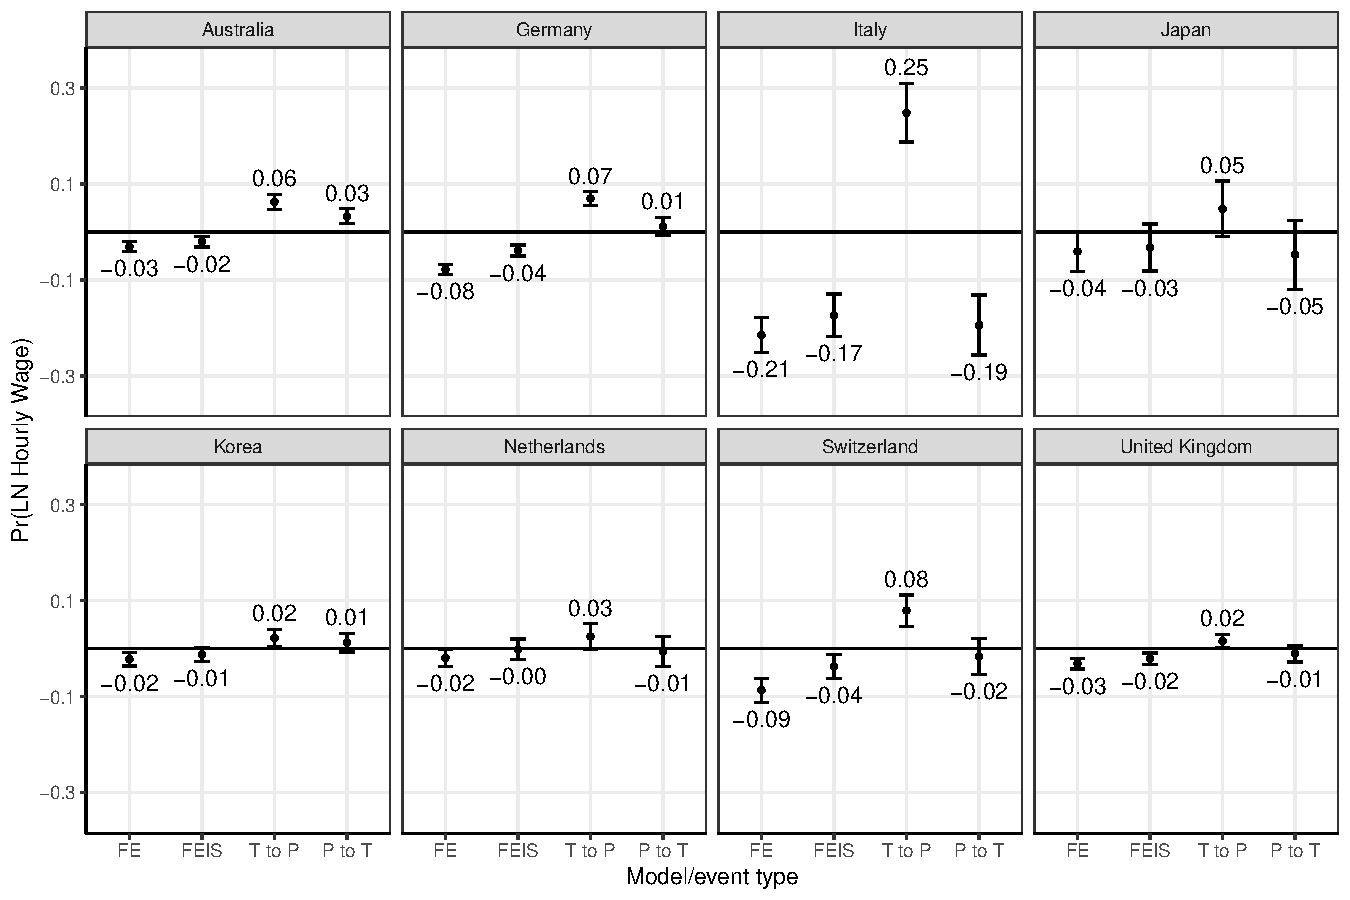
\includegraphics{../graphs/graph_multiple_events_contyp_paper.pdf}}
    \label{graph_contyp}
\end{sidewaysfigure}

\begin{sidewaysfigure}
    \caption{Effect of event on wages over time}
    \resizebox{\textwidth}{!}{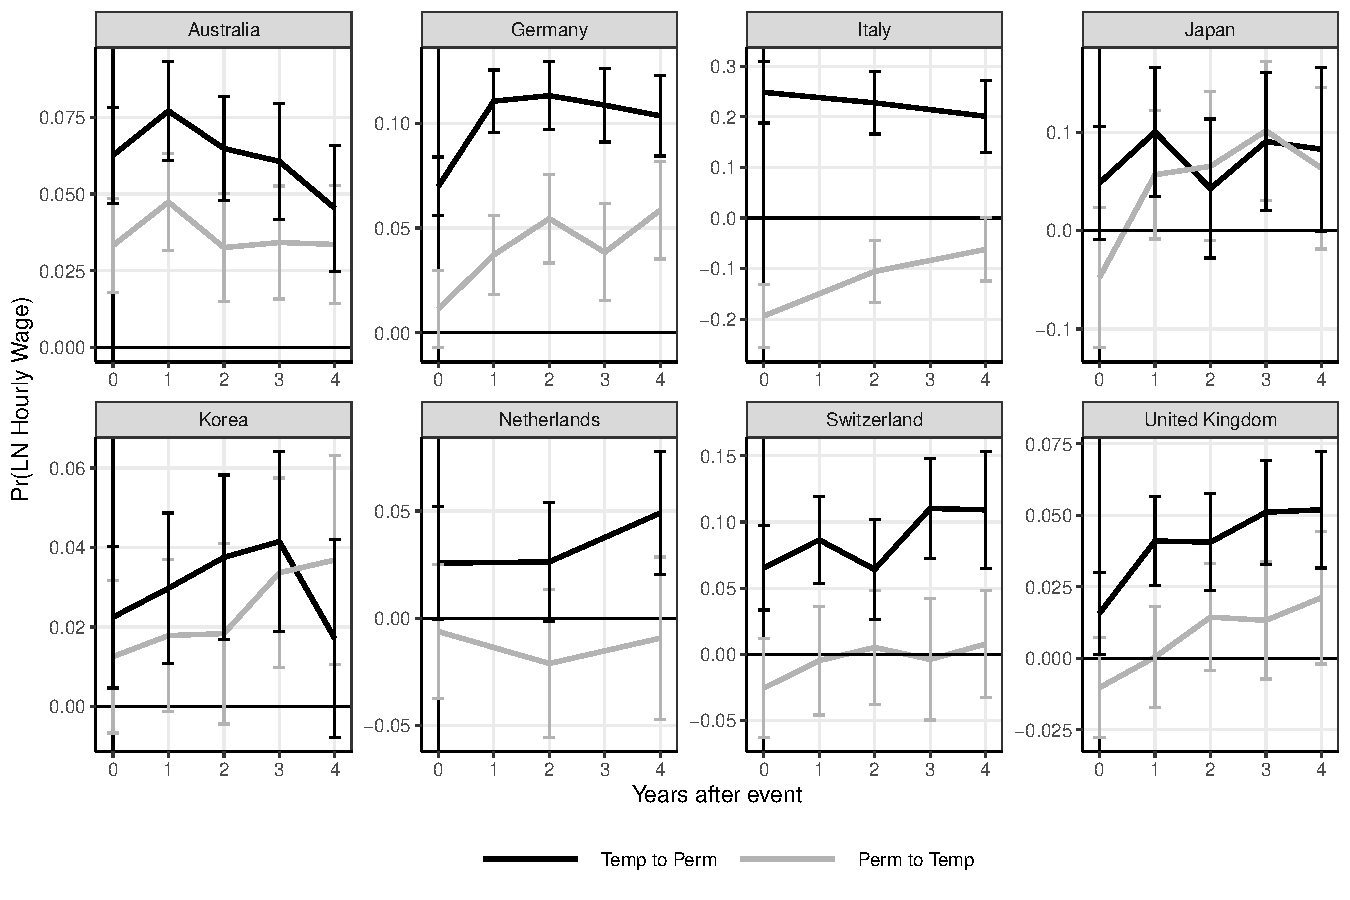
\includegraphics{../graphs/graph_multiple_events_contyp_post_paper.pdf}}
    \label{graph_contyp_post}
\end{sidewaysfigure}

\begin{sidewaysfigure}
    \caption{Effect of event on wages at point in time}
    \resizebox{\textwidth}{!}{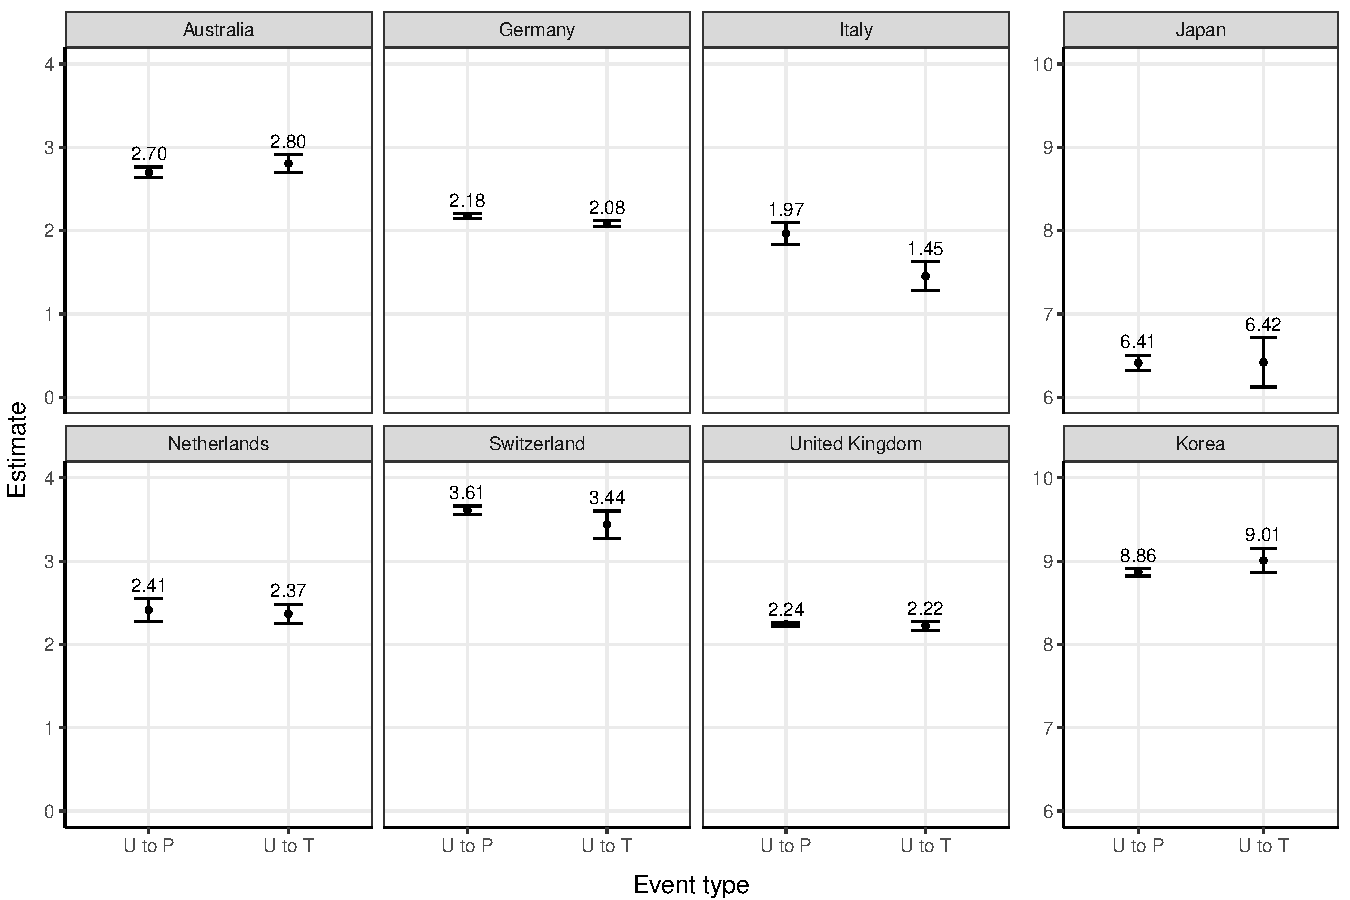
\includegraphics{../graphs/graph_multiple_events_unmp_better_paper.pdf}}
    \label{graph_unmp}
\end{sidewaysfigure}

\begin{sidewaysfigure}
    \caption{Graphical effect of event on wages over time}
    \resizebox{\textwidth}{!}{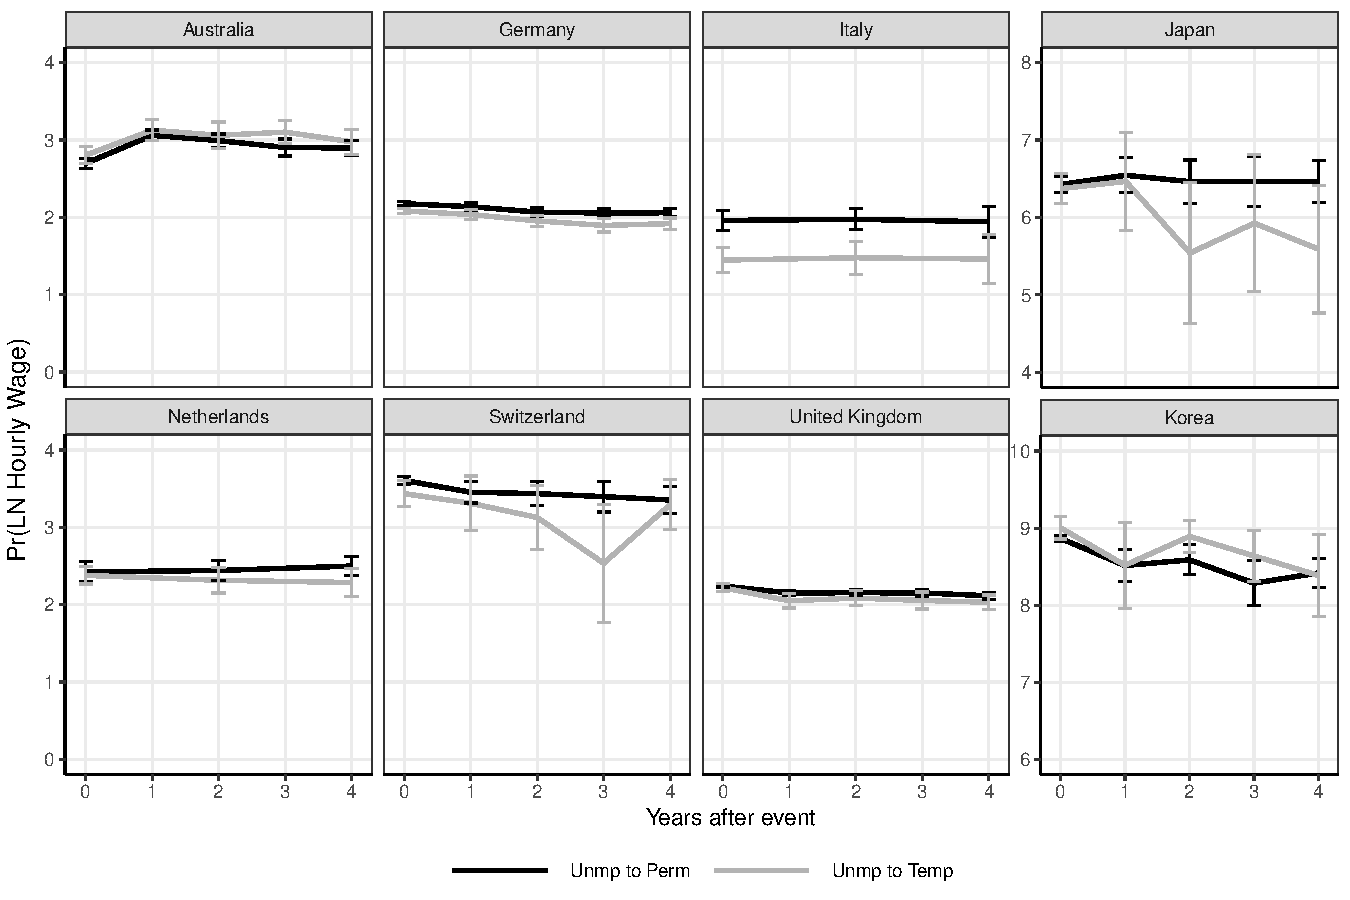
\includegraphics{../graphs/graph_multiple_events_unmp_post_better_paper.pdf}}
    \label{graph_unmp_post}
\end{sidewaysfigure}


%%%%%%%%%%%%%%%%%%%%%%%%%%%%%%%%%%%%%%%%%%
%%%%%%%%%%%%%%%%%%%%%%%%%%%%%%%%%%%%%%%%%%
%%%%%%%%%%%%%%%%%%%%%%%%%%%%%%%%%%%%%%%%%%
%%%%%%%%%%%%%%%%%%%%%%%%%%%%%%%%%%%%%%%%%%

%%%%%%%%%%%%%%%%%%%%%%%%%%
%APPENDIX
%%%%%%%%%%%%%%%%%%%%%%%%%%

\clearpage
\appendix
\setcounter{table}{0}
\setcounter{figure}{0}
\renewcommand*\thetable{\Alph{section}.\arabic{table}}
\renewcommand*\thefigure{\Alph{section}.\arabic{figure}}
\renewcommand{\theHfigure}{\Alph{section}.\arabic{table}}
\renewcommand{\theHtable}{\Alph{section}.\arabic{figure}}

\section{Appendix: Results sensitivity}\label{sec:sensitivity}

\begin{sidewaysfigure}[!h]
    \caption{Australia: All temporary (incl. casual) vs. FTC only (as in the paper)}
    \resizebox{\textwidth}{!}{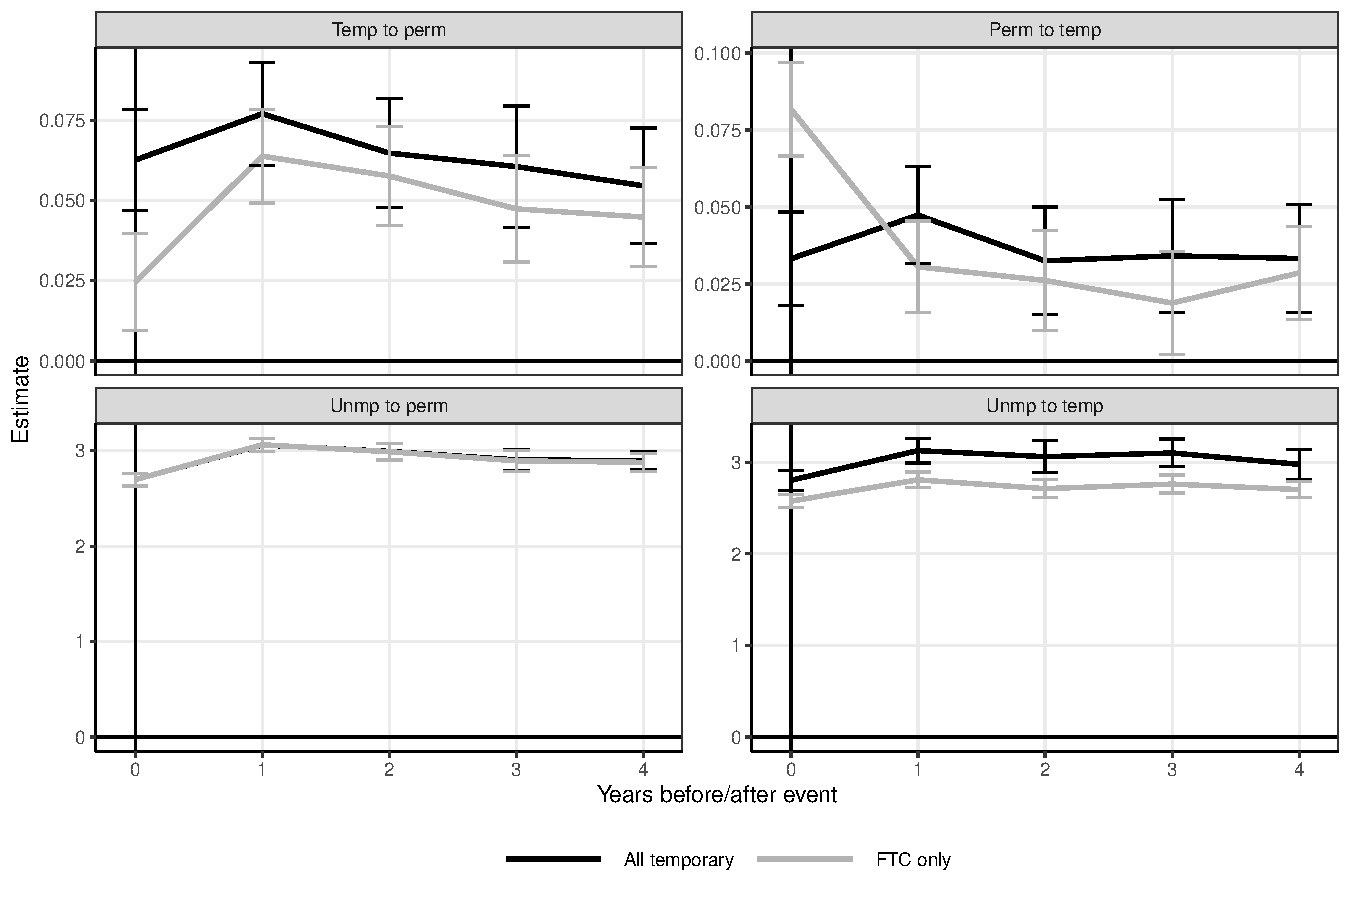
\includegraphics{../graphs/graph_sensitivity_AU_paper.pdf}}
    \label{graph_sensitivity_AU}
\end{sidewaysfigure}

\begin{sidewaysfigure}
    \caption{United Kingdom: All temporary (as in the paper) vs. FTC only}
    \resizebox{\textwidth}{!}{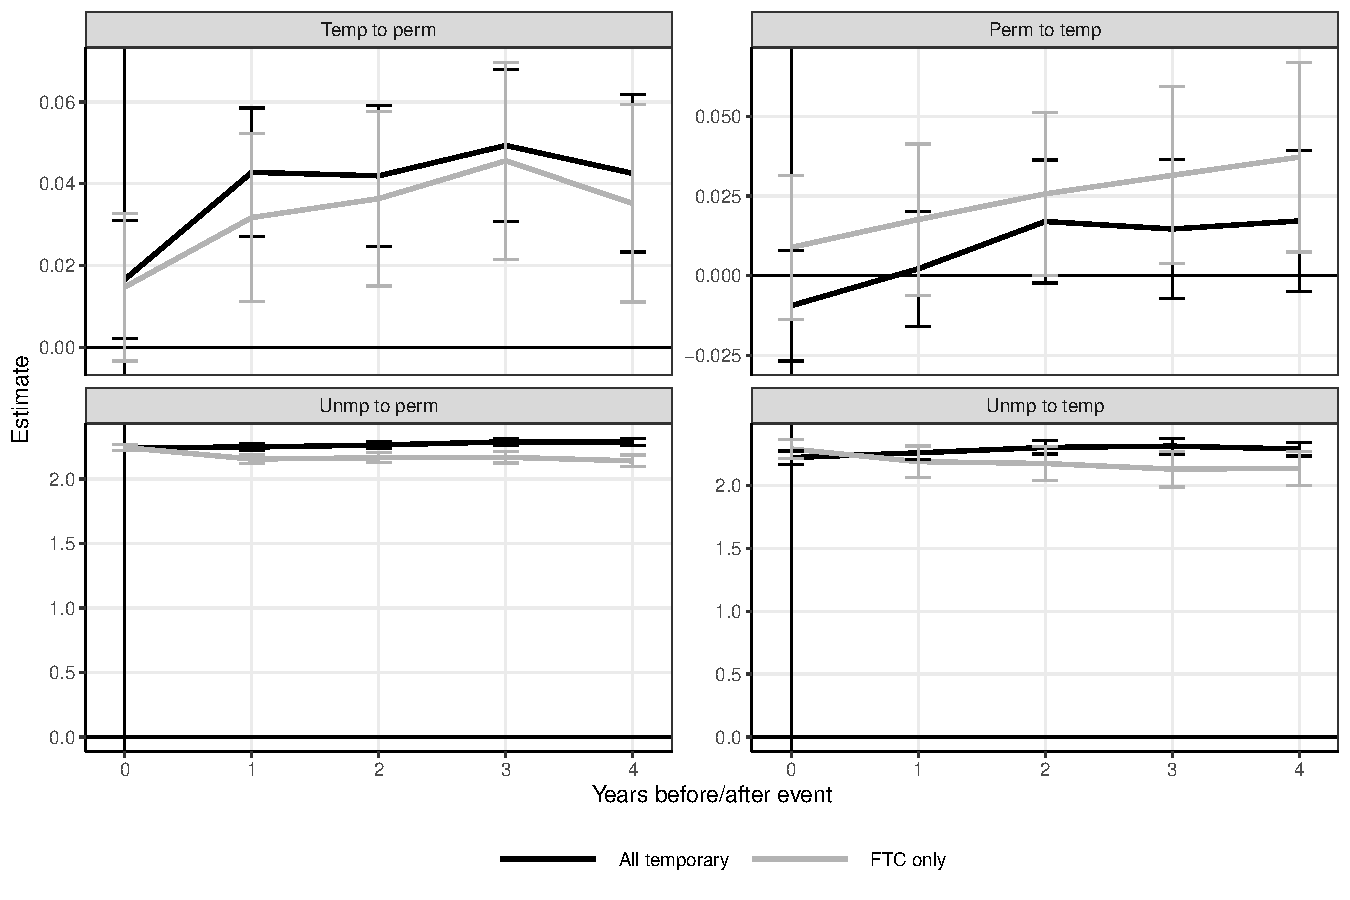
\includegraphics{../graphs/graph_sensitivity_UK_paper.pdf}}
    \label{graph_sensitivity_UK}
\end{sidewaysfigure}

\begin{sidewaysfigure}
    \caption{Netherlands: LSP (as in the paper) vs. LISS}
    \resizebox{\textwidth}{!}{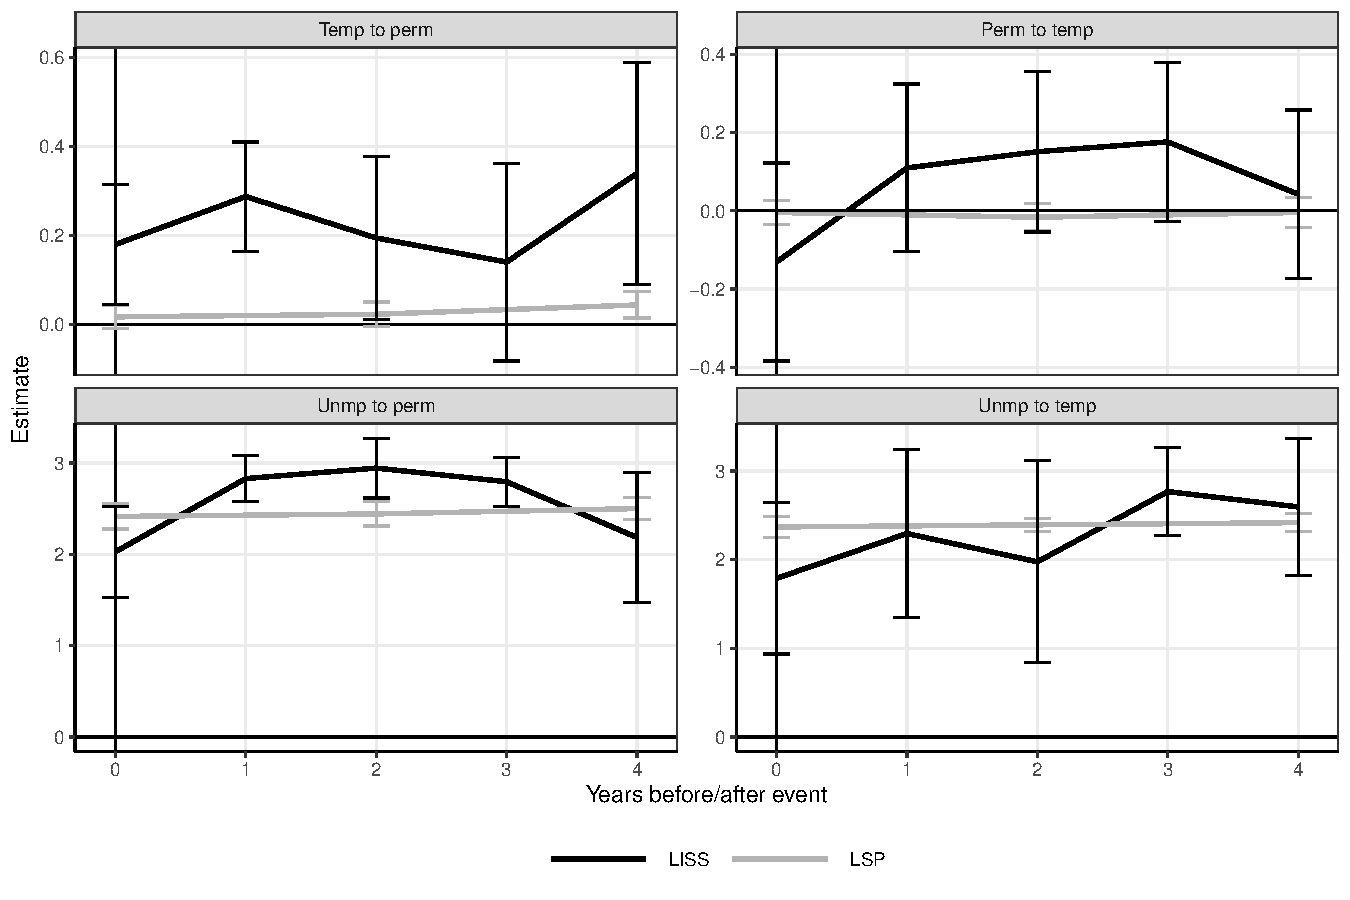
\includegraphics{../graphs/graph_sensitivity_NE_paper.pdf}}
    \label{graph_sensitivity_NE}
\end{sidewaysfigure}

\begin{sidewaysfigure}
    \caption{Methods: FE + IF (as in the paper) vs. FEIS + IF}
    \resizebox{\textwidth}{!}{\includegraphics{../graphs/graph_compare_model_feis_paper.pdf}}
    \label{graph_compare_model_feis}
\end{sidewaysfigure}

%%%%%%%%%%%%%%%%%%%%%%%%%%%%%%%%%%%%%%%%%%
%%%%%%%%%%%%%%%%%%%%%%%%%%%%%%%%%%%%%%%%%%
%%%%%%%%%%%%%%%%%%%%%%%%%%%%%%%%%%%%%%%%%%
%%%%%%%%%%%%%%%%%%%%%%%%%%%%%%%%%%%%%%%%%%
\clearpage
\setcounter{table}{0}
\setcounter{figure}{0}
\renewcommand*\thetable{\Alph{section}.\arabic{table}}
\renewcommand*\thefigure{\Alph{section}.\arabic{figure}}
\renewcommand{\theHfigure}{\Alph{section}.\arabic{table}}
\renewcommand{\theHtable}{\Alph{section}.\arabic{figure}}

\section{Appendix: Results heterogeneity}\label{sec:heterogeneity}

\begin{sidewaysfigure}[!h]
    \caption{Figures \ref{graph_contyp_post} and \ref{graph_unmp_post}, by age category}
    \resizebox{\textwidth}{!}{\includegraphics{../graphs/graph_post_event_age_cat.pdf}}
    \label{graph_post_event_age_cat}
\end{sidewaysfigure}

\begin{sidewaysfigure}[!h]
    \caption{Figures \ref{graph_contyp_post} and \ref{graph_unmp_post}, by education category}
    \resizebox{\textwidth}{!}{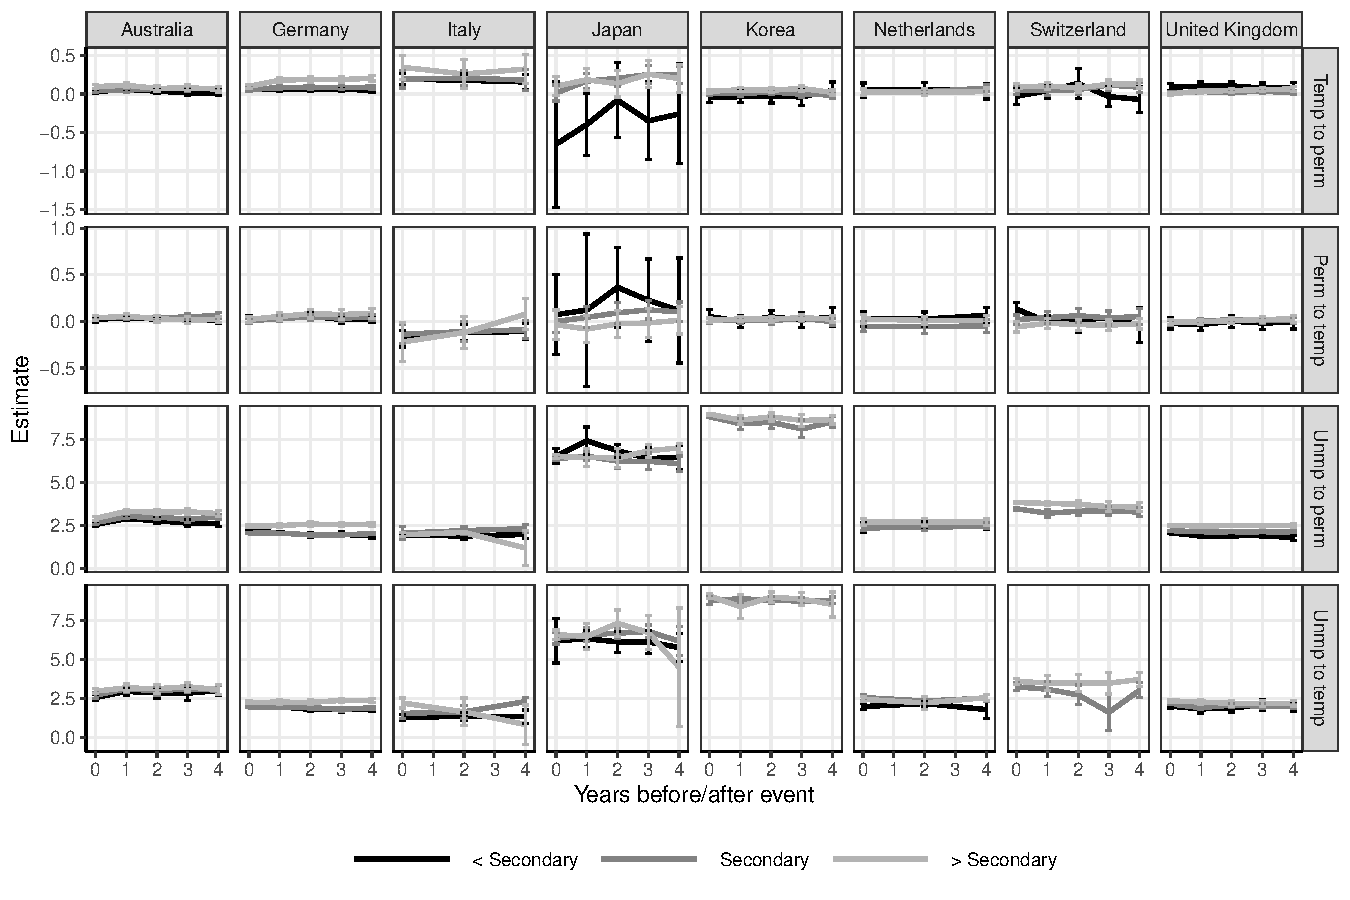
\includegraphics{../graphs/graph_post_event_edu_cat.pdf}}
    \label{graph_post_event_edu_cat}
\end{sidewaysfigure}

\begin{sidewaysfigure}[!h]
    \caption{Figures \ref{graph_contyp_post} and \ref{graph_unmp_post}, by gender}
    \resizebox{\textwidth}{!}{\includegraphics{../graphs/graph_post_event_gender.pdf}}
    \label{graph_post_event_gender}
\end{sidewaysfigure}

%%%%%%%%%%%%%%%%%%%%%%%%%%%%%%%%%%%%%%%%%%
%%%%%%%%%%%%%%%%%%%%%%%%%%%%%%%%%%%%%%%%%%
%%%%%%%%%%%%%%%%%%%%%%%%%%%%%%%%%%%%%%%%%%
%%%%%%%%%%%%%%%%%%%%%%%%%%%%%%%%%%%%%%%%%%
\clearpage
\section{Appendix: Multiple events}\label{sec:multiple}
\setcounter{figure}{0}    
\setcounter{table}{0}    
\renewcommand*\thetable{\Alph{section}.\arabic{table}}
\renewcommand*\thefigure{\Alph{section}.\arabic{figure}}
\renewcommand{\theHfigure}{\Alph{section}.\arabic{table}}
\renewcommand{\theHtable}{\Alph{section}.\arabic{figure}}

As shown in figure \ref{graph_compare_transformed}, let us imagine employment status for one individual in 6 periods of time looks like this (wages): T (50) $\rightarrow$ P (90) $\rightarrow$T (110) $\rightarrow$ P (130) $\rightarrow$ T (140) $\rightarrow$ T (150).  In this case, we may observe four distinct events T $\rightarrow$ P ($\times 2$), and P $\rightarrow$ T ($\times 2$).  In order to model each of the four distinct events, we must transform the data from person, year data into person, event, year data.

The steps are as follows.  First, for each individual, filter one row per individual, transition at the year which the transition occurs ($t_0$).  The result is four rows, one for each event.  Second, create two variables, one to identify each individual, transition ($transeq$) and a second variable for time ($eventtime$), which is 0.  Third, we create a new data frame by selecting only four variables: $pid$, $year$, $transseq$ and $eventtime$.  For each individual, transition ($transseq$), we append rows for $eventtime$ four years before and six years after the transition.  Finally, we merge the new data frame with the original data frame and create a new identifier for each individual, transition sequence ($pidseq$).   

The result is a new data frame with 24 rows: six observations per transition.  The transformed data do not alter the findings obtained by applying FE and FEIS models to untransformed data, as shown in table \ref{table_compare_transformed}.  

\begin{table}[!h]
    \caption{Simulation: Single individual with multiple events}
    \centering
    \resizebox{\textwidth}{!}{
\begin{tabular}{l c c c c c c c}
\toprule
 & \multicolumn{2}{c}{FE} & \multicolumn{2}{c}{FEIS} & \multicolumn{3}{c}{FE + IF} \\
\cmidrule(lr){2-3} \cmidrule(lr){4-5} \cmidrule(lr){6-8}
 & Original & Transformed & Original & Transformed & First & First & Multiple \\
\midrule
Temp                     & $2.50$ & $2.50^{***}$ & $-12.39$ & $-12.39^{***}$ &         &         &           \\
                         & $()$   & $(0.00)$     & $()$     & $(0.00)$       &         &         &           \\
Event: T $\rightarrow$ P &        &              &          &                & $40.00$ &         & $30.00$   \\
                         &        &              &          &                & $$      &         & $(13.05)$ \\
Event: P $\rightarrow$ T &        &              &          &                &         & $20.00$ & $15.00$   \\
                         &        &              &          &                &         & $()$    & $(6.53)$  \\
\midrule
Num. obs.                & $6$    & $24$         & $6$      & $24$           & $6$     & $6$     & $24$      \\
\bottomrule
\multicolumn{8}{l}{\scriptsize{$^{***}p<0.001$; $^{**}p<0.01$; $^{*}p<0.05$. Note: In FE + IF, pre and post event coefficients are not shown.}}
\end{tabular}
}
    \label{table_compare_transformed}
\end{table}

\begin{sidewaysfigure}[!h]
    \caption{Simulation: Single individual with multiple events}
    \resizebox{\textwidth}{!}{\includegraphics{../support_files/simulation/graphs/graph_compare_transformed_data_paper.pdf}}
    \label{graph_compare_transformed}
\end{sidewaysfigure}

\begin{sidewaysfigure}[!h]
    \caption{Compare single vs. multiple events}
    \resizebox{\textwidth}{!}{\includegraphics{../graphs/graph_sensitivity_single_multiple_events_paper.pdf}}
    \label{graph_sensitivity_single_multiple_events}
\end{sidewaysfigure}

\begin{sidewaysfigure}[!h]
    \caption{How many individuals experience multiple events?}
    \resizebox{\textwidth}{!}{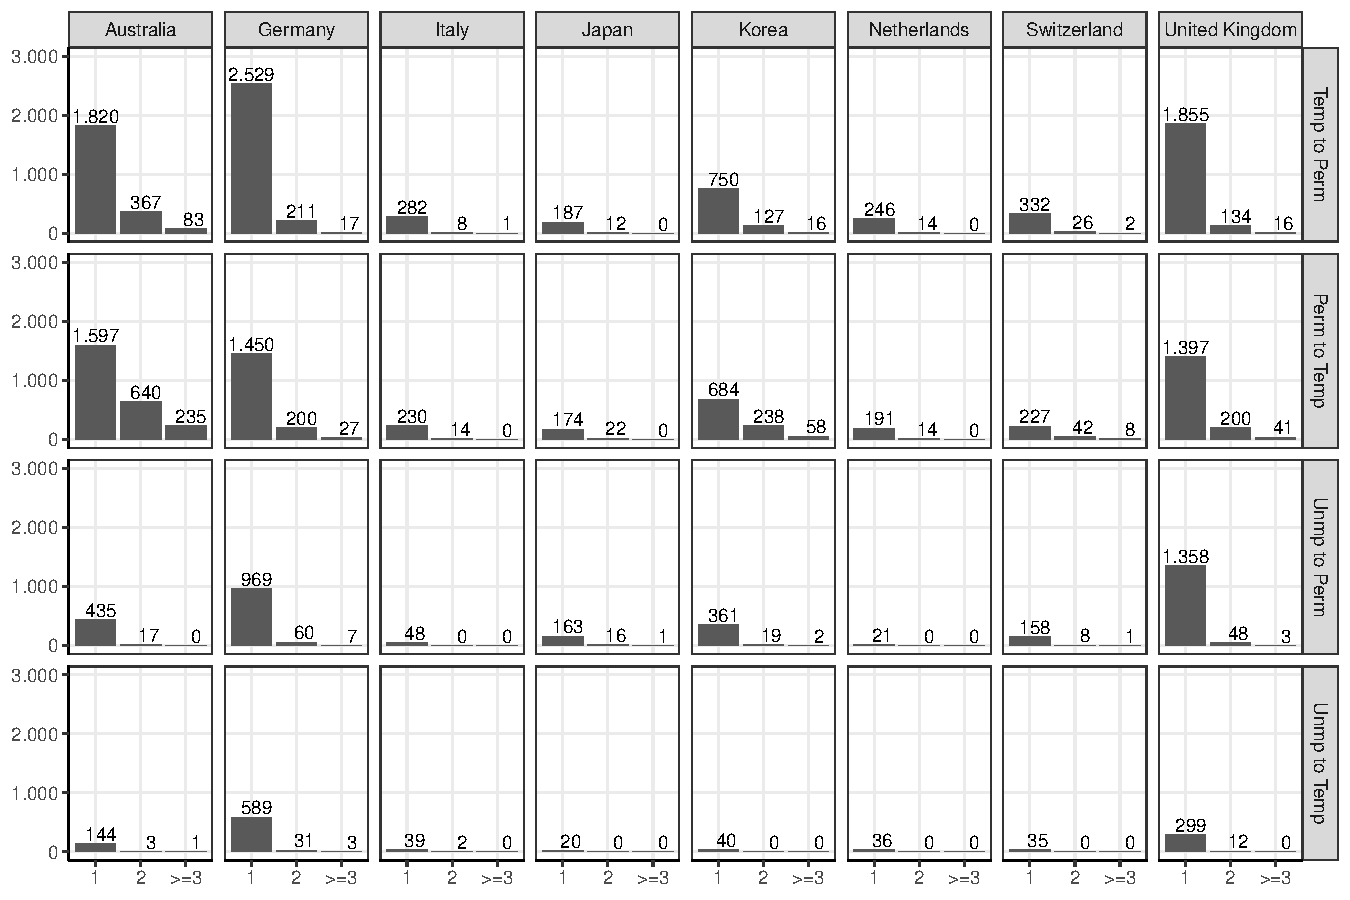
\includegraphics{../graphs/graph_country_events_multiple_presentation_num_paper.pdf}}
    \label{graph_country_events_multiple_presentation_num_paper}
\end{sidewaysfigure}

%%%%%%%%%%%%%%%%%%%%%%%%%%%%%%%%%%%%%%%%%%
%%%%%%%%%%%%%%%%%%%%%%%%%%%%%%%%%%%%%%%%%%
%%%%%%%%%%%%%%%%%%%%%%%%%%%%%%%%%%%%%%%%%%
%%%%%%%%%%%%%%%%%%%%%%%%%%%%%%%%%%%%%%%%%%
\clearpage
\section{Appendix: Sample selection}\label{sec:sample_selection}
\setcounter{figure}{0}    
\setcounter{table}{0}    
\renewcommand*\thetable{\Alph{section}.\arabic{table}}
\renewcommand*\thefigure{\Alph{section}.\arabic{figure}}
\renewcommand{\theHfigure}{\Alph{section}.\arabic{table}}
\renewcommand{\theHtable}{\Alph{section}.\arabic{figure}}

In this appendix, we provide more detail about the sample selection criteria.  Table \ref{table_sample_filter_steps} in the paper details the sample selection criteria, which reduces the sample size by over 50\% in a given country.  Table \ref{table_sample_filter_steps_country} splits table \ref{table_sample_filter_steps} for country.  Table \ref{table_sample_unmp_steps_contyp} specifies why the number of transitions from unemployment to temporary or permanent employment are so small.  The answer is that only about half of individuals who experience unemployment, exit unemployment, and only about a quarter of those who exit are observable as employed within 5 years after the transition (i.e. 3 periods of observation).  More generally, despite sample selection criteria, sample A and B provide similar estimates in a given country, year of average income (LN), unemployment rate, and temporary employment rate as the World Bank  or OECD.  Therefore, the sample are representative of the broader population in a given country.

\begin{sidewaystable}[!h]
    \caption{Sample filter steps from table \ref{table_sample_filter_steps}, by country}
    \centering
    \resizebox{\textwidth}{!}{\begin{tabular}{l>{\raggedright\arraybackslash}p{2.5in}llllllllllllllllll}
   \toprule 
 
\multicolumn{14}{l}{{\bf Panel A:} Sample selection criteria} \\ 

&  & 
\multicolumn{2}{l}{Total (all countries)} &
\multicolumn{2}{l}{Australia} &
\multicolumn{2}{l}{Germany} &
\multicolumn{2}{l}{Italy} &
\multicolumn{2}{l}{Japan} &
\multicolumn{2}{l}{Korea} &
\multicolumn{2}{l}{Netherlands} &
\multicolumn{2}{l}{Switzerland} &
\multicolumn{2}{l}{United Kingdom}
\\  
 
 
\multicolumn{1}{l}{Step} & 
\multicolumn{1}{l}{Description} 
& n & $\Delta$
& n & $\Delta$
& n & $\Delta$
& n & $\Delta$
& n & $\Delta$
& n & $\Delta$
& n & $\Delta$
& n & $\Delta$
& n & $\Delta$
\\ 
\cmidrule(lr){1-2}
\cmidrule(lr){3-4}
\cmidrule(lr){5-6}
\cmidrule(lr){7-8}
\cmidrule(lr){9-10}
\cmidrule(lr){11-12}
\cmidrule(lr){13-14}
\cmidrule(lr){15-16}
\cmidrule(lr){17-18}
\cmidrule(lr){19-20}
\\[-1.8ex]  
 
0 & Raw data & 415,771 &  & 31,951 &  & 91,693 &  & 100,847 &  & 10,499 &  & 24,491 &  & 14,458 &  & 34,469 &  & 107,363 &  \\ 
  1 & Panel years between 2000 and 2018 & 367,032 & -12\% & 31,951 & 0\% & 83,722 & -9\% & 68,012 & -33\% & 10,499 & 0\% & 23,515 & -4\% & 14,458 & 0\% & 34,469 & 0\% & 100,406 & -6\% \\ 
  2 & Prime age (25 - 54) & 210,900 & -43\% & 19,431 & -39\% & 52,198 & -38\% & 33,724 & -50\% & 6,315 & -40\% & 16,089 & -32\% & 9,693 & -33\% & 17,205 & -50\% & 56,245 & -44\% \\ 
  3 & Unemployed or employed with contract type, monthly hours (40 -- 320), and wages $>$ 0 & 157,370 & -25\% & 15,881 & -18\% & 38,538 & -26\% & 25,547 & -24\% & 4,787 & -24\% & 10,980 & -32\% & 7,461 & -23\% & 9,251 & -46\% & 44,925 & -20\% \\ 
  4 & Non missing education or gender & 155,535 & -1\% & 15,875 & 0\% & 37,635 & -2\% & 25,547 & 0\% & 4,767 & 0\% & 10,978 & 0\% & 7,449 & 0\% & 9,251 & 0\% & 44,033 & -2\% \\ 
  5 & Hourly wages within the top/bottom 0.005 percentile & 154,743 & -1\% & 15,817 & 0\% & 37,454 & 0\% & 25,336 & -1\% & 4,754 & 0\% & 10,943 & 0\% & 7,404 & -1\% & 9,168 & -1\% & 43,867 & 0\% \\ 
  6 & Data set A: At least 3 observations & 79,148 & -49\% & 10,598 & -33\% & 20,972 & -44\% & 3,678 & -85\% & 3,179 & -33\% & 7,311 & -33\% & 2,418 & -67\% & 5,303 & -42\% & 25,689 & -41\% \\ 
  7 & Data set B: + always employed & 73,189 & -8\% & 10,072 & -5\% & 18,302 & -13\% & 3,449 & -6\% & 3,079 & -3\% & 7,103 & -3\% & 2,320 & -4\% & 5,153 & -3\% & 23,711 & -8\% \\ 
   
\hline \\[-1.8ex]  
 
\multicolumn{14}{l}{{\bf Panel B:} Data sets by event type (if treated, must be employed after treatment)} \\ 

& 
& \# & \%
& \# & \%
& \# & \%
& \# & \%
& \# & \%
& \# & \%
& \# & \%
& \# & \%
& \# & \%
\\ 
\cmidrule(lr){1-2}
\cmidrule(lr){3-4}
\cmidrule(lr){5-6}
\cmidrule(lr){7-8}
\cmidrule(lr){9-10}
\cmidrule(lr){11-12}
\cmidrule(lr){13-14}
\cmidrule(lr){15-16}
\cmidrule(lr){17-18}
\cmidrule(lr){19-20}
\\[-1.8ex]  
 
A & Unmp $\rightarrow$ perm & 3,670 & 5\% & 452 & 4\% & 1,036 & 5\% & 48 & 1\% & 155 & 5\% & 382 & 5\% & 21 & 1\% & 167 & 3\% & 1,409 & 5\% \\ 
  A & Unmp $\rightarrow$ temp & 1,268 & 2\% & 148 & 1\% & 623 & 3\% & 41 & 1\% & 34 & 1\% & 40 & 1\% & 36 & 1\% & 35 & 1\% & 311 & 1\% \\ 
  B & Temp $\rightarrow$ perm & 9,063 & 12\% & 2,270 & 23\% & 2,757 & 15\% & 291 & 8\% & 227 & 7\% & 893 & 13\% & 260 & 11\% & 360 & 7\% & 2,005 & 8\% \\ 
  B & Perm $\rightarrow$ temp & 6,800 & 9\% & 1,992 & 20\% & 1,559 & 9\% & 237 & 7\% & 232 & 8\% & 822 & 12\% & 198 & 9\% & 250 & 5\% & 1,510 & 6\% \\ 
   \bottomrule \\[-1.8ex] \multicolumn{20}{p{12in}}{Note: n - is unique observations.  $\Delta$ - is difference in n from previous step.  \# - is unique n who experienced at least 1 event.  \% - is percent who experienced an event.} 
\end{tabular}
}
    \label{table_sample_filter_steps_country}
\end{sidewaystable}

\begin{sidewaystable}[!h]
    \caption{Why are the number of unemployment exits so small?}
    \centering
    \resizebox{\textwidth}{!}{\begin{tabular}{l>{\raggedright\arraybackslash}p{2in}llllllllllllllllll}
   \\[-1.8ex]\hline\hline \\ 
 [-1.8ex]
\multicolumn{20}{l}{{\bf Panel A:} Sample selection criteria} \\ 

&  & 
\multicolumn{2}{l}{Total (all countries)} &
\multicolumn{2}{l}{Australia} &
\multicolumn{2}{l}{Germany} &
\multicolumn{2}{l}{Italy} &
\multicolumn{2}{l}{Japan} &
\multicolumn{2}{l}{Korea} &
\multicolumn{2}{l}{Netherlands} &
\multicolumn{2}{l}{Switzerland} &
\multicolumn{2}{l}{United Kingdom}
\\  
 
 
\multicolumn{1}{l}{Step} & 
\multicolumn{1}{l}{Description} 
& n & $\Delta$
& n & $\Delta$
& n & $\Delta$
& n & $\Delta$
& n & $\Delta$
& n & $\Delta$
& n & $\Delta$
& n & $\Delta$
& n & $\Delta$
\\ 
\cmidrule(lr){1-2}
\cmidrule(lr){3-4}
\cmidrule(lr){5-6}
\cmidrule(lr){7-8}
\cmidrule(lr){9-10}
\cmidrule(lr){11-12}
\cmidrule(lr){13-14}
\cmidrule(lr){15-16}
\cmidrule(lr){17-18}
\cmidrule(lr){19-20}
\\[-1.8ex]  
 
1 & Total unemployment events (From data set A) & 14,450 &  & 1,917 &  & 5,562 &  & 335 &  & 364 &  & 980 &  & 184 &  & 531 &  & 4,577 &  \\ 
  2 & Must exit unemployment & 6,463 & -55\% & 1,060 & -45\% & 2,079 & -63\% & 145 & -57\% & 212 & -42\% & 478 & -51\% & 90 & -51\% & 256 & -52\% & 2,143 & -53\% \\ 
  3 & Employed at least 1 period after exit (within 5 years) & 4,847 & -25\% & 592 & -44\% & 1,608 & -23\% & 86 & -41\% & 184 & -13\% & 419 & -12\% & 56 & -38\% & 199 & -22\% & 1,703 & -21\% \\ 
   
\hline \\[-1.8ex]  
 
\multicolumn{20}{l}{{\bf Panel B:} Frequency, by event type} \\ 

& 
&  \# & \%
&  \# & \%
&  \# & \%
&  \# & \%
&  \# & \%
&  \# & \%
&  \# & \%
&  \# & \%
&  \# & \%
\\ 
\cmidrule(lr){1-2}
\cmidrule(lr){3-4}
\cmidrule(lr){5-6}
\cmidrule(lr){7-8}
\cmidrule(lr){9-10}
\cmidrule(lr){11-12}
\cmidrule(lr){13-14}
\cmidrule(lr){15-16}
\cmidrule(lr){17-18}
\cmidrule(lr){19-20}
\\[-1.8ex]  
 
 & Unmp $\rightarrow$ temp & 1,268 & 26\% & 148 & 25\% & 623 & 39\% & 41 & 48\% & 34 & 18\% & 40 & 10\% & 36 & 64\% & 35 & 18\% & 311 & 18\% \\ 
   & Unmp $\rightarrow$ perm & 3,670 & 76\% & 452 & 76\% & 1,036 & 64\% & 48 & 56\% & 155 & 84\% & 382 & 91\% & 21 & 38\% & 167 & 84\% & 1,409 & 83\% \\ 
   & U $\rightarrow$ P \& U $\rightarrow$ T & 91 &  & 8 &  & 51 &  & 3 &  & 5 &  & 3 &  & 1 &  & 3 &  & 17 &  \\ 
   \hline \\[-1.8ex] \multicolumn{20}{p{12in}}{Notes: n - is unique observations.  
               $\Delta$ - is difference in n from previous step.  
               \# - is number of transitions.  
               \% - is percent of total transitions from step 3. 
               \% is more than 100\% because some individuals experience both a transition from Unmp to Perm and Unmp to Temp.} 
\end{tabular}
}
    \label{table_sample_unmp_steps_contyp}
\end{sidewaystable}



\begin{sidewaysfigure}[!h]
    \caption{Compare annual average income (LN) from sample to OECD}
    \resizebox{\textwidth}{!}{\includegraphics{../graphs/graph_descriptives_income_better_paper.pdf}}
    \label{graph_descriptives_income_better_paper.pdf}
\end{sidewaysfigure}

\begin{sidewaysfigure}[!h]
    \caption{Compare unemployment rate from sample to World Bank}
    \resizebox{\textwidth}{!}{\includegraphics{../graphs/graph_descriptives_unmp_paper.pdf}}
    \label{graph_descriptives_unmp_paper}
\end{sidewaysfigure}

\begin{sidewaysfigure}[!h]
    \caption{Compare temporary employment rate from sample to OECD}
    \resizebox{\textwidth}{!}{\includegraphics{../graphs/graph_descriptives_temp_paper.pdf}}
    \label{graph_descriptives_temp_paper}
\end{sidewaysfigure}

\end{document}



%%%%%%%%%%%%%%%%%%%%%%%%%%%%%%%%
% BIBLIOGRAPHY
%%%%%%%%%%%%%%%%%%%%%%%%%%%%%%%%

\clearpage
\singlespacing
\bibliographystyle{apalike2}
\bibliography{references}

\clearpage
\appendix

%%%%%%%%%%%%%%%%%%%%%%%%%%
%APPENDIX
%%%%%%%%%%%%%%%%%%%%%%%%%%

\section{Appendix: Data sets}\label{appendix:data}
\setcounter{figure}{0}    
\setcounter{table}{0}    
\renewcommand*\thetable{\Alph{section}.\arabic{table}}
\renewcommand*\thefigure{\Alph{section}.\arabic{figure}}
\renewcommand{\theHfigure}{\Alph{section}.\arabic{table}}
\renewcommand{\theHtable}{\Alph{section}.\arabic{figure}}

We use 9 different data sets from 8 countries:

\begin{enumerate}
    \item Australia: Australia panel data are from the Household, Income and Labour Dynamics in Australia \citep{hilda_household_2022}.  HILDA is a longitudinal survey that has been following members of a nationally representative sample of Australian households on an annual basis since 2001 \citep{watson_wooden_2012}.  In 2001, the survey contained data on nearly 14,000 individuals in nearly 7,700 households.  As of 2018, the HILDA Survey included data from approximately 17,500 individuals in around 9,500 households across Australia.  The HILDA Survey includes information about employment and earnings for sample participants that are 15 years or older.  

    \item Germany: German panel data are from the Socio-Economic Panel \citep{soep_2020}.  SOEP is a longitudinal study of private households in Germany.  The survey is conducted annually.  Sample A, often called the `West German Sample', began in 1984 and included West Germany, both Germans and foreigners.  Sample B, `Foreigners in the Federal Republic of Germany', was also created in 1984 in order to over sample foreigners that were under represented in Sample A.  Sample C was begun in 1990 to include German residents of the German Democratic Republic (GDR).  Since then, numerous refresher samples were added in order to supplement panel attrition \citep{soep_jan_2019}.  In 2000, the SOEP included data from around approximately 22.000 individuals in 12,000 households. By 2018, the SOEP contained information from about 32,000 individuals in about 19,000 households across Germany.

    \item Italy: Since the 1960s, the Bank of Italy has conducted the Survey on Household Income and Wealth  \citep{shiw_historical_2019} biannually. Its primary objective is to amass comprehensive data regarding the individual and households family composition and employment status.   Since 1989, the sample included households previously interviewed going back to 1977.  However, the survey only includes data on contract type since 2000.  In 2000, the survey included data on approximately 14,000 individuals in 8,000 households.  By 2016, the survey includes data on nearly 70,000 individuals in nearly 40,000 households.  As we noted in the main document, we do not include panel data after 2016.  In 2022, The Bank of Italy released the 2022 survey wave for SHIW, which contains data up to 2020, but skips the 2020 biannual survey wave, which would have contained data up to 2018.  As a result, if we were to use the 2022 wave, there would be a four-year gap between 2020 and 2016, not a two-year gap between 2020 and 2018 or 2018 and 2016 as should be the case if the 2020 panel wave was released.

    \item Japan: Japanese panel data are harmonized from the Keio Household Panel Survey and the Japan Household Panel Survey \citep{jhpskhps_keio_2019}.  Both are annual surveys.  The KHPS has been implemented annually since 2004 on 4,000 households and 7,000 individuals nationwide.  In 2009, the JHPS began as a new survey targeting 4,000 male and female individuals in parallel with the KHPS.  The two data sets are harmonized prior to release by the agency responsible for making the data available to researchers.  As of 2018, the survey includes data on nearly 10,000 individuals.  

    \item Korea: Korean panel data are from the Korea Labor and Income Panel Study \citep{klips_korean_2020}.  It is an annual survey of urban households members who are at least 15 years of age or older that began in 1998.  In 1999, the first year it included data on approximately 13,000 individuals in 5,000 households.  By 2018, the survey includes data on nearly 25,000 individuals.

    \item Netherlands: We use two panel data sets for the Netherlands.  
    \begin{enumerate}
        \item Arbeidsaanbodpanel or Labour Supply Panel \citep{lsp_arbeidsaanbodpanel_2016} - We use the LSP as our main source of panel data.  Begun in 1985, it is a biannual long-term survey of the Dutch working population (aged 16 - 66) and their employment situation.  Unfortunately, the LSP ended in 2014.
        \item Longitudinal Internet Studies for the Social Sciences \citep{liss_longitudinal_2020} - We use the LISS as a sensitivity for the LSP.  The LISS is not a replacement for the LSP.  Begun in 2007, it is an annual survey of 5,000 households, comprising approximately 7.500 individuals, 16 years of age or older.  Unique among all other panel data, panel participants complete online questionnaires every month.  As a result, non-internet users are absent.  Without denying the advantages and value of the LISS, the survey does suffer from high levels of panel attrition, as shown in table \ref{table_sample_filter_steps_country_NE}.
    \end{enumerate}

    \item Switzerland: Swiss panel data are from the Swiss Household Panel \citep{shp_swiss_2020}.  The SHP is conducted by the Swiss Foundation for Research in Social Sciences (FORS).  Available since 1999, it is an annual survey that interviews all household members over the age of 14 from a random sample of private households in Switzerland, stratified across the seven major statistical regions of Switzerland.  The SHP combines three samples: the SHP I (5,074 households and 7,799 individuals interviewed first in 1999), the SHP II (2,538 households and 3,654 individuals interviewed first in 2004) and the SHP III (3,989 households and 6,090 individuals interviewed first in 2013).  In total, there are nearly 16,000 individuals in nearly 10,000 households.  

    \item United Kingdom: Panel data from the United Kingdom are harmonized from the British Household Panel Study (BHPS) and the United Kingdom Household Longitudinal Study \citep{bhpsukhls_university_2022}.  Both are annual surveys.  Begun in 1991, the BHPS followed the same representative sample of individuals.  In 2008, as part of wave 18, BHPS participants were asked if they would consider joining the new, larger, more wide-ranging survey called Understanding Society or UKHLS.  Therefore, the UKHLS is considered a supplement and extension of the original BHPS.  BHPS and UKHLS data are harmonized, allowing researchers to analyze data since 1991.

\end{enumerate}

With the exception of panel data from the Netherlands and Italy, most of our data are available in the CNEF.  As noted by Tillmann et al. \citeyearpar[pg. vii]{tillmann2018social}, ``The fact that the panels in CNEF are comparable is not a lucky accident, but rather an important feature of the worldwide social and behavioral sciences research infrastructure. A concerted effort ensures that these panel studies are comparable in terms of the basic setups and the questionnaires.''  

%%%%%%%%%%%%%%%%%%%%%%%%%%%%%%%%%%%%%%%%%%
%%%%%%%%%%%%%%%%%%%%%%%%%%%%%%%%%%%%%%%%%%
%%%%%%%%%%%%%%%%%%%%%%%%%%%%%%%%%%%%%%%%%%
%%%%%%%%%%%%%%%%%%%%%%%%%%%%%%%%%%%%%%%%%%

\clearpage
\setcounter{table}{0}
\setcounter{figure}{0}
\renewcommand*\thetable{\Alph{section}.\arabic{table}}
\renewcommand*\thefigure{\Alph{section}.\arabic{figure}}
\renewcommand{\theHfigure}{\Alph{section}.\arabic{table}}
\renewcommand{\theHtable}{\Alph{section}.\arabic{figure}}

\section{Appendix: Recoding variables}\label{appendix:variables}

One cannot dismiss the methodological challenges associated with comparing data from national panel surveys given large differences in sampling and survey design. Input harmonized is the process of standardizing or normalizing data inputs before they are collected and entered into a system to ensure that data collected from different sources follow a standardized format and coding scheme (i.e. EU-SILC).  By contrast, output harmonized is the process of recoding the data after it has been collected in order to align data to a common set of variables, codes, and classification.  While CNEF/CPF refer to their data as `harmonized,' they may be better characterized as output harmonized and accurately understood as recoding, as we do here.  

In order to compare across variables in different data sets, we recoded five variables: employment status, employment contract, hours, wages and salary from a person's main job, education.  With the exception of top codes and missing cases, four variables require no recoding: age, gender, person ID, year.  

We also include a variable for country-level unemployment rate, which comes from World Bank data, not OECD because OECD does not include Switzerland before 2010, after 2010, both data sources are the same. 

The dependent variable is log of hourly wages.  To create a variable for hourly wage, hours and wages are recoded into monthly values to compare across data sets.  Wages are either monthly or annually, but hours are often weekly, with the exception of Germany where hours are annual.  Hourly wages are created by dividing monthly wages by monthly hours worked.    Once we create a variable for hourly wages, wages are inflation adjusted to the year 2010 using the country-specific, CPI index from the World Bank.  Wages are represented in the national currency and are not adjusted using any equivalence scale.  

Employment status is recoded into a categorical variable with two levels indicating, employed or unemployed and looking for work.  This is shown in figure \ref{graph_descriptives_emp_status}.  Unemployment is variously defined by country.  If not stated, then we assume that `unemployed' is defined as unemployed, but looking for work.  We do not use additional survey items on whether a respondent is looking for work while being unemployed.  

Employed is further specified as an individual with an observable contract type with observable monthly hours between 40 and 320 (i.e. no less than 10 hours per week and no more than 80 hours per week.


Education.  We do not control for education as it is usually time-invarying for adult participants in the labour force.  However, we do split the analysis by education group as a sensitivity test (see Appendix \ref{appendix:sensitivity_heterogeneity}.  Most countries use ISCED, but some countries do not.  For example, Germany uses CASMIN, Australia codes educational attainment in accordance with the Australia Bureau of Statistics (ABS) approach, and the Netherlands and Japan use their own definition.  Education is recoded into a categorical variable with three levels indicating, less than secondary education, secondary education, and more than secondary education.  This is shown in figure \ref{graph_descriptives_education}.

The remaining variable is employment contract.  We measure temporary employment following OECD/Eurostat definitions to indicate if a contract is `permanent' or  `not permanent,' i.e. temporary in some way.  This is shown in figure \ref{graph_descriptives_contyp}.  

The single country exception is Australia, where we define `not permanent' as a fixed term contract (FTC).  This definition excludes casual work, a distinct type of employment relationship that is less comparable to temporary work in other countries because it offers a wage premium in exchange for the loss of other benefits \citep{mooi-reci_casual_2017}.  However, results over time after the first period are qualitatively similar if we include casual employment (as shown in the Appendix \ref{appendix:sensitivity_variable}, figure \ref{graph_sensitivity_AU}).  

If we exclude missing or unknown levels, then three countries, Switzerland (variable: pw36), Germany (variable: plb0037), and Korea (variable: p\_\_0501) use a single variable to ask whether the job duration is limited in some way, yes or no.  In Switzerland, a separate variable is used to specify the limited nature of the contract (variable pw37: apprenticeship, trial period, etc.).  For details on Switzerland, see figure \ref{graph_ch_compare_sample_age} in Appendix \ref{appendix:sensitivity_sample}.

Another five countries split temporary into two categories.  In Australia (variable: gjbmcnt), temporary employment is defined as either a `fixed term contract' or `casual basis'; in Italy (variable: contratt), temporary employment is defined as `fixed term' or `temporary'; in the Netherlands (variable: eb002), temporary employment is defined as either `temporary to permanent' or  `temporary'.  In Japan, employment status (v219) is split into seven categories, of which three are temporary: `contract employee', `subcontracted worker', and `specialized contract employee'.  

In the United Kingdom, before 1999, (variable: jbterm), temporary employment is defined as `seasonal/tmp' or  `contract/fixed time', after 1999 (variable: jbterm1), there is only permanent and not permanent.  Instead, like in Switzerland, a separate variable is used to specify the limited nature of the contract (variable jbterm2:).  Using jbterm2, we can distinguish work that is `Done under contract for a fixed period or a fixed task' from other types of temporary work, `seasonal', `agency', `casual', etc.  However, results are qualitatively similar if we include isolate temporary work that is done under a fixed term contract, form other types of temporary work (as shown in the Appendix \ref{appendix:sensitivity_variable}, figure \ref{graph_sensitivity_UK}).  

Unlike Australia or the United Kingdom, we do not perform a similar sensitivity check for Switzerland because all temporary work is a fixed-term contract that is limited in duration by time.

We do not suggest that temporary or permanent contracts are the same between countries nor do we suggest that all temporary contracts are the same within countries.  For this reason, wages of temporary workers are not directly compared across countries, but within countries and within persons in comparison to permanent work and unemployment.  Instead, the key point is that there is a bigger difference between permanent and temporary contracts than within temporary contracts.  

\begin{sidewaysfigure}[h!]
    \caption{Recode employment status by country}
    \resizebox{\textwidth}{!}{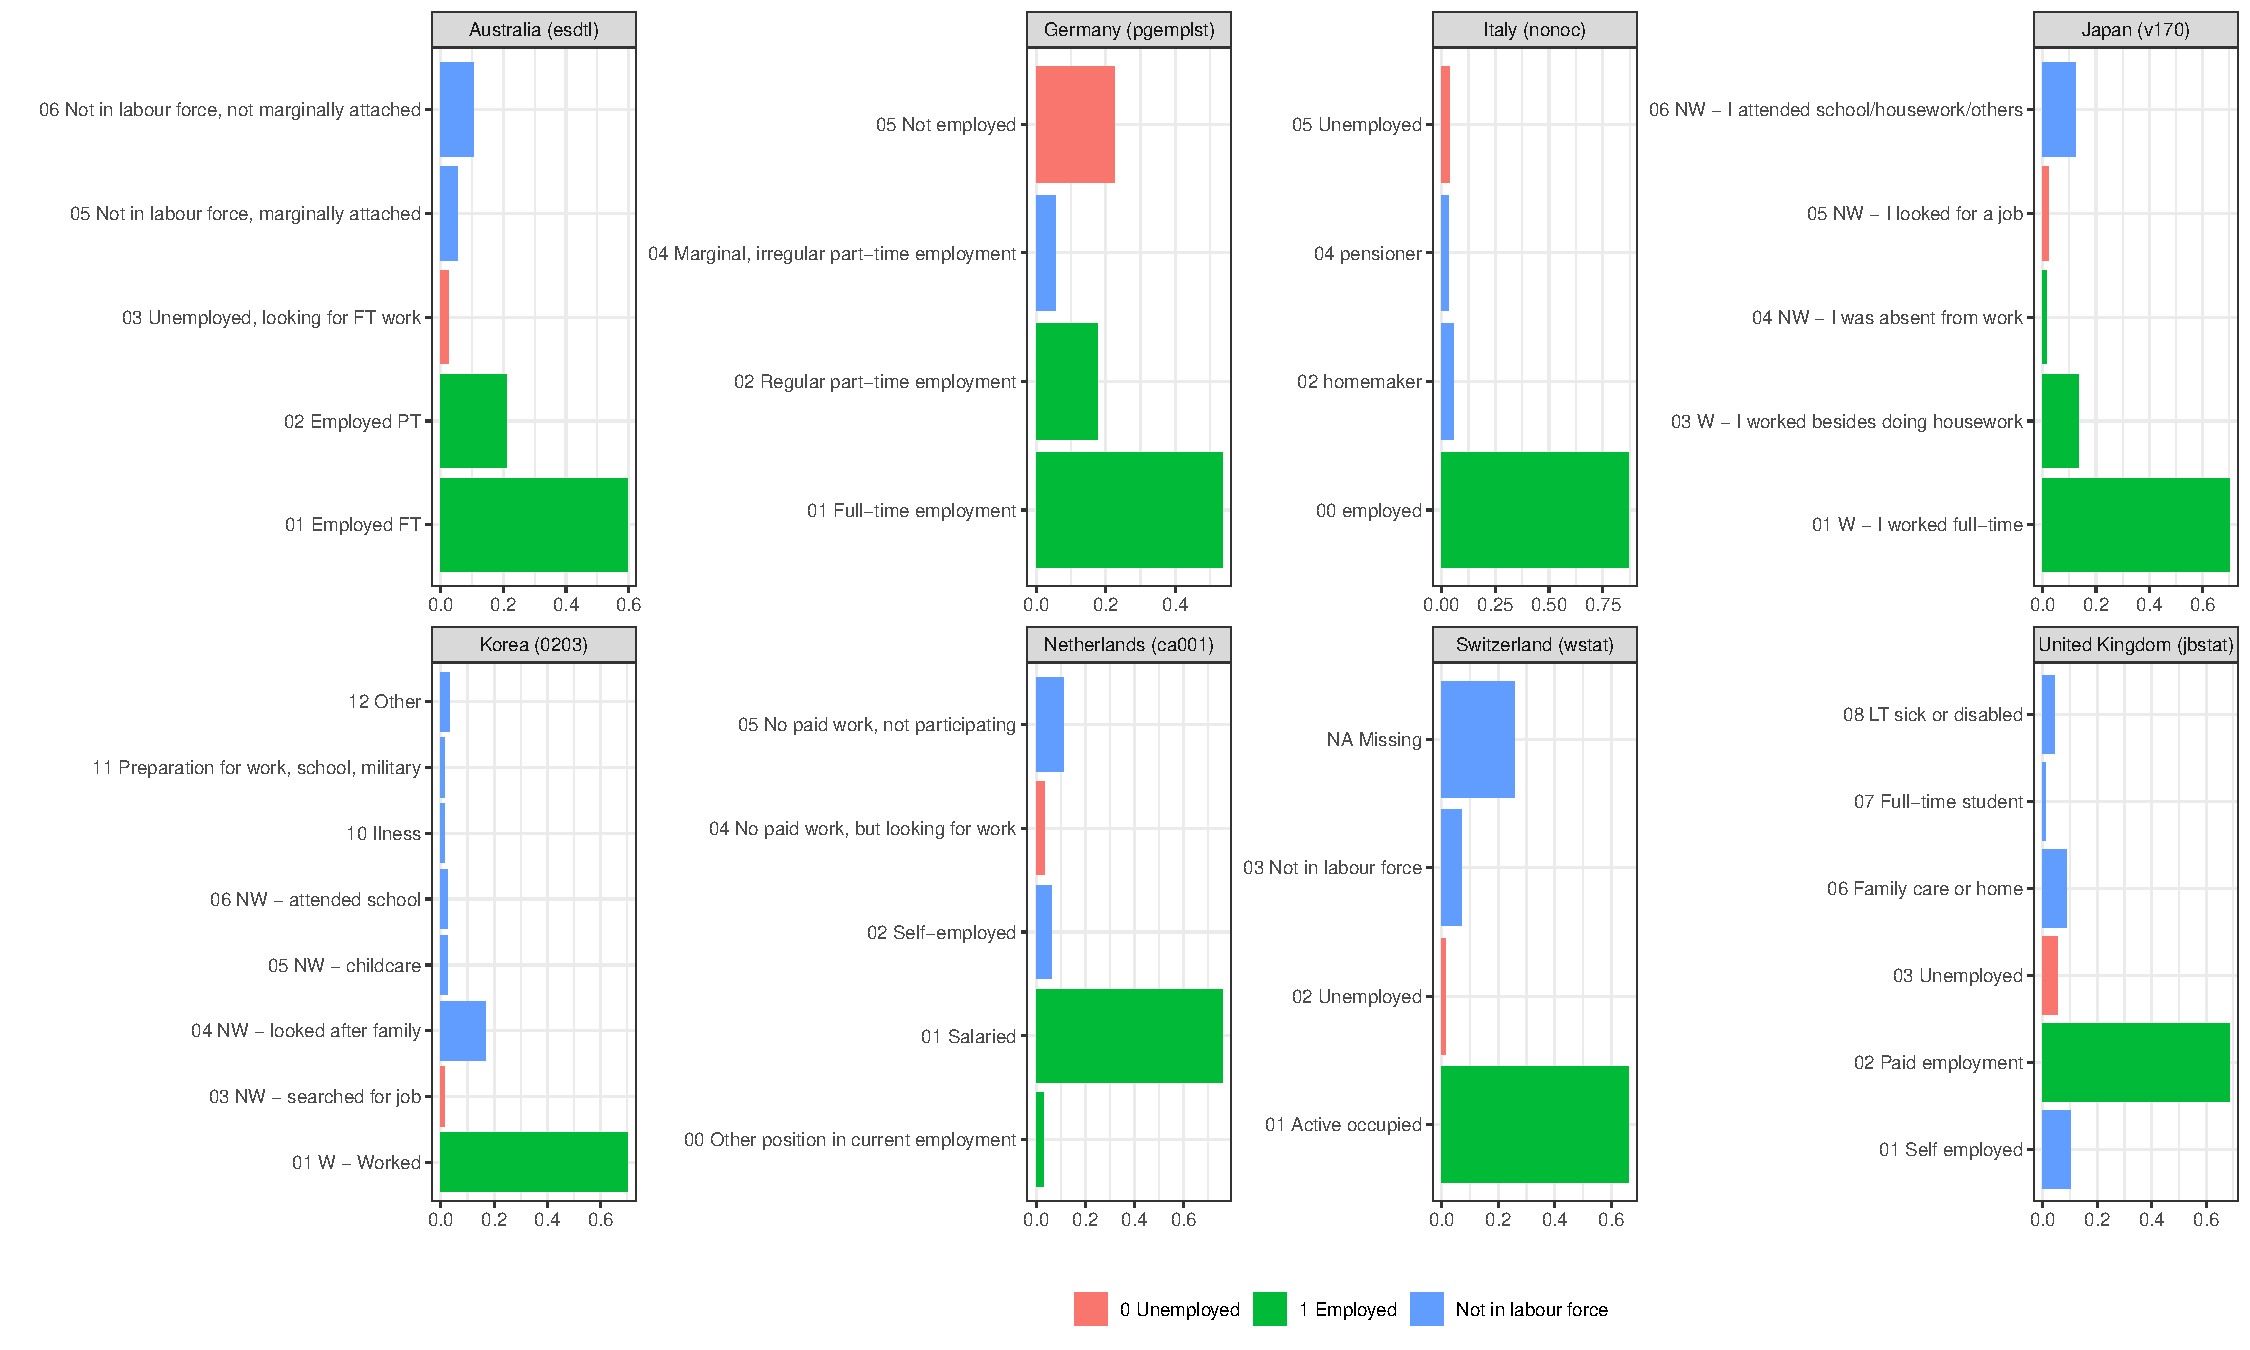
\includegraphics{../../../graphs/descriptives/graph_descriptives_emp_status.pdf}}
    \label{graph_descriptives_emp_status}
\end{sidewaysfigure}

\begin{sidewaysfigure}[h!]
    \caption{Recode contract type by country (conditional on employed with contract)}
    \resizebox{\textwidth}{!}{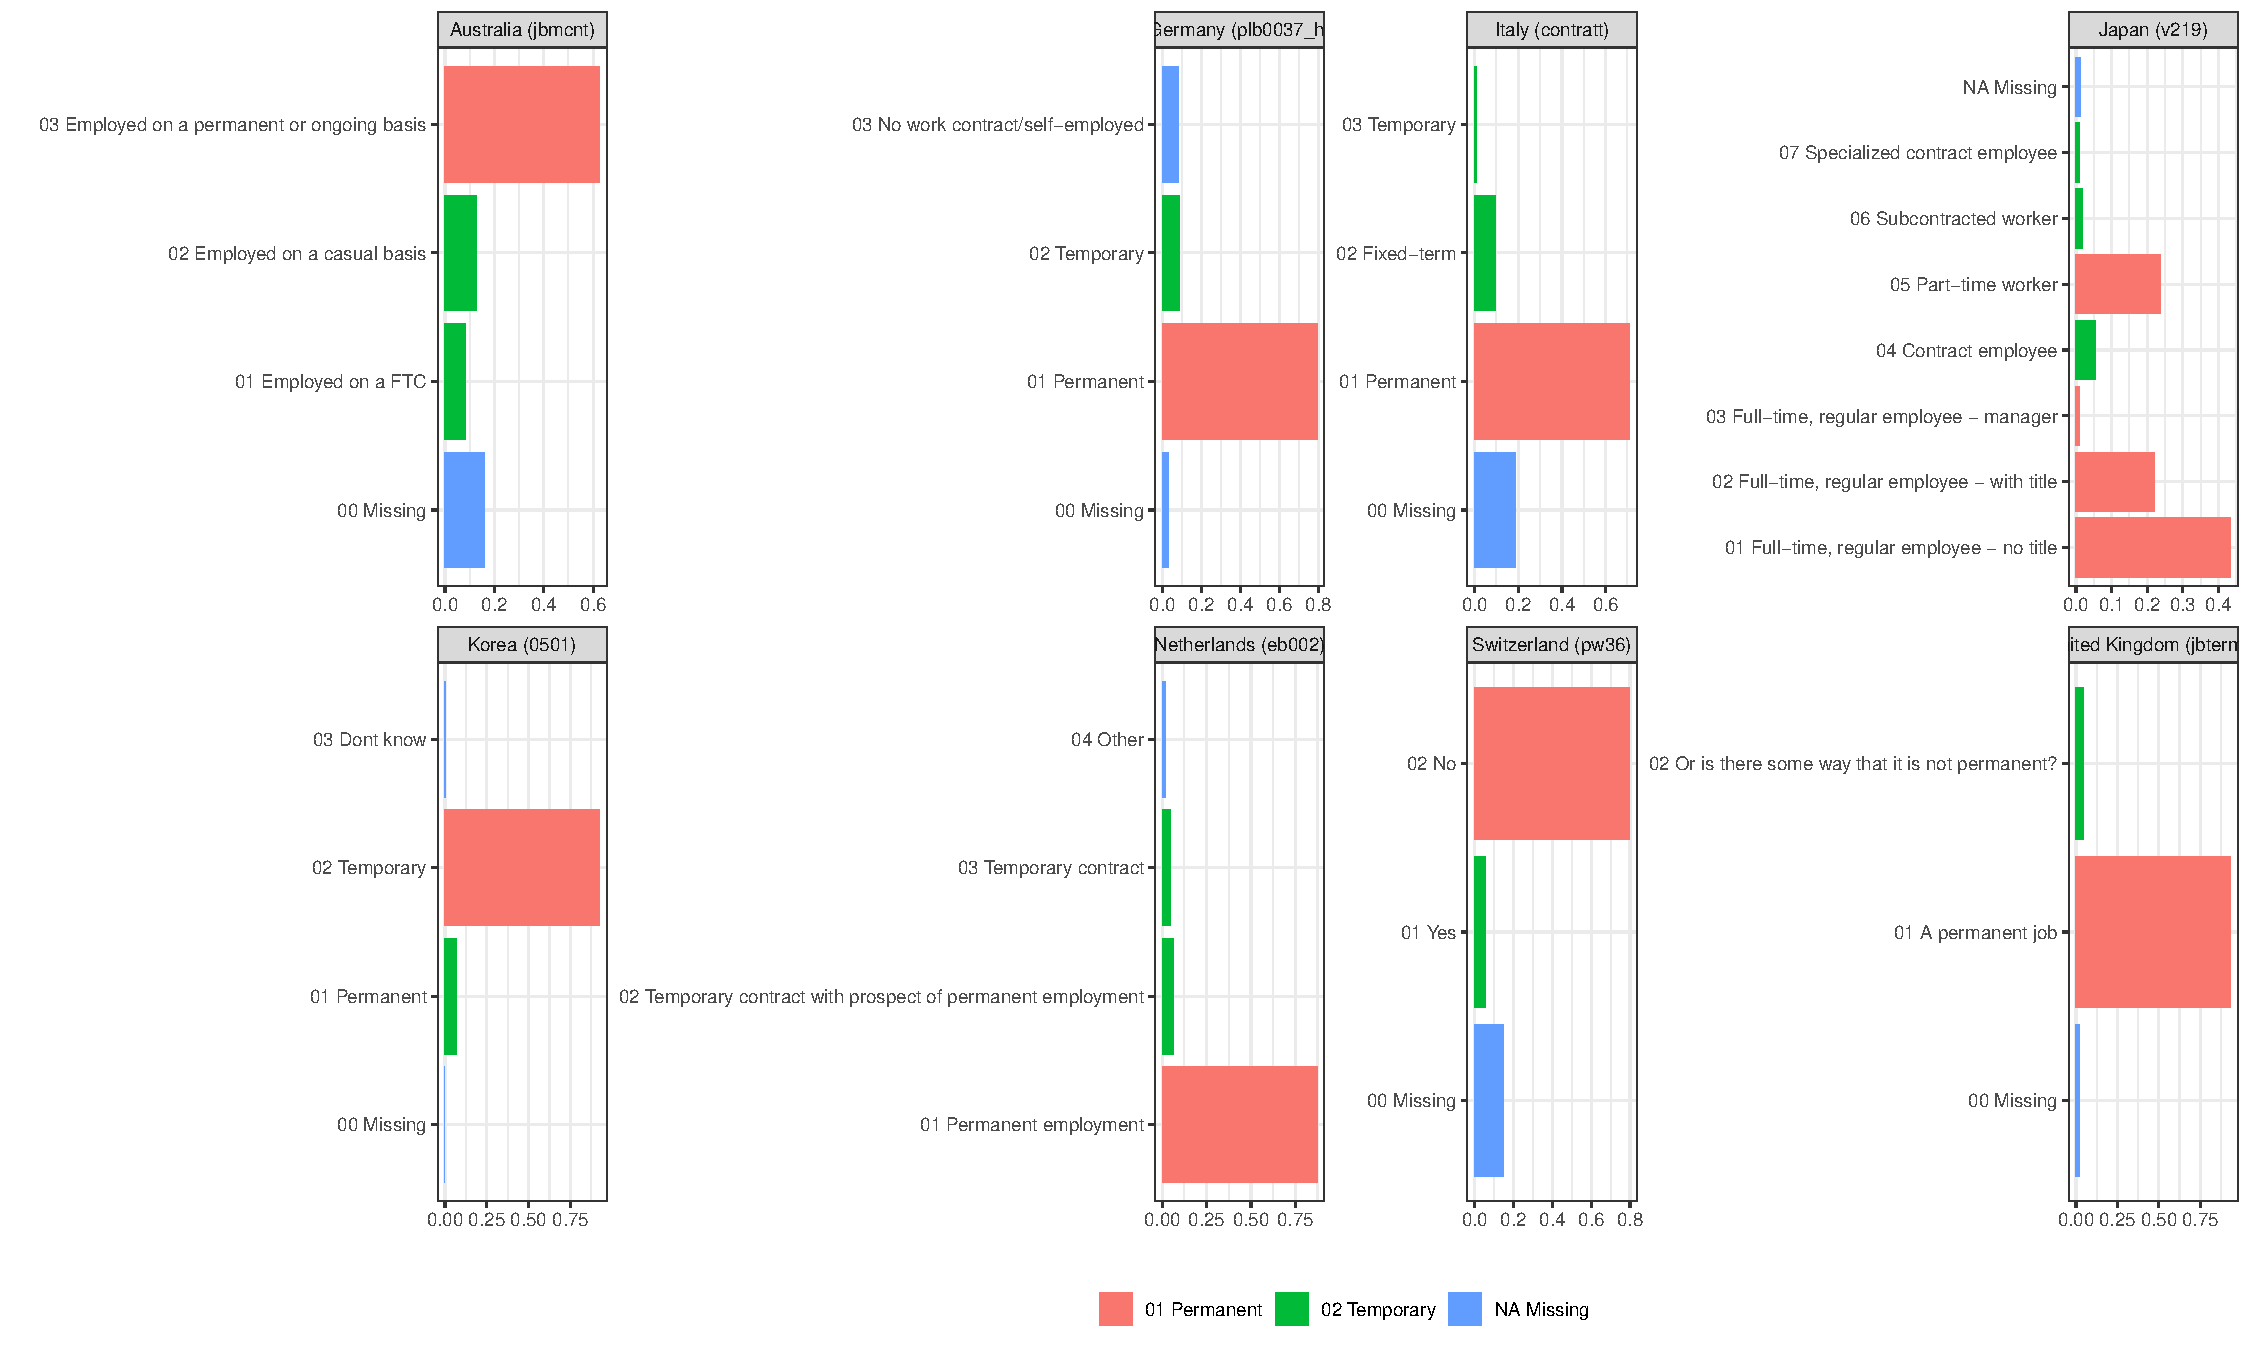
\includegraphics{../../../graphs/descriptives/graph_descriptives_contyp.pdf}}
    \label{graph_descriptives_contyp}
\end{sidewaysfigure}

\begin{sidewaysfigure}[h!]
    \caption{Recode education by country}
    \resizebox{\textwidth}{!}{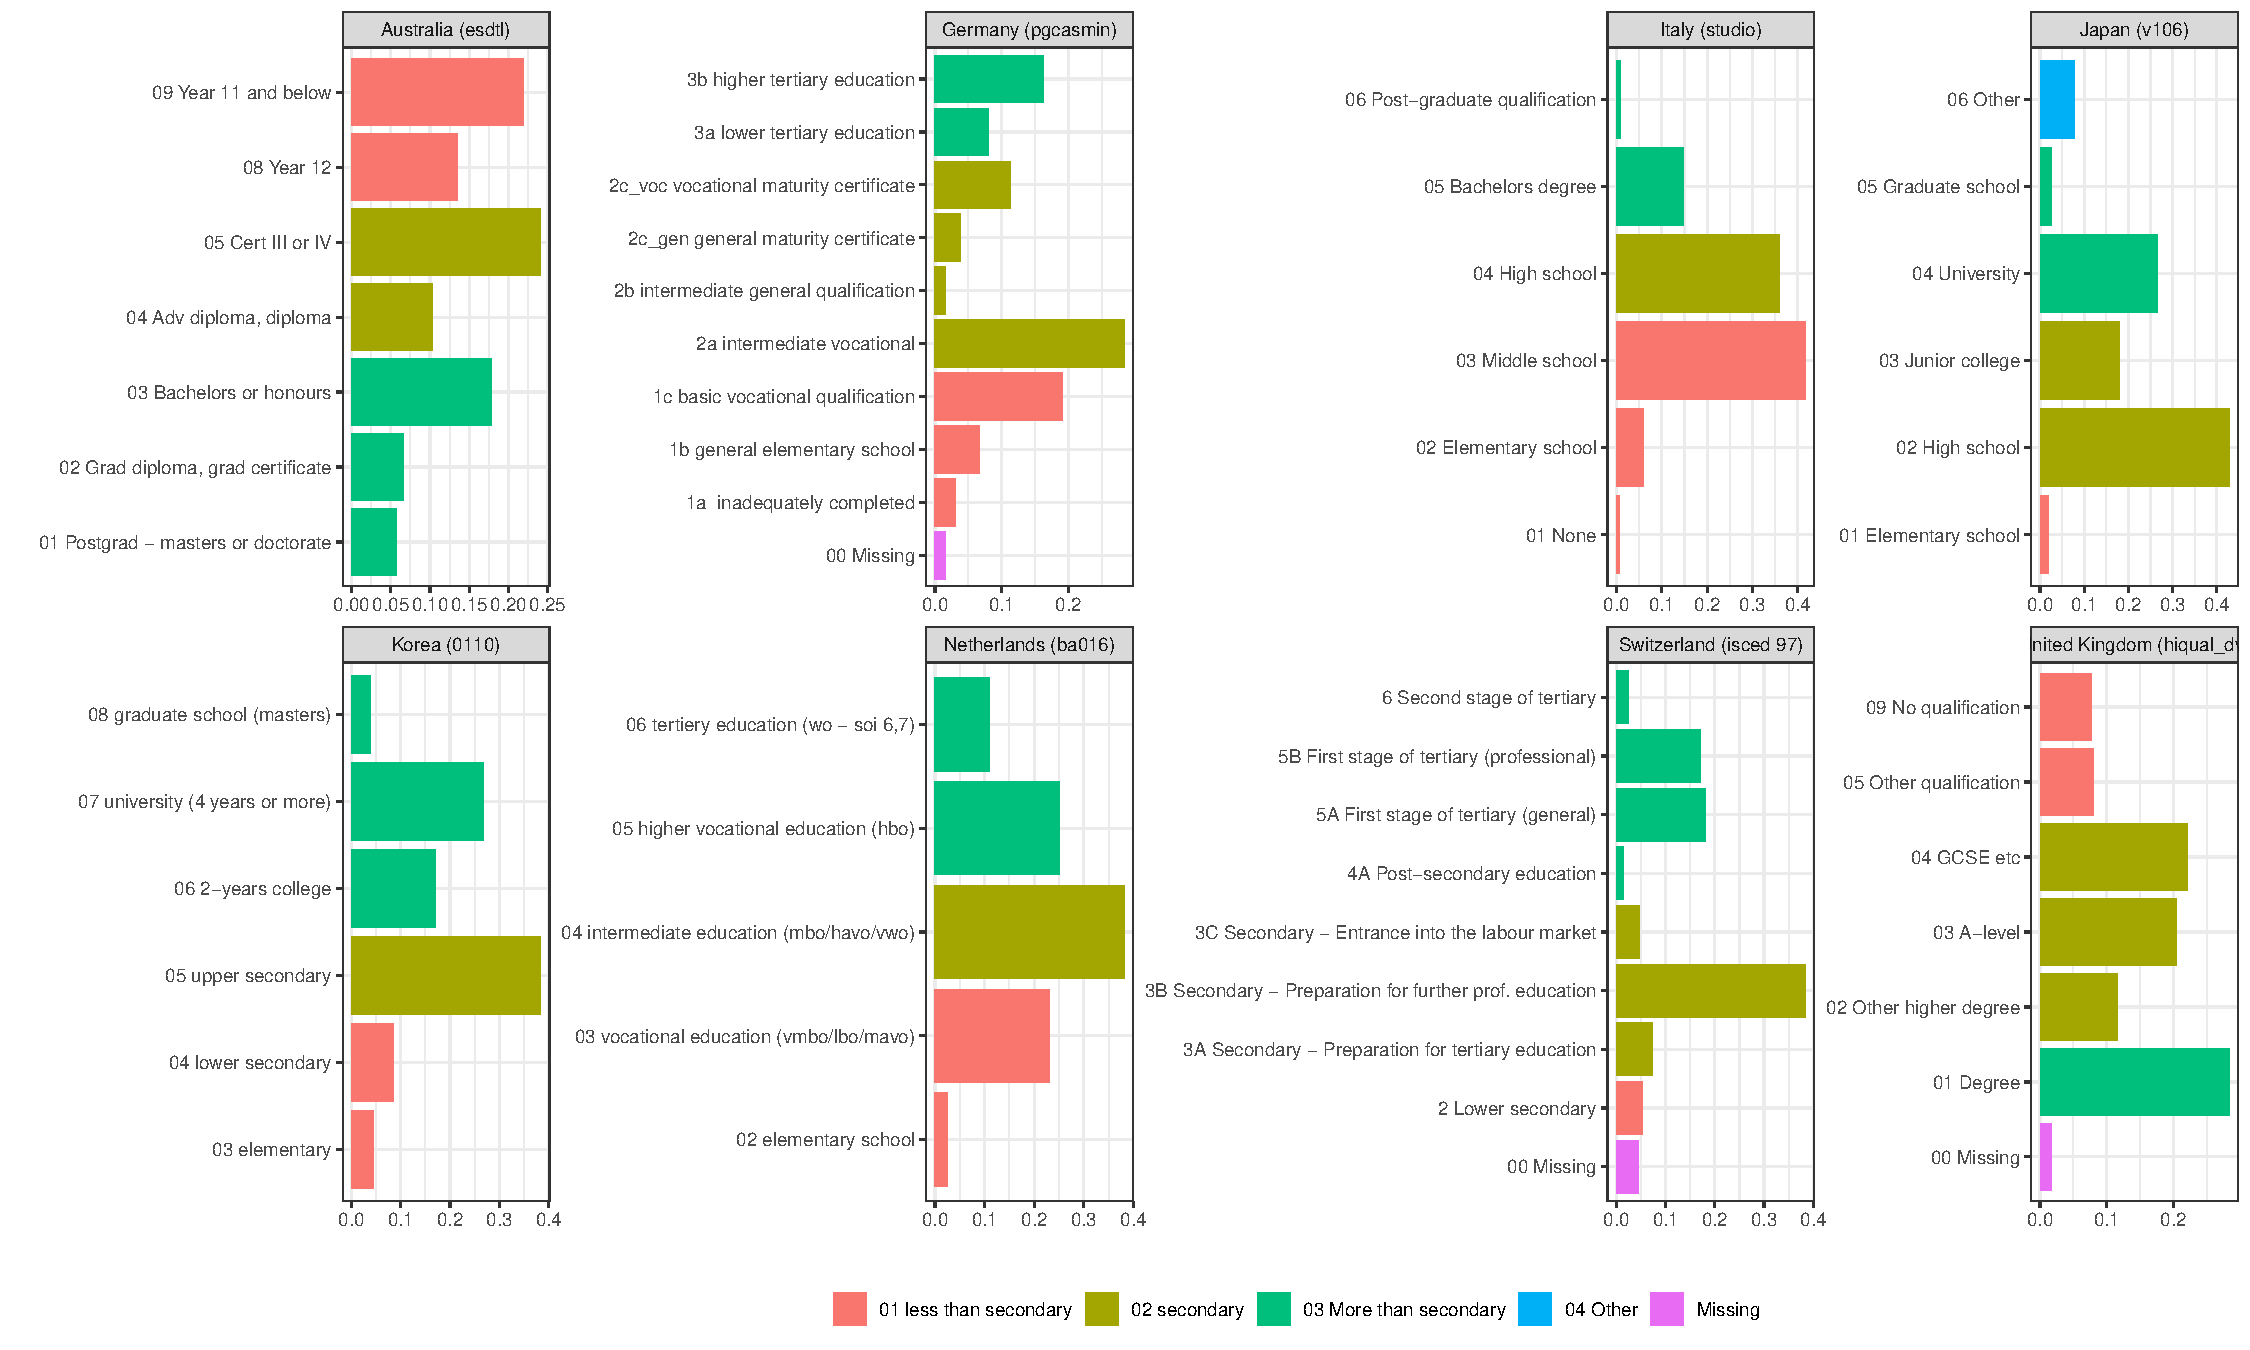
\includegraphics{../../../graphs/descriptives/graph_descriptives_education.pdf}}
    \label{graph_descriptives_education}
\end{sidewaysfigure}


%%%%%%%%%%%%%%%%%%%%%%%%%%%%%%%%%%%%%%%%%%
%%%%%%%%%%%%%%%%%%%%%%%%%%%%%%%%%%%%%%%%%%
%%%%%%%%%%%%%%%%%%%%%%%%%%%%%%%%%%%%%%%%%%
%%%%%%%%%%%%%%%%%%%%%%%%%%%%%%%%%%%%%%%%%%
\clearpage
\section{Appendix: Sample selection}\label{appendix:sample_selection}
\setcounter{figure}{0}    
\setcounter{table}{0}    
\renewcommand*\thetable{\Alph{section}.\arabic{table}}
\renewcommand*\thefigure{\Alph{section}.\arabic{figure}}
\renewcommand{\theHfigure}{\Alph{section}.\arabic{table}}
\renewcommand{\theHtable}{\Alph{section}.\arabic{figure}}

Given concerns of bias resulting from the sample selection criteria that reduced the sample by over 50\% in step 9 of table \ref{table_sample_filter_steps_country}, we compare LN average income, unemployment rate, and temporary employment rate from cross-sectional samples A and B to estimates from the World Bank or OECD.  Figure \ref{graph_descriptives_income_better_paper.pdf} compares cross-sectional annual average income (LN) from Sample B to data from the OECD.  The trends are almost identical.  Figure \ref{graph_descriptives_unmp_paper} compares cross-sectional annual unemployment rate from Sample A data from the World Bank.  Unemployment rate comes from World Bank data, not OECD because OECD does not include Switzerland before 2010, after 2010, both data sources are the same.  The trends are almost identical.  Figure  \ref{graph_descriptives_temp_paper} compares cross-sectional temporary employment rate to data from OECD.  With the exception of Japan and Korea, results are qualitatively similar.

The data covers the time frame from 2000 to 2018.  In order to understand any meaningful changes in legislation within the countries that could affect the relationship between temporary employment and wages, figure \ref{graph_epl} displays changes in employment protection legislation (EPL) for temporary and permanent contracts for the eight countries in our sample \citep[Ch. 3]{oecd2020recent}.  With the exception of Germany and Italy, there is little change in EPL within countries.  In Italy, EPL for temporary contracts declined from 3.25 in 2000 to 2.0 in 2003.  In Germany, EPL for temporary contracts declined from 2.0 in 2000 to 1 in 2004.  Given the general stability in EPL trends, there is little reason to be concerned that the findings presented here can be explained by changes in EPL.

In addition, we provide more detail about the frequency counts of transitions into and out of temporary employment, as shown in table \ref{table_sample_filter_steps_country_transitions}.  In sample B, around 12\% of the sample make a transition from a temporary to a permanent contract, and 9\% make a transition from a permanent to a temporary contract.  In sample A, around 5\% make a transition from unemployment to a permanent contract, and 2\% make a transition from unemployment to a temporary contract. 

Table \ref{table_sample_unmp_steps_contyp} specifies why the number of transitions from unemployment to temporary or permanent employment are so small.  The answer is high panel attrition for individuals who experience unemployment.  In sample A, 18\% experience unemployment.  Of those who experience unemployment, only about 50\% exit into a temporary or permanent contract (8\% of the sample).  Of those who exit unemployment into a contract, 75\% are also employed at least one additional period within 5 years after the transition (6\% of the sample).  The authors note that similar levels of panel attrition exist among those who experience unemployment in the uncleaned, raw data for a sample of prime age workers 25-54 who are either unemployed or working with a contract type (table \ref{descriptives_table_unemployment}).  

Finally, we compare frequency counts from the sample selection criteria for the two data sets from the Netherlands.  The Labour Supply Panel (LSP) is what is used in the paper and the Longitudinal Internet Studies for the Social Sciences is the sensitivity data.  As discussed in Appendix \ref{appendix:data}, there are advantages and disadvantages of the LISS and the LSP, but the LISS suffers from a much greater panel attrition, as shown in table \ref{table_sample_filter_steps_country_NE}.


\begin{sidewaysfigure}[!h]
    \caption{Compare annual average income (LN) from sample to OECD}
    \resizebox{\textwidth}{!}{\includegraphics{../../../graphs/descriptives/graph_descriptives_income_better_paper.pdf}}
    \label{graph_descriptives_income_better_paper.pdf}
\end{sidewaysfigure}

\begin{sidewaysfigure}[!h]
    \caption{Compare unemployment rate from sample to World Bank}
    \resizebox{\textwidth}{!}{\includegraphics{../../../graphs/descriptives/graph_descriptives_unmp_paper.pdf}}
    \label{graph_descriptives_unmp_paper}
\end{sidewaysfigure}

\begin{sidewaysfigure}[!h]
    \caption{Compare temporary employment rate from sample to OECD}
    \resizebox{\textwidth}{!}{\includegraphics{../../../graphs/descriptives/graph_descriptives_temp_paper.pdf}}
    \label{graph_descriptives_temp_paper}
\end{sidewaysfigure}


\begin{sidewaysfigure}[!h]
    \caption{Changes in employment protection legislation over time (OECD)}
    \resizebox{\textwidth}{!}{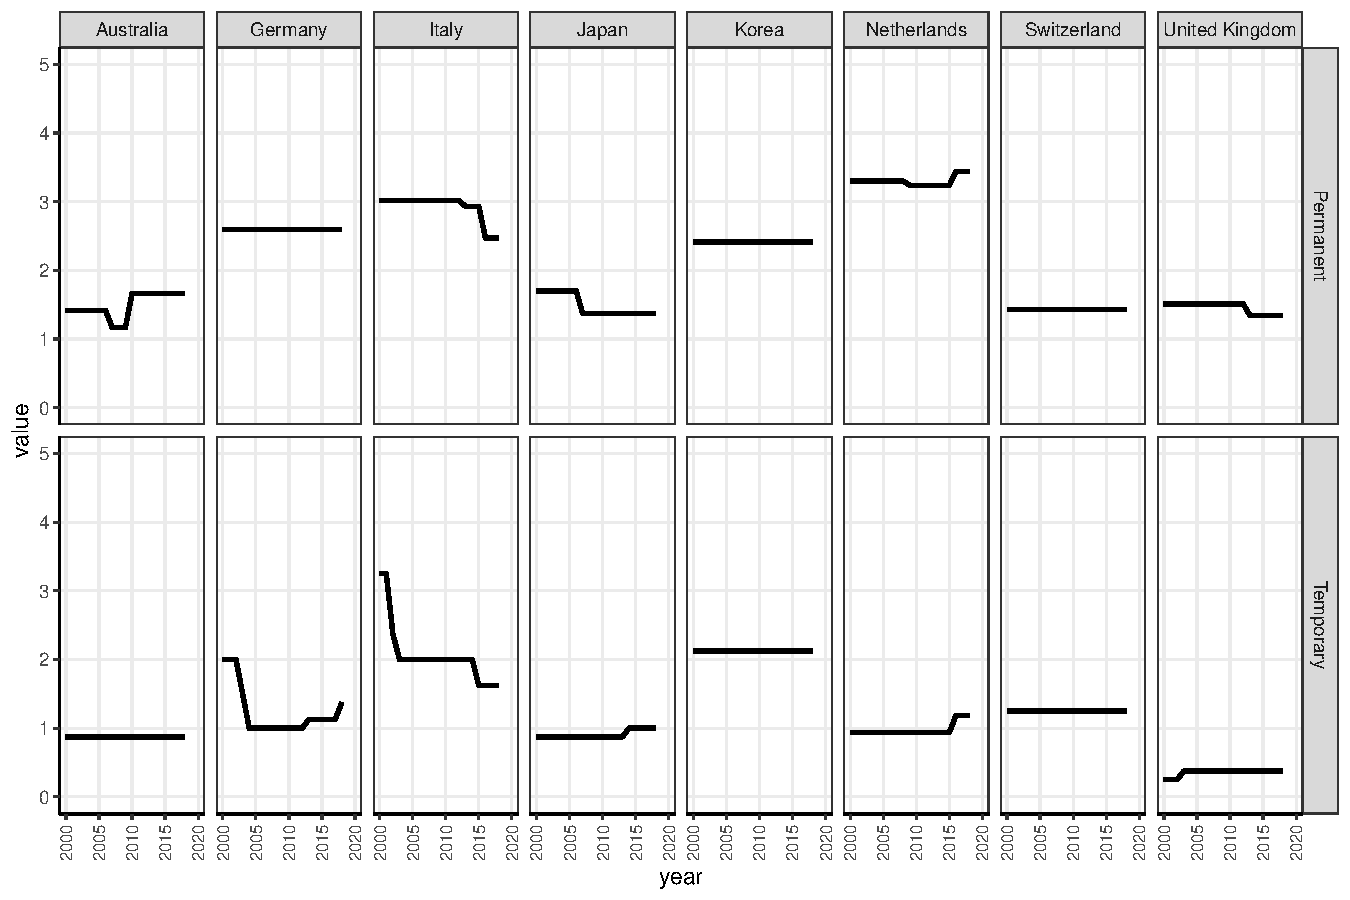
\includegraphics{../../../graphs/descriptives/graph_epl.pdf}}
    \label{graph_epl}
\end{sidewaysfigure}


\begin{sidewaystable}[!h]
    \caption{Country specific frequency and transition counts into and out of temporary employment}
    \centering
    \resizebox{\textwidth}{!}{\begin{tabular}{l>{\raggedright\arraybackslash}p{2.5in}llllllllllllllllll}
   \toprule 
 
\multicolumn{14}{l}{{\bf Panel A:} Sample selection criteria} \\ 

&  & 
\multicolumn{2}{l}{Total (all countries)} &
\multicolumn{2}{l}{Australia} &
\multicolumn{2}{l}{Germany} &
\multicolumn{2}{l}{Italy} &
\multicolumn{2}{l}{Japan} &
\multicolumn{2}{l}{Korea} &
\multicolumn{2}{l}{Netherlands} &
\multicolumn{2}{l}{Switzerland} &
\multicolumn{2}{l}{United Kingdom}
\\  
 
 
\multicolumn{1}{l}{Step} & 
\multicolumn{1}{l}{Description} 
& n & $\Delta$
& n & $\Delta$
& n & $\Delta$
& n & $\Delta$
& n & $\Delta$
& n & $\Delta$
& n & $\Delta$
& n & $\Delta$
& n & $\Delta$
\\ 
\cmidrule(lr){1-2}
\cmidrule(lr){3-4}
\cmidrule(lr){5-6}
\cmidrule(lr){7-8}
\cmidrule(lr){9-10}
\cmidrule(lr){11-12}
\cmidrule(lr){13-14}
\cmidrule(lr){15-16}
\cmidrule(lr){17-18}
\cmidrule(lr){19-20}
\\[-1.8ex]  
 
0 & Raw data & 415,771 &  & 31,951 &  & 91,693 &  & 100,847 &  & 10,499 &  & 24,491 &  & 14,458 &  & 34,469 &  & 107,363 &  \\ 
  1 & Panel years between 2000 and 2018 & 367,032 & -12\% & 31,951 & 0\% & 83,722 & -9\% & 68,012 & -33\% & 10,499 & 0\% & 23,515 & -4\% & 14,458 & 0\% & 34,469 & 0\% & 100,406 & -6\% \\ 
  2 & Prime age (25 - 54) & 210,900 & -43\% & 19,431 & -39\% & 52,198 & -38\% & 33,724 & -50\% & 6,315 & -40\% & 16,089 & -32\% & 9,693 & -33\% & 17,205 & -50\% & 56,245 & -44\% \\ 
  3 & Labour force participant (employed or unemployed) & 157,370 & -25\% & 15,881 & -18\% & 38,538 & -26\% & 25,547 & -24\% & 4,787 & -24\% & 10,980 & -32\% & 7,461 & -23\% & 9,251 & -46\% & 44,925 & -20\% \\ 
  4 & Non missing education or gender & 155,535 & -1\% & 15,875 & 0\% & 37,635 & -2\% & 25,547 & 0\% & 4,767 & 0\% & 10,978 & 0\% & 7,449 & 0\% & 9,251 & 0\% & 44,033 & -2\% \\ 
  5 & Hourly wages within the top/bottom 0.005 percentile & 154,743 & -1\% & 15,817 & 0\% & 37,454 & 0\% & 25,336 & -1\% & 4,754 & 0\% & 10,943 & 0\% & 7,404 & -1\% & 9,168 & -1\% & 43,867 & 0\% \\ 
  6 & Sample A: At least 3 observations & 79,148 & -49\% & 10,598 & -33\% & 20,972 & -44\% & 3,678 & -85\% & 3,179 & -33\% & 7,311 & -33\% & 2,418 & -67\% & 5,303 & -42\% & 25,689 & -41\% \\ 
  7 & Sample B: + always employed & 73,189 & -8\% & 10,072 & -5\% & 18,302 & -13\% & 3,449 & -6\% & 3,079 & -3\% & 7,103 & -3\% & 2,320 & -4\% & 5,153 & -3\% & 23,711 & -8\% \\ 
   
\hline \\[-1.8ex]  
 
\multicolumn{14}{l}{{\bf Panel B:} Data sets by event type (if treated, must be employed after treatment)} \\ 

& 
& \# & \%
& \# & \%
& \# & \%
& \# & \%
& \# & \%
& \# & \%
& \# & \%
& \# & \%
& \# & \%
\\ 
\cmidrule(lr){1-2}
\cmidrule(lr){3-4}
\cmidrule(lr){5-6}
\cmidrule(lr){7-8}
\cmidrule(lr){9-10}
\cmidrule(lr){11-12}
\cmidrule(lr){13-14}
\cmidrule(lr){15-16}
\cmidrule(lr){17-18}
\cmidrule(lr){19-20}
\\[-1.8ex]  
 
A & Unmp $\rightarrow$ perm & 3,670 & 5\% & 452 & 4\% & 1,036 & 5\% & 48 & 1\% & 155 & 5\% & 382 & 5\% & 21 & 1\% & 167 & 3\% & 1,409 & 5\% \\ 
  A & Unmp $\rightarrow$ temp & 1,268 & 2\% & 148 & 1\% & 623 & 3\% & 41 & 1\% & 34 & 1\% & 40 & 1\% & 36 & 1\% & 35 & 1\% & 311 & 1\% \\ 
  B & Temp $\rightarrow$ perm & 9,063 & 12\% & 2,270 & 23\% & 2,757 & 15\% & 291 & 8\% & 227 & 7\% & 893 & 13\% & 260 & 11\% & 360 & 7\% & 2,005 & 8\% \\ 
  B & Perm $\rightarrow$ temp & 6,800 & 9\% & 1,992 & 20\% & 1,559 & 9\% & 237 & 7\% & 232 & 8\% & 822 & 12\% & 198 & 9\% & 250 & 5\% & 1,510 & 6\% \\ 
   \bottomrule \\[-1.8ex] \multicolumn{20}{p{12in}}{Note: n - is unique observations.  $\Delta$ - is difference in n from previous step.  \# - is unique n who experienced at least 1 event.  \% - is percent who experienced an event.} 
\end{tabular}
}
    \label{table_sample_filter_steps_country_transitions}
\end{sidewaystable}

\begin{sidewaystable}[!h]
    \caption{Why are the number of unemployment exits so small in table \ref{table_sample_filter_steps_country_transitions}?}
    \centering
    \resizebox{\textwidth}{!}{\begin{tabular}{l>{\raggedright\arraybackslash}p{2in}llllllllllllllllll}
   \\[-1.8ex]\hline\hline \\ 
 [-1.8ex]
\multicolumn{20}{l}{{\bf Panel A:} Sample selection criteria} \\ 

&  & 
\multicolumn{2}{l}{Total (all countries)} &
\multicolumn{2}{l}{Australia} &
\multicolumn{2}{l}{Germany} &
\multicolumn{2}{l}{Italy} &
\multicolumn{2}{l}{Japan} &
\multicolumn{2}{l}{Korea} &
\multicolumn{2}{l}{Netherlands} &
\multicolumn{2}{l}{Switzerland} &
\multicolumn{2}{l}{United Kingdom}
\\  
 
 
\multicolumn{1}{l}{Step} & 
\multicolumn{1}{l}{Description} 
& n & $\Delta$
& n & $\Delta$
& n & $\Delta$
& n & $\Delta$
& n & $\Delta$
& n & $\Delta$
& n & $\Delta$
& n & $\Delta$
& n & $\Delta$
\\ 
\cmidrule(lr){1-2}
\cmidrule(lr){3-4}
\cmidrule(lr){5-6}
\cmidrule(lr){7-8}
\cmidrule(lr){9-10}
\cmidrule(lr){11-12}
\cmidrule(lr){13-14}
\cmidrule(lr){15-16}
\cmidrule(lr){17-18}
\cmidrule(lr){19-20}
\\[-1.8ex]  
 
1 & Total unemployment events (From data set A) & 14,450 &  & 1,917 &  & 5,562 &  & 335 &  & 364 &  & 980 &  & 184 &  & 531 &  & 4,577 &  \\ 
  2 & Must exit unemployment & 6,463 & -55\% & 1,060 & -45\% & 2,079 & -63\% & 145 & -57\% & 212 & -42\% & 478 & -51\% & 90 & -51\% & 256 & -52\% & 2,143 & -53\% \\ 
  3 & Employed at least 1 period after exit (within 5 years) & 4,847 & -25\% & 592 & -44\% & 1,608 & -23\% & 86 & -41\% & 184 & -13\% & 419 & -12\% & 56 & -38\% & 199 & -22\% & 1,703 & -21\% \\ 
   
\hline \\[-1.8ex]  
 
\multicolumn{20}{l}{{\bf Panel B:} Frequency, by event type} \\ 

& 
&  \# & \%
&  \# & \%
&  \# & \%
&  \# & \%
&  \# & \%
&  \# & \%
&  \# & \%
&  \# & \%
&  \# & \%
\\ 
\cmidrule(lr){1-2}
\cmidrule(lr){3-4}
\cmidrule(lr){5-6}
\cmidrule(lr){7-8}
\cmidrule(lr){9-10}
\cmidrule(lr){11-12}
\cmidrule(lr){13-14}
\cmidrule(lr){15-16}
\cmidrule(lr){17-18}
\cmidrule(lr){19-20}
\\[-1.8ex]  
 
 & Unmp $\rightarrow$ temp & 1,268 & 26\% & 148 & 25\% & 623 & 39\% & 41 & 48\% & 34 & 18\% & 40 & 10\% & 36 & 64\% & 35 & 18\% & 311 & 18\% \\ 
   & Unmp $\rightarrow$ perm & 3,670 & 76\% & 452 & 76\% & 1,036 & 64\% & 48 & 56\% & 155 & 84\% & 382 & 91\% & 21 & 38\% & 167 & 84\% & 1,409 & 83\% \\ 
   & U $\rightarrow$ P \& U $\rightarrow$ T & 91 &  & 8 &  & 51 &  & 3 &  & 5 &  & 3 &  & 1 &  & 3 &  & 17 &  \\ 
   \hline \\[-1.8ex] \multicolumn{20}{p{12in}}{Notes: n - is unique observations.  
               $\Delta$ - is difference in n from previous step.  
               \# - is number of transitions.  
               \% - is percent of total transitions from step 3. 
               \% is more than 100\% because some individuals experience both a transition from Unmp to Perm and Unmp to Temp.} 
\end{tabular}
}
    \label{table_sample_unmp_steps_contyp}
\end{sidewaystable}

\begin{sidewaystable}[!h]
    \caption{Panel attrition for individuals who experience unemployment}
    \centering
    \resizebox{\textwidth}{!}{\begin{tabular}{llllllllllllllllll}
   \toprule 
 
&&
\multicolumn{2}{l}{Australia} &
\multicolumn{2}{l}{Germany} &
\multicolumn{2}{l}{Italy} &
\multicolumn{2}{l}{Japan} &
\multicolumn{2}{l}{Korea} &
\multicolumn{2}{l}{Netherlands} &
\multicolumn{2}{l}{Switzerland} &
\multicolumn{2}{l}{United Kingdom}
\\  
 
 
\multicolumn{1}{l}{Periods} & 
\multicolumn{1}{l}{Description} 
& n & $\Delta$
& n & $\Delta$
& n & $\Delta$
& n & $\Delta$
& n & $\Delta$
& n & $\Delta$
& n & $\Delta$
& n & $\Delta$
\\ 
\cmidrule(lr){1-2}
\cmidrule(lr){3-4}
\cmidrule(lr){5-6}
\cmidrule(lr){7-8}
\cmidrule(lr){9-10}
\cmidrule(lr){11-12}
\cmidrule(lr){13-14}
\cmidrule(lr){15-16}
\cmidrule(lr){17-18}
\\[-1.8ex]  
 
 & Total observations & 16,260 &  & 41,396 &  & 25,784 &  & 5,075 &  & 11,610 &  & 8,082 &  & 10,745 &  & 46,395 &  \\ 
  1 period & Ever unemployed & 2,950 & -82\% & 11,274 & -73\% & 1,311 & -95\% & 542 & -89\% & 1,547 & -87\% & 695 & -91\% & 894 & -92\% & 8,422 & -82\% \\ 
  2 periods & + Exit unemployment & 1,442 & -51\% & 3,442 & -69\% & 166 & -87\% & 288 & -47\% & 686 & -56\% & 174 & -75\% & 460 & -49\% & 2,457 & -71\% \\ 
  3 periods & + 1 period after exit & 1,137 & -21\% & 2,338 & -32\% & 69 & -58\% & 236 & -18\% & 572 & -17\% & 78 & -55\% & 342 & -26\% & 1,771 & -28\% \\ 
   \bottomrule  
\end{tabular}
}
    \label{descriptives_table_unemployment}
\end{sidewaystable}


\begin{table}[!h]
    \caption{Sample filter steps comparing LISS and LSP from the Netherlands}
    \centering
    \resizebox{\textwidth}{!}{\begin{tabular}{llllll}
   \toprule 
 [-1.8ex]
\multicolumn{6}{l}{{\bf Panel A:} Sample selection criteria} \\ 

&  & 
\multicolumn{2}{l}{NE - LSP} &
\multicolumn{2}{l}{NE - LISS}
\\  
 
 
\multicolumn{1}{l}{Step} & 
\multicolumn{1}{l}{Description} 
& n & $\Delta$
& n & $\Delta$
\\ 
\cmidrule(lr){1-2}
\cmidrule(lr){3-4}
\cmidrule(lr){5-6}
\\[-1.8ex]  
 
0 & Raw data & 14,458 &  & 13,121 &  \\ 
  1 & Panel years between 2000 and 2018 & 14,458 & 0\% & 12,976 & -1\% \\ 
  2 & Prime age (25 - 54) & 9,693 & -33\% & 6,641 & -49\% \\ 
  3 & Labour force participant (employed or unemployed) & 8,757 & -10\% & 5,505 & -17\% \\ 
  4 & Unemployed or employed with contract type & 8,082 & -8\% & 4,981 & -10\% \\ 
  5 & Unemployed or employed with wages & 7,765 & -4\% & 3,814 & -23\% \\ 
  6 & Unemployed or employed with monthly hours between 40 and 320 & 7,461 & -4\% & 3,758 & -1\% \\ 
  7 & Non missing education or gender & 7,449 & 0\% & 3,746 & 0\% \\ 
  8 & Hourly wages within the top/bottom 0.005 percentile & 7,404 & -1\% & 3,720 & -1\% \\ 
  9 & Sample A: At least 3 observations & 2,418 & -67\% & 1,432 & -62\% \\ 
  10 & Sample B: + always employed & 2,325 & -4\% & 1,313 & -8\% \\ 
   
\hline \\[-1.8ex]  
 
\multicolumn{6}{l}{{\bf Panel B:} Data sets by event type (if treated, must be employed after treatment)} \\ 

& 
& \# & \%
& \# & \%
\\ 
\cmidrule(lr){3-4}
\cmidrule(lr){5-6}
\\[-1.8ex]  
 
A & Unmp $\rightarrow$ perm & 19 & 1\% & 12 & 1\% \\ 
  A & Unmp $\rightarrow$ temp & 32 & 1\% & 8 & 1\% \\ 
  B & Temp $\rightarrow$ perm & 174 & 7\% & 63 & 5\% \\ 
  B & Perm $\rightarrow$ temp & 182 & 8\% & 44 & 3\% \\ 
   \bottomrule \\[-1.8ex] \multicolumn{6}{p{7in}}{Notes: In Panel A: n - is unique observations and $\Delta$ - is difference in n from previous step.  In Panel B: \# - is unique n who experienced at least 1 event and \% - is percent who experienced an event.} 
\end{tabular}
}
    \label{table_sample_filter_steps_country_NE}
\end{table}

%%%%%%%%%%%%%%%%%%%%%%%%%%%%%%%%%%%%%%%%%%
%%%%%%%%%%%%%%%%%%%%%%%%%%%%%%%%%%%%%%%%%%
%%%%%%%%%%%%%%%%%%%%%%%%%%%%%%%%%%%%%%%%%%
%%%%%%%%%%%%%%%%%%%%%%%%%%%%%%%%%%%%%%%%%%
\clearpage
\section{Appendix: Multiple events}\label{appendix:multiple}
\setcounter{figure}{0}    
\setcounter{table}{0}    
\renewcommand*\thetable{\Alph{section}.\arabic{table}}
\renewcommand*\thefigure{\Alph{section}.\arabic{figure}}
\renewcommand{\theHfigure}{\Alph{section}.\arabic{table}}
\renewcommand{\theHtable}{\Alph{section}.\arabic{figure}}

Let us imagine employment status for one individual in 6 periods of time looks like this: T (50) $\rightarrow$ P (90) $\rightarrow$T (110) $\rightarrow$ P (130) $\rightarrow$ T (140) $\rightarrow$ T (150), as shown in table \ref{table_compare_transformed_data_original} and figure \ref{graph_descriptives_multiple_events_num}.  In this case, we observe four distinct events T $\rightarrow$ P ($\times 2$), and P $\rightarrow$ T ($\times 2$).  

\begin{itemize} 
    \item T $\rightarrow$ P ($\times 2$)
    \begin{itemize} 
        \item $\hat{\beta} event^{T \rightarrow P (1)}_{it} = 40$ 
        \item $\hat{\beta} event^{T \rightarrow P (2)}_{it} = 20$
        \item The average of the two events: $\hat{\beta} event^{T \rightarrow P}_{it} = 30$
    \end{itemize}
    \item P $\rightarrow$ T ($\times 2$)
    \begin{itemize} 
        \item $\hat{\beta} event^{P \rightarrow T (1)}_{it} = 20$
        \item $\hat{\beta} event^{P \rightarrow T (2)}_{it} = 10$
        \item The average of the two events: $\hat{\beta} event^{P \rightarrow T}_{it} = 15$
    \end{itemize}
\end{itemize}

In order to model each of the four distinct events, we must transform the data from person, year data into person, event, year data.  The steps are as follows:

\begin{enumerate}  
    \item For each individual, filter one row per individual, transition at the year the transition occurs ($t_0$).  The result is four rows, one for each event.  This is data frame $A$.
    \item Create 3 variables in data frame $A$:
    \begin{enumerate}
        \item $eventyear=year$ is the year the transition took place  
        \item $transeq$ is cumulative to identify each individual, transition
        \item $eventtime=0$ is for period the transition took place
    \end{enumerate}  
    \item Create data frame $B$ by selecting five variables: $pid$, $year$, $transseq$, $eventyear$, and $eventtime$, i.e. drop $wages$.  
    \item For each individual, transition ($transseq$), we append rows for $eventtime$ four years before ($-$) and six years after the transition ($+$).  Recode $year=year+eventtime$  
    \item Create data frame $C$ by merging data frame $B$ with $A$, by $pid$, $year$ 
    \item In data frame $C$, create a new identifier for each individual, transition sequence ($pidseq$) by multiplying $pid \times transseq \times 100$.  We multiply by 100 to ensure no duplicate $pidseq$
    \item We code the pre/post timing of the distinct events ($event\_p\_t\_time$ and $event\_t\_p\_time$) and create a positive value by adding 3 ($event\_p\_t\_time\_pos$ and $event\_t\_p\_time\_pos$)
\end{enumerate}  

The result is a new data frame with 24 rows: six observations per transition, as shown in table \ref{table_compare_transformed_data_transformed}.  Though not shown, the final steps in the process are to transform the $eventtime\_pos$ for each distinct transition into dummies (reference is year before event, i.e. 2).  

The transformed data do not alter the findings obtained by applying FE and FEIS models to untransformed data, as shown in table \ref{table_compare_transformed_data_original}.  As in the paper, we note that while there are alternative solutions to modeling both transitions simultaneously.  For example, Allison \citeyearpar{allison_asymmetric_2019} codes a transition from one status to another as a permanent and absorbing event.  While this solution is appropriate for some types of events, this is not an appropriate solution for employment status, which changes over time.  However, as shown in figure \ref{graph_sensitivity_single_multiple_events}, if we followed the Allison solution, estimates from first, single event are similar to estimates from multiple events.  The reason is that most people do not experience multiple events of the same transition, but some do, as shown in figure \ref{graph_descriptives_multiple_events_num}.  


\begin{lstlisting}[language=R]
# Create empty work space

rm(list=ls())

# Load library 

library(tidyverse)

# Step 1: Create data 

df_a <- data.frame(
        pid = c(1,1,1,1,1,1),
        year = c(1,2,3,4,5,6),
        wage = c(50,90,110,130,140,150),
        temp = c(1,0,1,0,1,1),
        perm = c(0,1,0,1,0,0)
)

# Step 2: Identify transitions 

df_b <- df_a %>%
        arrange(pid, year) %>%
        group_by(pid) %>%
        # identify type of transition
        mutate(event_t_p_yes = ifelse(perm == 1 & lag(temp,1) == 1 & row_number()>1, yes = 1, no = NA),
               event_p_t_yes = ifelse(temp == 1 & lag(perm,1) == 1 & row_number()>1, yes = 1, no = NA),
        ) %>%
        ungroup() %>%
        # identify whether trans is whether transition occurred
        mutate(trans = rowSums(select(., contains("event_")), na.rm = TRUE)) %>%
        group_by(pid) %>%
        # transseq is the cumulative count for number of transitions
        mutate(transseq = cumsum(ifelse(is.na(trans), 0, trans))) %>%
        ungroup()

# Step 3: Create new data set, 1 row for each transition at time of transition.  

df_c <- df_b %>%
        filter(trans==1) %>%
        group_by(pid,transseq) %>%
        filter(row_number()==1) %>%
        # identify year transition took place
        mutate(eventtime=0,
               eventyear=year) %>%
        ungroup() %>%
        select(pid, year, transseq, matches("event"))

# Step 4: Generate sequence indicator for years pre/post transition 

df_d <- data.frame()
event <- c(-4,-3,-2,-1,1,2,3,4,5,6)
for (e in event) {
        df_test <- df_c %>%
                # create eventtime for years pre/post transition
                mutate(eventtime=e) 
        df_d <- rbind(df_d,df_test)
}                

# Step 5: Append data frame from step 2 and 3

df_e <- rbind(df_c,df_d) %>%
        arrange(pid,transseq,eventtime) %>%
        mutate(year = year+eventtime) %>% 
        arrange(pid,transseq,year)

# Step 6: Merge wage data

df_f <- merge(df_e,df_a) %>%
        arrange(pid,transseq,year) %>%
        mutate(pidseq=pid*100+transseq) %>%  # new identifier
        select(pid, year, pidseq, transseq, wage, temp, perm, eventyear, eventtime, everything())


# Step 7: Code events

df_g <- df_f %>%
  arrange(pidseq,year) %>%
  group_by(pidseq) %>%
  # temp to perm
  mutate(event_t_p_time = ifelse(event_t_p_yes == 1, yes = year - eventyear, no = 0),
         event_t_p_time = ifelse(event_t_p_time < -2, yes = -3, # lower bound
                                 ifelse(event_t_p_time >= 5, yes = 5, no = event_t_p_time)), # upper bound
         event_t_p_time_pos = ifelse(event_t_p_yes == 1, yes = event_t_p_time + 3, no = 0), # make positive
  ) %>%
  # perm to temp
  mutate(event_p_t_time = ifelse(event_p_t_yes == 1, yes = year - eventyear, no = 0),
         event_p_t_time = ifelse(event_p_t_time < -2, yes = -3, # lower bound
                                 ifelse(event_p_t_time >= 5, yes = 5, no = event_p_t_time)), # upper bound
         event_p_t_time_pos = ifelse(event_p_t_yes == 1, yes = event_p_t_time + 3, no = 0), # make positive
  ) %>%
  replace(is.na(.), 0) %>% 
  ungroup()

# Print original and final data frame
print(df_a)

print(df_g)
\end{lstlisting}


\clearpage

\begin{sidewaysfigure}[!h]
    \caption{Simulation figure: Single individual with multiple events}
    \resizebox{\textwidth}{!}{\includegraphics{../../../support_files/simulation/graphs/graph_compare_transformed_data_paper.pdf}}
    \label{graph_compare_transformed_data}
\end{sidewaysfigure}


\begin{table}[!h]
\rowcolors{2}{gray!50}{gray!10}
\caption{Simulation data: Single individual with multiple events}
\centering
    \begin{tabular}{rrrrr}
  \hline
pid & year & temp & perm & wage \\ 
  \hline
1 & 1 & 1 & 0 & 50 \\ 
  1 & 2 & 0 & 1 & 90 \\ 
  1 & 3 & 1 & 0 & 110 \\ 
  1 & 4 & 0 & 1 & 130 \\ 
  1 & 5 & 1 & 0 & 140 \\ 
  1 & 6 & 1 & 0 & 150 \\ 
   \hline
\end{tabular}

\label{table_compare_transformed_data_original}
\end{table}

\begin{table}[!h]
\rowcolors{2}{gray!50}{gray!10}
\caption{Simulation data: Transformed data}
\centering
    \resizebox{\textwidth}{!}{\begin{tabular}{rrrrrrrrrrrr}
  \hline
pid & year & transseq & temp & perm & wage & eventyear & eventtime & event\_p\_t\_yes & event\_t\_p\_yes & event\_p\_t\_time\_pos & event\_t\_p\_time\_pos \\ 
  \hline
1 & 1 & 1 & 1 & 0 & 50 & 2 & -1 & 0 & 1 & 0 & 2 \\ 
  1 & 2 & 1 & 0 & 1 & 90 & 2 & 0 & 0 & 1 & 0 & 3 \\ 
  1 & 3 & 1 & 1 & 0 & 110 & 2 & 1 & 0 & 1 & 0 & 4 \\ 
  1 & 4 & 1 & 0 & 1 & 130 & 2 & 2 & 0 & 1 & 0 & 5 \\ 
  1 & 5 & 1 & 1 & 0 & 140 & 2 & 3 & 0 & 1 & 0 & 6 \\ 
  1 & 6 & 1 & 1 & 0 & 150 & 2 & 4 & 0 & 1 & 0 & 7 \\ 
  1 & 1 & 2 & 1 & 0 & 50 & 3 & -2 & 1 & 0 & 1 & 0 \\ 
  1 & 2 & 2 & 0 & 1 & 90 & 3 & -1 & 1 & 0 & 2 & 0 \\ 
  1 & 3 & 2 & 1 & 0 & 110 & 3 & 0 & 1 & 0 & 3 & 0 \\ 
  1 & 4 & 2 & 0 & 1 & 130 & 3 & 1 & 1 & 0 & 4 & 0 \\ 
  1 & 5 & 2 & 1 & 0 & 140 & 3 & 2 & 1 & 0 & 5 & 0 \\ 
  1 & 6 & 2 & 1 & 0 & 150 & 3 & 3 & 1 & 0 & 6 & 0 \\ 
  1 & 1 & 3 & 1 & 0 & 50 & 4 & -3 & 0 & 1 & 0 & 0 \\ 
  1 & 2 & 3 & 0 & 1 & 90 & 4 & -2 & 0 & 1 & 0 & 1 \\ 
  1 & 3 & 3 & 1 & 0 & 110 & 4 & -1 & 0 & 1 & 0 & 2 \\ 
  1 & 4 & 3 & 0 & 1 & 130 & 4 & 0 & 0 & 1 & 0 & 3 \\ 
  1 & 5 & 3 & 1 & 0 & 140 & 4 & 1 & 0 & 1 & 0 & 4 \\ 
  1 & 6 & 3 & 1 & 0 & 150 & 4 & 2 & 0 & 1 & 0 & 5 \\ 
  1 & 1 & 4 & 1 & 0 & 50 & 5 & -4 & 1 & 0 & 0 & 0 \\ 
  1 & 2 & 4 & 0 & 1 & 90 & 5 & -3 & 1 & 0 & 0 & 0 \\ 
  1 & 3 & 4 & 1 & 0 & 110 & 5 & -2 & 1 & 0 & 1 & 0 \\ 
  1 & 4 & 4 & 0 & 1 & 130 & 5 & -1 & 1 & 0 & 2 & 0 \\ 
  1 & 5 & 4 & 1 & 0 & 140 & 5 & 0 & 1 & 0 & 3 & 0 \\ 
  1 & 6 & 4 & 1 & 0 & 150 & 5 & 1 & 1 & 0 & 4 & 0 \\ 
   \hline
\end{tabular}
}
\label{table_compare_transformed_data_transformed}
\end{table}

\begin{table}[!h]
    \caption{Parameter estimates using data in table \ref{table_compare_transformed_data_original}, as shown in figure \ref{graph_compare_transformed_data}}
    \centering
    \resizebox{\textwidth}{!}{
\begin{tabular}{l c c c c c c c}
\toprule
 & \multicolumn{2}{c}{FE} & \multicolumn{2}{c}{FEIS} & \multicolumn{3}{c}{FE + IF} \\
\cmidrule(lr){2-3} \cmidrule(lr){4-5} \cmidrule(lr){6-8}
 & Original & Transformed & Original & Transformed & First & First & Multiple \\
\midrule
Temp                     & $2.50$ & $2.50^{***}$ & $-12.39$ & $-12.39^{***}$ &         &         &             \\
                         & $$     & $(0.00)$     & $()$     & $(0.00)$       &         &         &             \\
Event: T $\rightarrow$ P &        &              &          &                & $40.00$ &         & $30.00^{*}$ \\
                         &        &              &          &                & $()$    &         & $(12.38)$   \\
Event: P $\rightarrow$ T &        &              &          &                &         & $20.00$ & $15.00^{*}$ \\
                         &        &              &          &                &         & $()$    & $(6.19)$    \\
\midrule
Num. obs.                & $6$    & $24$         & $6$      & $24$           & $6$     & $6$     & $24$        \\
\bottomrule
\multicolumn{8}{l}{\scriptsize{$^{***}p<0.001$; $^{**}p<0.01$; $^{*}p<0.05$. Note: In FE + IF, pre and post event coefficients are not shown.}}
\end{tabular}
}
    \label{table_compare_transformed_data_output}
\end{table}

\begin{sidewaysfigure}[!h]
    \caption{How many individuals experience multiple events?}
    \resizebox{\textwidth}{!}{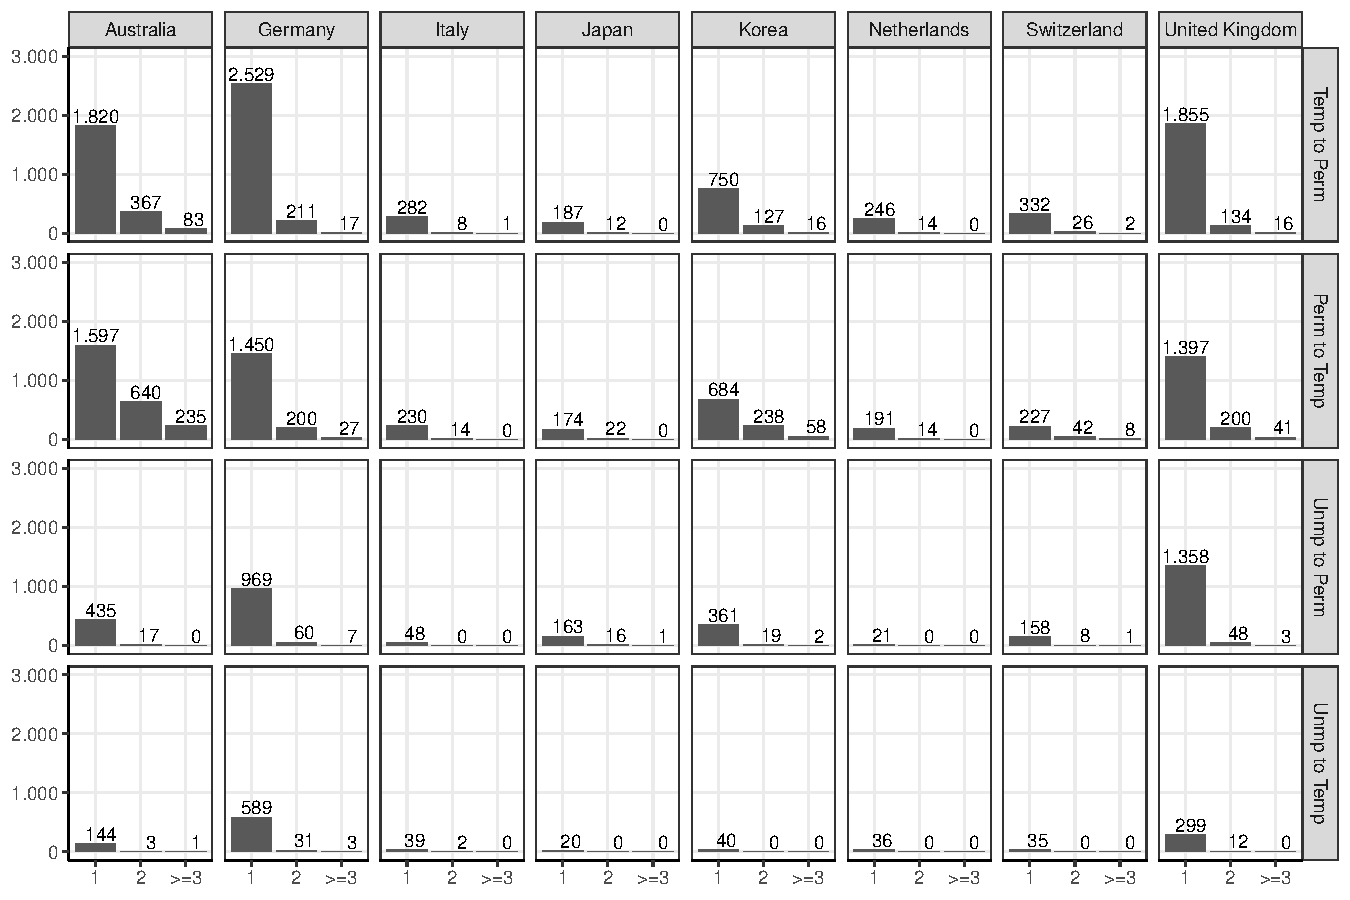
\includegraphics{../../../graphs/descriptives/graph_descriptives_multiple_events_num.pdf}}
    \label{graph_descriptives_multiple_events_num}
\end{sidewaysfigure}

%%%%%%%%%%%%%%%%%%%%%%%%%%%%%%%%%%%%%%%%%%
%%%%%%%%%%%%%%%%%%%%%%%%%%%%%%%%%%%%%%%%%%
%%%%%%%%%%%%%%%%%%%%%%%%%%%%%%%%%%%%%%%%%%
%%%%%%%%%%%%%%%%%%%%%%%%%%%%%%%%%%%%%%%%%%
\clearpage
\section{Appendix: Simulation exercise}\label{appendix:simulation}
\setcounter{figure}{0}    
\setcounter{table}{0}    
\renewcommand*\thetable{\Alph{section}.\arabic{table}}
\renewcommand*\thefigure{\Alph{section}.\arabic{figure}}
\renewcommand{\theHfigure}{\Alph{section}.\arabic{table}}
\renewcommand{\theHtable}{\Alph{section}.\arabic{figure}}

To illustrate our methodological approach, we describe three simple simulations with two individuals in six periods of time, as shown in figure \ref{graph_compare_models_simulation_paper}. In simulation 1, both individuals are the same age and live in the same country. Individual A begins period 1 with a temporary contract earning €100. Individual B begins period 1 with a permanent contract earning €300. In period 4, both individuals switch contracts. Individual A transitions from a temporary to a permanent contract, increasing their wages by €30, to €130. By contrast, individual B transitions from a permanent to a temporary contract, reducing their wages by €30, to €270. Individual-specific counterfactual wages are average wages in a temporary contract. In simulation 1, a temporary contract pays €30 less compared to a permanent contract and -30 is the effect of a temporary contract on wages.

When we apply the FE model \ref{eq:model_fe} to simulation 1, the $\beta$ coefficient for temporary employment is -30, which is the correct effect of a temporary contract on wages, as shown in table \ref{table_compare_models_simulation_paper}.\footnote{$-30 = \frac{(\text{Ind. A} + \text{Ind. B}) \cdot (\text{Avg. wages in Temp} - \text{Avg. wages in Perm})}{2 \text{ individuals}} = \frac{(270-300) + (100-130)}{2} = \frac{(-30) + (-30)}{2} = \frac{-60}{2}$}

Next, let us build on this simulation to include non-parallel trends.  In simulation 2, we assume that individual A, who transitions from a temporary to a permanent contract has a higher wage trajectory, than individual B, who transitions from a permanent to a temporary contract.  The only difference between simulation 1 and simulation 2 is that individual A increases their wages by €20 in each period of time.  Individual B's wages do not change.

Despite the distinct wage trajectories, a temporary contract still pays €30 less than a counterfactual permanent contract assuming trends remained the same.  Therefore, just as in simulation 1, the effect of a temporary contract on wages is still -30.  However, as shown in table 2, when we apply the FE model to simulation 2, the $\beta$  coefficient for temporary employment is -60,\footnote{$-60 = \frac{(\text{Ind. A} + \text{Ind. B}) \cdot (\text{Avg. wages in Temp} - \text{Avg. wages in Perm})}{2 \text{ individuals}} = \frac{(120-210) + (270-300)}{2} = \frac{(-90) + (-30)}{2} = \frac{-120}{2}$} which incorrectly identifies that the effect of a temporary contract on wages because it does not account for the distinct wage trajectories of the two individuals.  

To account for non-parallel trends, we extend model \ref{eq:model_fe} into a random trend model by adding individual-specific linear outcome trends, i.e. interaction terms between a continuous variable for age with the fixed effect for individual ($\alpha_i age_{it}$).  This is referred to as a fixed effects individual slopes (FEIS) estimator  \citep{ludwig_is_2018}, as shown in model \ref{eq:model_feis}.  Data are detrended by subtracting estimated individual linear trend for each variable. This eliminates both individual heterogeneity in levels ($\alpha_i$) and slopes ($\alpha_i age_{it}$). Hence, the FEIS estimator rests on a weaker exogeneity assumption than the FE estimator as it allows for confounding by time-constant variables that lead to linear trends in the outcome variable. When we apply the FEIS estimator to simulation 1 or 2, the $\beta$ coefficient for temporary employment is -30, which is the average difference between actual and counterfactual wages if trends remained the same. 

% The methodological approach used in model \ref{eq:model_feis} follows Brüderl and Ludwig \citeyearpar{ludwig_is_2018}, who cite Wooldridge \citeyearpar[pp. 377–81]{wooldridge_econometric_2010}, but FEIS also has a rich history in the literature examining the consequences of unemployment \citep{jacobson_earnings_1993,stevens_persistent_1997}. 

The issue is that neither the FE nor FEIS models correctly distinguish between asymmetric effect of two distinct events: the positive effect of a transition from temporary into permanent (T $\rightarrow$ P) and the negative effect of a transition from permanent into temporary (P $\rightarrow$ T).  Standard FE estimators must not be interpreted according to the estimation equation, but in line with the structural model that defines the wage effect of having a temporary versus permanent contract \citep{an_causal_2017,wooldridge_econometric_2010}.   The problem is that standard FE models are agnostic with respect to the direction and timing of the transition. Instead, standard FE models only compares average wages when an individual has a temporary contract relative to average wages when that same individual has a permanent contract.  This is still true in standard FEIS models, even if FEIS models do control for differences in individual slopes. 

When we apply the AFE + DIF model \ref{eq:model_afe_temp} to simulation 2, the $\beta$ coefficient for the event T $\rightarrow$ P in period 4 is +50 and the comparable $\beta$ coefficient for the event P $\rightarrow$ T is -30.  The AFE + DIF model classifies the effect of a given transition as the raw, or unadjusted difference in wages between period 4, the year the transition takes place, and period 3, the year before.   

Therefore, unlike the FEIS model \ref{eq:model_feis}, the FE + DIF model  \ref{eq:model_afe_temp} does account for the asymmetric effect of the two events.  The FE + DIF also controls for individual-specific wage trends, but not in the same way as FEIS.  While FEIS assumes that a wage trend's slope or direction is the linear parameter for individual slopes, AFE + DIF makes no assumptions about a wage trend's slope or direction.  We see this as an advantage.  


\begin{sidewaysfigure}[!h]
    \caption{Simulation data}
    \resizebox{\textwidth}{!}{\includegraphics{../../../support_files/simulation/graphs/graph_compare_models_simulation_paper.pdf}}
    \label{graph_compare_models_simulation_paper}
\end{sidewaysfigure}

\begin{table}[!h]
    \caption{Parameter estimates}
    \centering
    \resizebox{\textwidth}{!}{
\begin{tabular}{l c c c c c c c c c}
\toprule
 & \multicolumn{3}{c}{Simulation 1} & \multicolumn{3}{c}{Simulation 2} & \multicolumn{3}{c}{Simulation 3} \\
\cmidrule(lr){2-4} \cmidrule(lr){5-7} \cmidrule(lr){8-10}
 & FE & FEIS & AFE + DIF & FE & FEIS & AFE + DIF & FE & FEIS & AFE + DIF \\
\midrule
Temp                     & $-30.00^{***}$ & $-30.00^{***}$ &          & $-60.00$  & $-30.00^{***}$ &          & $-5.00$   & $-5.00$   &          \\
                         & $(0.00)$       & $(0.00)$       &          & $(31.46)$ & $(0.00)$       &          & $(26.22)$ & $(27.64)$ &          \\
Event: T $\rightarrow$ P &                &                & $30.00$  &           &                & $50.00$  &           &           & $30.00$  \\
                         &                &                & $(0.00)$ &           &                & $(0.00)$ &           &           & $(0.00)$ \\
Event: P $\rightarrow$ T &                &                & $-30.00$ &           &                & $-30.00$ &           &           & $20.00$  \\
                         &                &                & $(0.00)$ &           &                & $(0.00)$ &           &           & $(0.00)$ \\
\bottomrule
\multicolumn{10}{l}{\scriptsize{$^{***}p<0.001$; $^{**}p<0.01$; $^{*}p<0.05$. Note: In AFE + DIF, pre and post event coefficients are not shown.}}
\end{tabular}
}
    \label{table_compare_models_simulation_paper}
\end{table}


%%%%%%%%%%%%%%%%%%%%%%%%%%%%%%%%%%%%%%%%%%
%%%%%%%%%%%%%%%%%%%%%%%%%%%%%%%%%%%%%%%%%%
%%%%%%%%%%%%%%%%%%%%%%%%%%%%%%%%%%%%%%%%%%
%%%%%%%%%%%%%%%%%%%%%%%%%%%%%%%%%%%%%%%%%%
\clearpage
\section{Appendix: Raw coefficients}\label{appendix:coefficients}
\setcounter{table}{0}
\setcounter{figure}{0}
\renewcommand*\thetable{\Alph{section}.\arabic{table}}
\renewcommand*\thefigure{\Alph{section}.\arabic{figure}}
\renewcommand{\theHfigure}{\Alph{section}.\arabic{table}}
\renewcommand{\theHtable}{\Alph{section}.\arabic{figure}}

In this appendix section, we provide the estimated coefficients, standard errors and 95\% confidence intervals for figures \ref{graph_contyp} and \ref{graph_unmp}.

\begin{table}[!h]
    \caption{Results from standard fixed effects (FE) model \ref{eq:model_fe} in figure \ref{graph_contyp}}
    \centering
    \begin{tabular}{lrrrr}
   \toprule 
 
country & estimate & std.error & ymin & ymax \\ 

\cmidrule(lr){1-5} 
 
\\[-1.8ex]  
 
Australia & -0.0305 & 0.0055 & -0.0412 & -0.0198 \\ 
  Switzerland & -0.0913 & 0.0126 & -0.1160 & -0.0667 \\ 
  Germany & -0.0779 & 0.0056 & -0.0888 & -0.0670 \\ 
  Japan & -0.0405 & 0.0213 & -0.0822 & 0.0012 \\ 
  Korea & -0.0218 & 0.0072 & -0.0360 & -0.0076 \\ 
  United Kingdom & -0.0311 & 0.0056 & -0.0420 & -0.0201 \\ 
  Netherlands & -0.0187 & 0.0089 & -0.0363 & -0.0012 \\ 
  Italy & -0.2150 & 0.0184 & -0.2511 & -0.1789 \\ 
   \bottomrule  
\end{tabular}

    \label{beta_coef_contyp_fe}
\end{table}

\begin{table}[!h]
    \caption{Results from fixed effects with individual slopes model \ref{eq:model_feis}  (FEIS) in figure \ref{graph_contyp}}
    \centering
    \begin{tabular}{lrrrr}
   \toprule 
 
country & estimate & std.error & ymin & ymax \\ 

\cmidrule(lr){1-5} 
 
\\[-1.8ex]  
 
Australia & -0.0203 & 0.0056 & -0.0313 & -0.0093 \\ 
  Switzerland & -0.0375 & 0.0127 & -0.0624 & -0.0126 \\ 
  Germany & -0.0384 & 0.0059 & -0.0499 & -0.0268 \\ 
  Japan & -0.0324 & 0.0250 & -0.0814 & 0.0165 \\ 
  Korea & -0.0115 & 0.0075 & -0.0263 & 0.0032 \\ 
  United Kingdom & -0.0204 & 0.0060 & -0.0322 & -0.0087 \\ 
  Netherlands & -0.0008 & 0.0108 & -0.0220 & 0.0204 \\ 
  Italy & -0.1737 & 0.0227 & -0.2183 & -0.1292 \\ 
   \bottomrule  
\end{tabular}

    \label{beta_coef_contyp_feis}
\end{table}

\begin{table}[!h]
    \caption{Results from asymmetric fixed effects model \ref{eq:model_afe_temp} (AFE) for T $\rightarrow$ P in figure \ref{graph_contyp}}
    \centering
    \begin{tabular}{lrrrr}
   \toprule 
 
country & estimate & std.error & ymin & ymax \\ 

\cmidrule(lr){1-5} 
 
\\[-1.8ex]  
 
Australia & 0.0626 & 0.0080 & 0.0469 & 0.0783 \\ 
  Switzerland & 0.0796 & 0.0165 & 0.0471 & 0.1120 \\ 
  Germany & 0.0699 & 0.0072 & 0.0558 & 0.0839 \\ 
  Japan & 0.0484 & 0.0295 & -0.0094 & 0.1061 \\ 
  Korea & 0.0225 & 0.0091 & 0.0046 & 0.0403 \\ 
  United Kingdom & 0.0157 & 0.0073 & 0.0014 & 0.0301 \\ 
  Netherlands & 0.0257 & 0.0135 & -0.0007 & 0.0521 \\ 
  Italy & 0.2485 & 0.0310 & 0.1877 & 0.3092 \\ 
   \bottomrule  
\end{tabular}

    \label{beta_coef_contyp_afe_t_p}
\end{table}


\begin{table}[!h]
    \caption{Results from asymmetric fixed effects model \ref{eq:model_afe_temp} (AFE) for P $\rightarrow$ T in figure \ref{graph_contyp}}
    \centering
    \begin{tabular}{lrrrr}
   \toprule 
 
country & estimate & std.error & ymin & ymax \\ 

\cmidrule(lr){1-5} 
 
\\[-1.8ex]  
 
Australia & 0.0332 & 0.0078 & 0.0180 & 0.0484 \\ 
  Switzerland & -0.0164 & 0.0189 & -0.0534 & 0.0206 \\ 
  Germany & 0.0114 & 0.0094 & -0.0071 & 0.0298 \\ 
  Japan & -0.0476 & 0.0364 & -0.1191 & 0.0238 \\ 
  Korea & 0.0125 & 0.0098 & -0.0067 & 0.0318 \\ 
  United Kingdom & -0.0102 & 0.0089 & -0.0277 & 0.0072 \\ 
  Netherlands & -0.0062 & 0.0159 & -0.0373 & 0.0250 \\ 
  Italy & -0.1938 & 0.0319 & -0.2563 & -0.1313 \\ 
   \bottomrule  
\end{tabular}

    \label{beta_coef_contyp_afe_p_t}
\end{table}

\begin{table}[!h]
    \caption{Results from asymmetric fixed effects model \ref{eq:model_afe_unmp} (AFE) for U $\rightarrow$ T in figure \ref{graph_unmp}}
    \centering
    \begin{tabular}{lrrrr}
   \toprule 
 
country & estimate & std.error & ymin & ymax \\ 

\cmidrule(lr){1-5} 
 
\\[-1.8ex]  
 
Australia & 2.8033 & 0.0565 & 2.6925 & 2.9140 \\ 
  Switzerland & 3.3797 & 0.0844 & 3.2142 & 3.5452 \\ 
  Germany & 2.0819 & 0.0185 & 2.0456 & 2.1182 \\ 
  Japan & 6.3739 & 0.0980 & 6.1819 & 6.5659 \\ 
  Korea & 9.0038 & 0.0745 & 8.8578 & 9.1497 \\ 
  United Kingdom & 2.2195 & 0.0274 & 2.1659 & 2.2732 \\ 
  Netherlands & 2.3789 & 0.0568 & 2.2675 & 2.4902 \\ 
  Italy & 1.4463 & 0.0827 & 1.2842 & 1.6084 \\ 
   \bottomrule  
\end{tabular}

    \label{beta_coef_unmp_afe_u_t}
\end{table}

\begin{table}[!h]
    \caption{Results from asymmetric fixed effects model \ref{eq:model_afe_unmp} (AFE) for U $\rightarrow$ P in figure \ref{graph_unmp}}
    \centering
    \begin{tabular}{lrrrr}
   \toprule 
 
country & estimate & std.error & ymin & ymax \\ 

\cmidrule(lr){1-5} 
 
\\[-1.8ex]  
 
Australia & 2.6969 & 0.0336 & 2.6310 & 2.7628 \\ 
  Switzerland & 3.6070 & 0.0270 & 3.5541 & 3.6599 \\ 
  Germany & 2.1758 & 0.0158 & 2.1449 & 2.2067 \\ 
  Japan & 6.4274 & 0.0511 & 6.3271 & 6.5276 \\ 
  Korea & 8.8667 & 0.0215 & 8.8245 & 8.9090 \\ 
  United Kingdom & 2.2420 & 0.0115 & 2.2195 & 2.2645 \\ 
  Netherlands & 2.4243 & 0.0670 & 2.2930 & 2.5556 \\ 
  Italy & 1.9595 & 0.0666 & 1.8290 & 2.0901 \\ 
   \bottomrule  
\end{tabular}

    \label{beta_coef_unmp_afe_u_p}
\end{table}

%%%%%%%%%%%%%%%%%%%%%%%%%%%%%%%%%%%%%%%%%%
%%%%%%%%%%%%%%%%%%%%%%%%%%%%%%%%%%%%%%%%%%
%%%%%%%%%%%%%%%%%%%%%%%%%%%%%%%%%%%%%%%%%%
%%%%%%%%%%%%%%%%%%%%%%%%%%%%%%%%%%%%%%%%%%
\clearpage
\section{Appendix: Sensitivity to sample selection}\label{appendix:sensitivity_sample}
\setcounter{table}{0}
\setcounter{figure}{0}
\renewcommand*\thetable{\Alph{section}.\arabic{table}}
\renewcommand*\thefigure{\Alph{section}.\arabic{figure}}
\renewcommand{\theHfigure}{\Alph{section}.\arabic{table}}
\renewcommand{\theHtable}{\Alph{section}.\arabic{figure}}

In this appendix section, we replicate the main analysis but for several different samples.  

First, we use a sample that includes ages between 16-64 as opposed to a sample that includes ages between 25-54 (as in the paper).  As one can see in figures \ref{graph_post_age_16_64}, results are qualitatively similar with the exception of Switzerland and Japan.  

In Switzerland, in the sample of 16-64, the negative effect of FE and FEIS models are larger than in the sample of 25-54 year olds.  This is explained by a much larger positive effect of a transition from a temporary to a permanent contract, relative to a transition from a permanent to a temporary contract.  To understand why this may be the case, we examined reasons for being in a temporary contract in Switzerland by four age groups: 16-64, 16-54, 25-54 (sample), 25-64, as shown in figure \ref{graph_ch_compare_sample_age}.  The biggest difference in the reason for being in a temporary contract across the four samples is: `Apprenticeship'.  The difference in the results between the samples is explained by the fact that those under the age of 25 are more than 10 times more likely to have a temporary contract that is an apprenticeship, relative to those over the age of 25 (3\% vs. 44\%).  Therefore, those under the age of 25 have a clearly different reason for having a temporary contract than those over the age of 25.  

In Japan, the only difference between the age samples can be seen in the transition from permanent into temporary contract.  In both age samples, wage effects are similar in the year of the transition and 4 years afterward, but differ in between.  For the sample of 25-54 year olds, wage effects in periods 1, 2, and 3 are positive and constant (but not significant).  For the sample of 16-64 year olds, wage effects rise in periods 1, 2, and 3, but remain negative until period 4, when they are positive (but not significant).  Therefore, point estimates for transitions from permanent into temporary contracts remain less positive over time than transition from temporary into permanent contracts, but not negative.  Over time, point estimates increase so that 4 periods after the transition, wage effects are positive, but not significant.  Thus, the qualitative interpretation does not change.

Second, we compared results from a sample requiring at least 3 observations (as in the paper) to a sample requiring at least 2 observations.  There are two reasons why it is necessary to have at least 3 observations.  One is with respect to fixed effects models with individual slopes (FEIS).  FEIS models only include observations with at least 3 periods.  The reason is that in order to control for a trend, one must have at least 3 observations.  Therefore, to compare across models, we select on individuals that are observable in at least three time periods.  The second, related reason is that we are not only interested in the effect of a distinct transition on wages, but we are also interested in the effect of that transition on wages in periods of time after that transition has occurred.  While some limited research has attempted to examine this issue \citep{booth_temporary_2002,mooi-reci_casual_2017}, they have done this by interacting the treatment effect with years of experience.  While the interaction term captures the deviation from the mean of potential experience on wages, this is not the same thing as the effect of temporary employment over time.  

As a result, it is not known the effect of transitions into or out of temporary employment on wages over time.  Only by including three periods of time, including and especially a period after a transition has occurred can we estimate the effect of that transition over time.  However, we have also conducted a sensitivity test where we estimated the results using a 2-year sample.  Obviously, we are only able to compare estimates using the standard FE and the point in time transitions, but results are qualitatively similar.  These graphs are shown in figures \ref{graph_sensitivity_compare_contyp_sample_2_years} and \ref{graph_sensitivity_compare_unmp_sample_2_years}.  

Third, we compare results from a sample requiring at least 10 to 80 hours per week or 20 to 320 hours per month (as in the paper) to a sample requiring at least 5 to 80 hours per week.  Consistent with previous research \citep{barbieri_dual_2018}, our goal is to reduce bias associated with marginal part-timers or extreme full-timers who lie at the ends of the distribution of hours worked.  However, given there is no single definition of hours per week for a given contract, either part-time or full-time within or between countries.  Therefore, we compare results from a sample with 2 definitions of minimum hours worked per week, as shown in figure \ref{graph_post_hours}.  Results are qualitatively similar. 

Fourth, we compare the results for transitions out of unemployment into a temporary or permanent contract for observations that include those who become unemployed after the transition (main sample A) to only observations that remain employed after the transition (sensitivity sample A).  The concern is that those who transition into temporary employment are usually more likely to become unemployed in the following years, which could result in a relatively larger observed declines in wages. If this is the case, then this could mean that the results tell us not so much about wage effects but rather, indirectly, about employment effects of fixed-term work. To address this, we make two comparisons.  One is within the same transition, but between the two samples, as shown in \ref{graph_post_employed_2}.  Results suggest that wage effects are higher for the sensitivity sample compared to the main sample, as we would expect.  The other is within the same sample, but between the two transitions, as shown in figure \ref{graph_post_employed_1}.  The interpretation is that the qualitative finding from the main text remains unchanged: for unemployed workers in most countries, temporary jobs have a similar integrative potential with regard to wages as permanent contracts.  

\begin{sidewaysfigure}
    \caption{Graphical effect of transition on wages over time with different age samples (as compared to figures \ref{graph_contyp_post} and  \ref{graph_unmp_post})}
    \resizebox{\textwidth}{!}{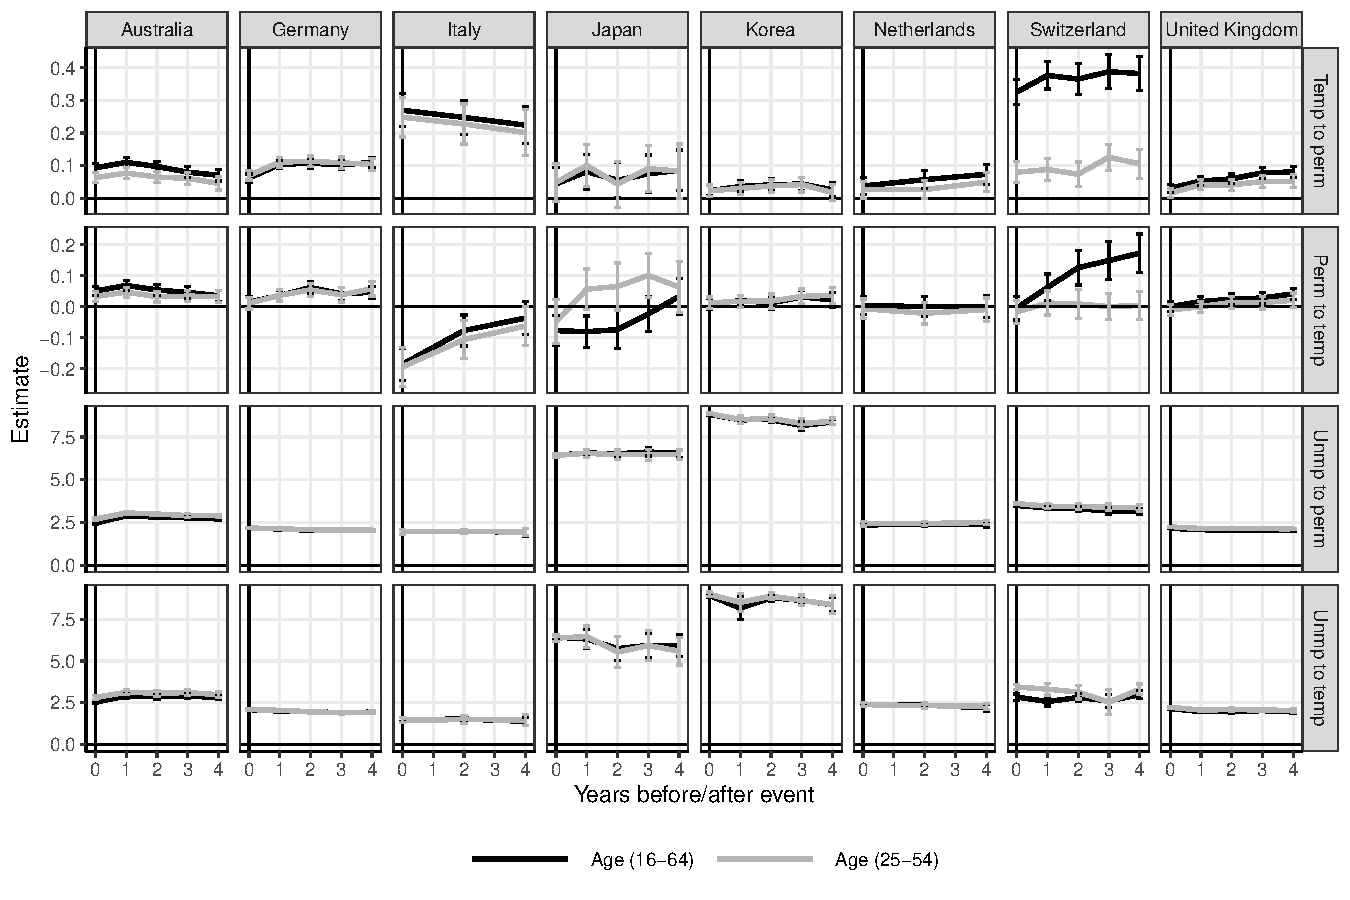
\includegraphics{../../../graphs/age_16_64/graph_sensitivity_age_post.pdf}}
    \label{graph_post_age_16_64}
\end{sidewaysfigure}

\begin{sidewaysfigure}[h!]
    \caption{Switzerland -- Differences in reason for temporary employment by sample age group}
    \resizebox{\textwidth}{!}{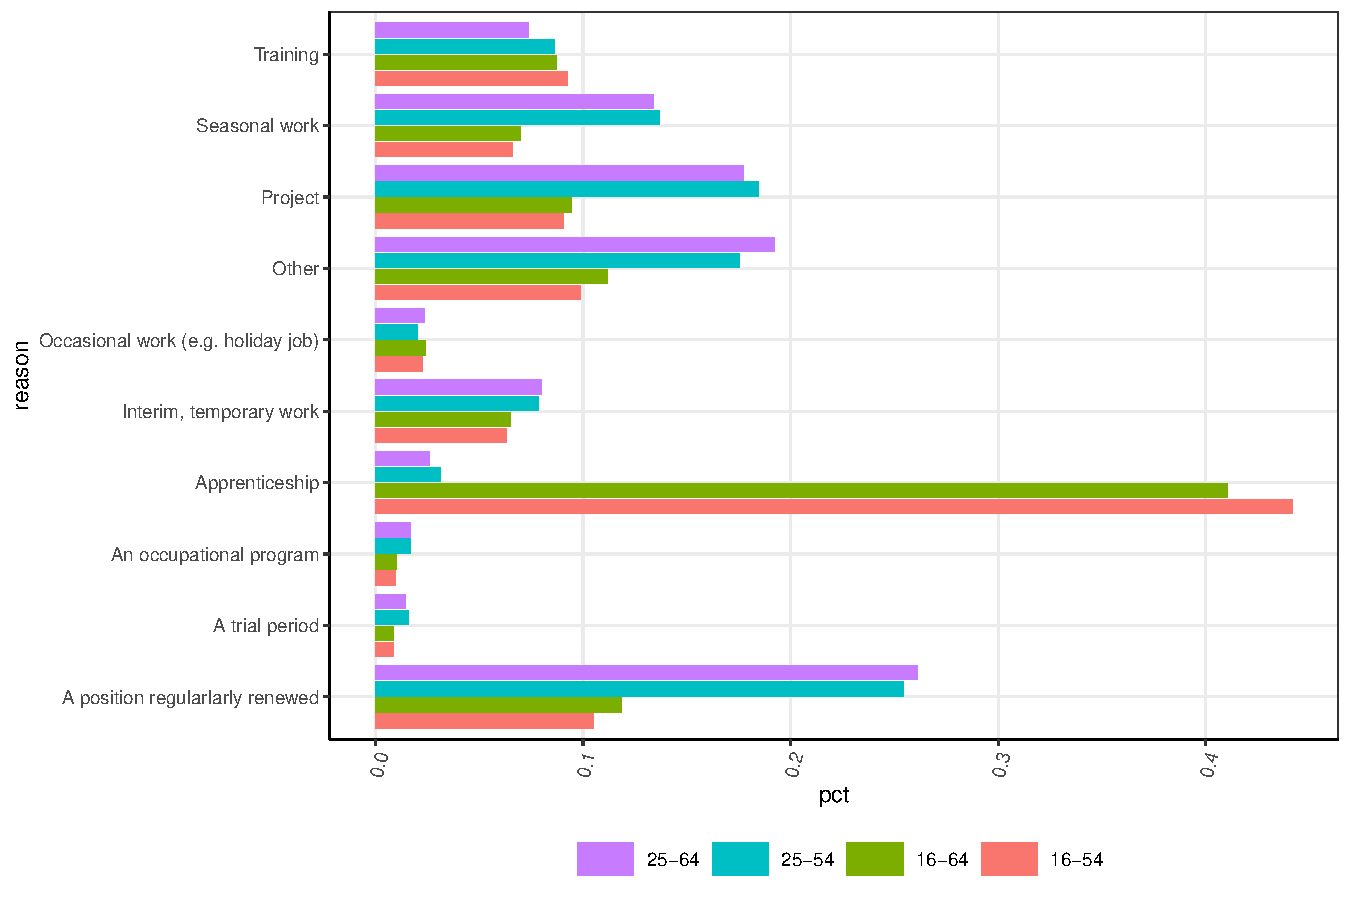
\includegraphics{../../../graphs/age_16_64/graph_ch_compare_sample_age.pdf}}
    \label{graph_ch_compare_sample_age}
\end{sidewaysfigure}

\begin{sidewaysfigure}[!h]
    \caption{Compare sample with at least 3 (as in the paper) vs. 2 observations (compare to figure \ref{graph_contyp})}
    \resizebox{\textwidth}{!}{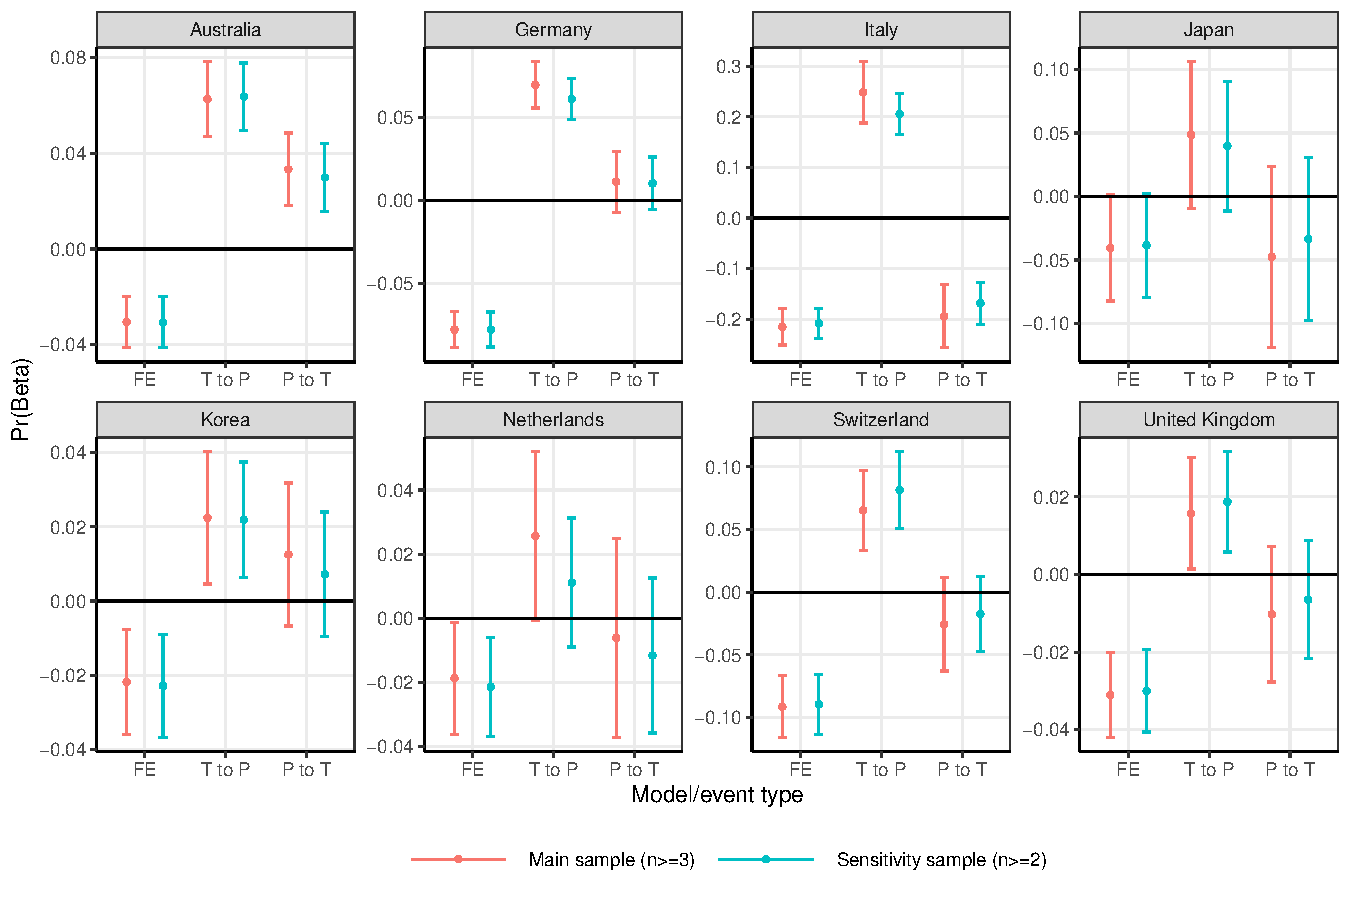
\includegraphics{../../../graphs/sample_2_years/graph_sensitivity_compare_contyp_sample_2_years.pdf}}
    \label{graph_sensitivity_compare_contyp_sample_2_years}
\end{sidewaysfigure}

\begin{sidewaysfigure}[!h]
    \caption{Compare sample with at least 3 (as in the paper) vs. 2 observations (compare to figure \ref{graph_unmp})}
    \resizebox{\textwidth}{!}{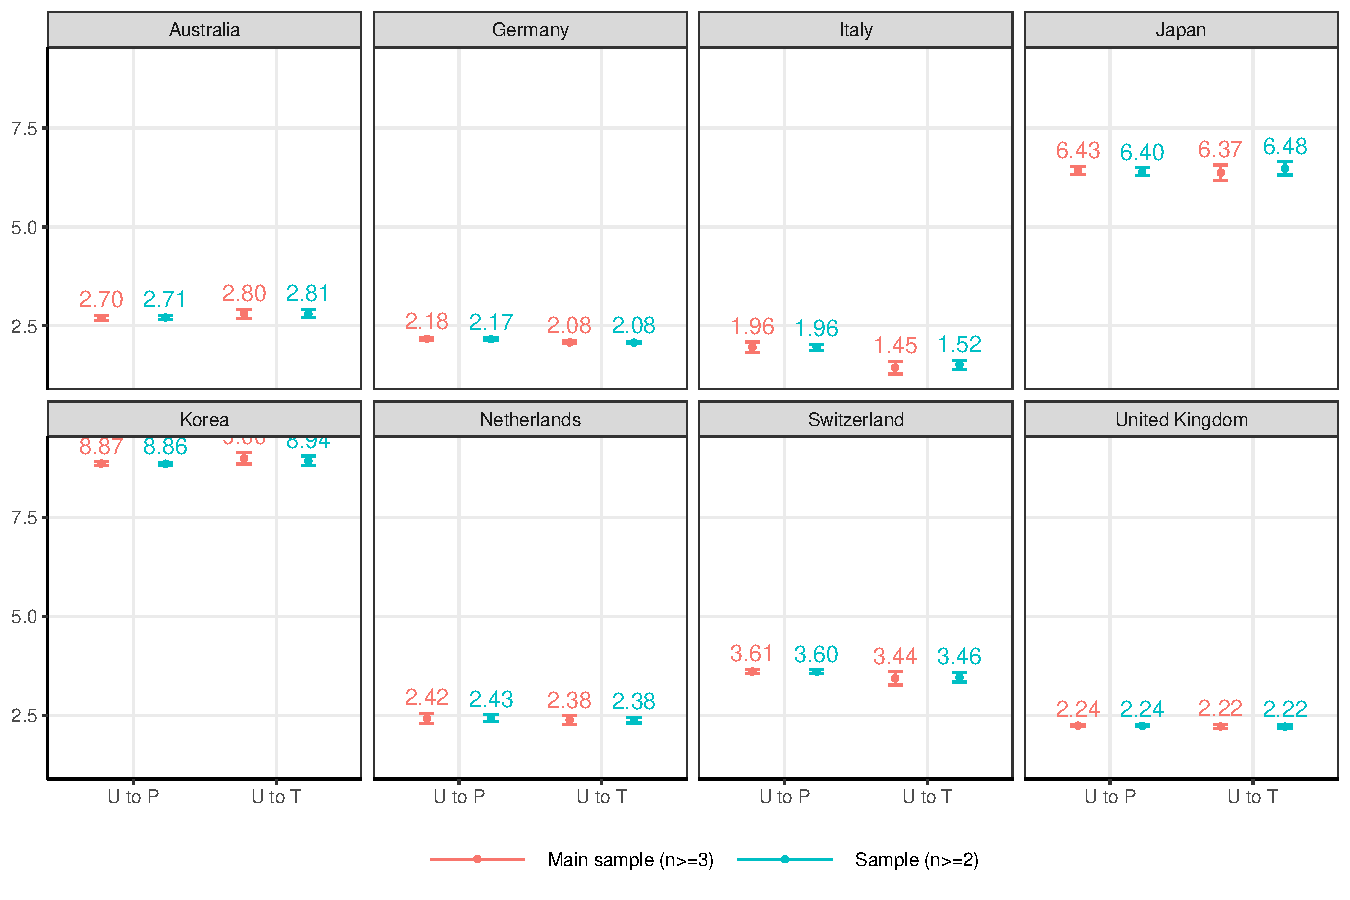
\includegraphics{../../../graphs/sample_2_years/graph_sensitivity_compare_unmp_sample_2_years.pdf}}
    \label{graph_sensitivity_compare_unmp_sample_2_years}
\end{sidewaysfigure}

\begin{sidewaysfigure}[!h]
    \caption{Graphical effect of transition on wages over time with different hours samples (as compared to figures \ref{graph_contyp_post} and  \ref{graph_unmp_post})}
    \resizebox{\textwidth}{!}{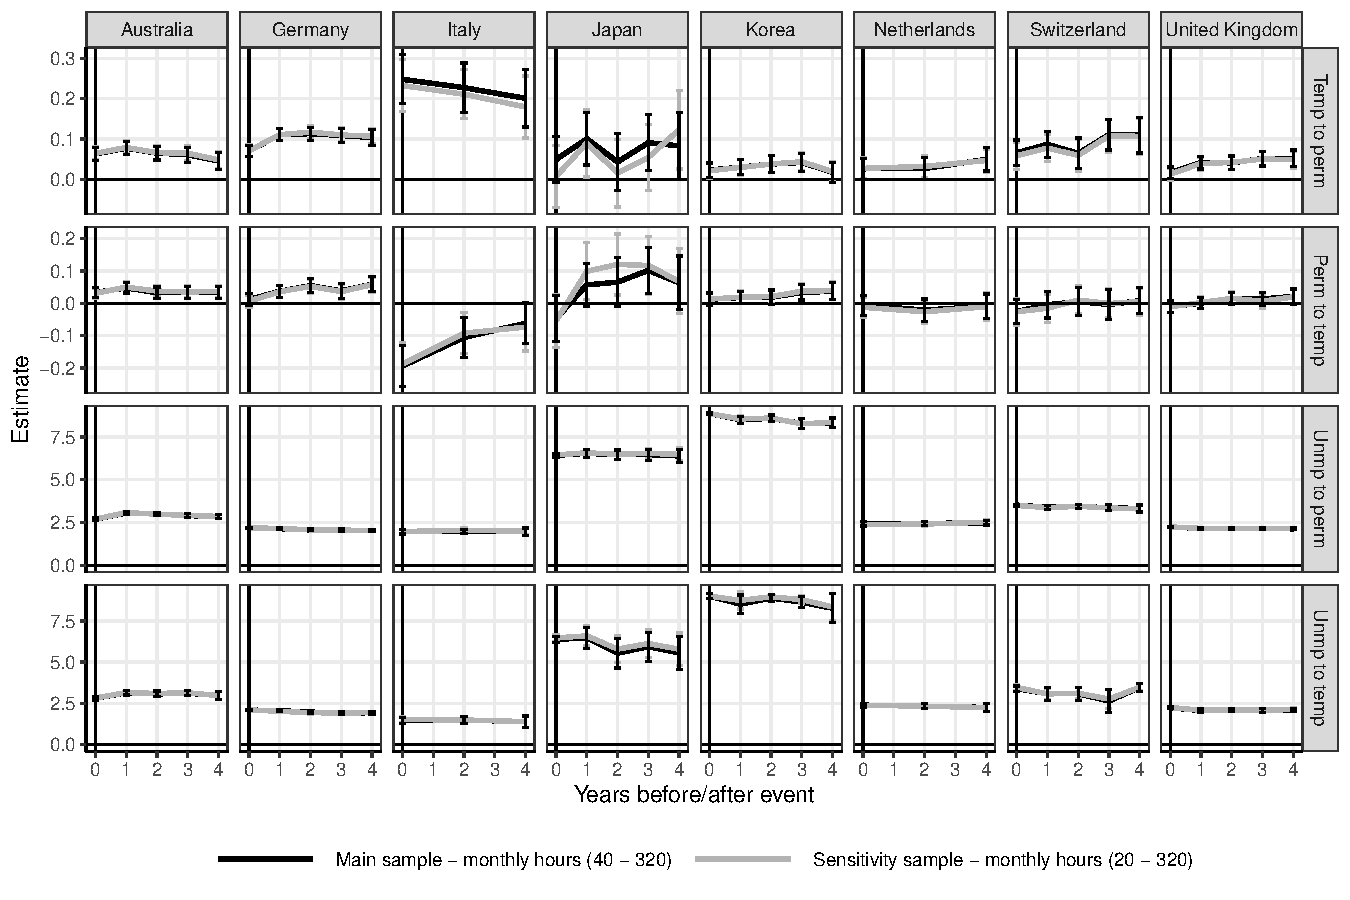
\includegraphics{../../../graphs/hours/graph_sensitivity_hours_post.pdf}}
    \label{graph_post_hours}
\end{sidewaysfigure}

\begin{sidewaysfigure}[!h]
    \caption{Graphical effect of transitions out of unemployment on wages over time with different samples (as compared to figure \ref{graph_unmp_post})}
    \resizebox{\textwidth}{!}{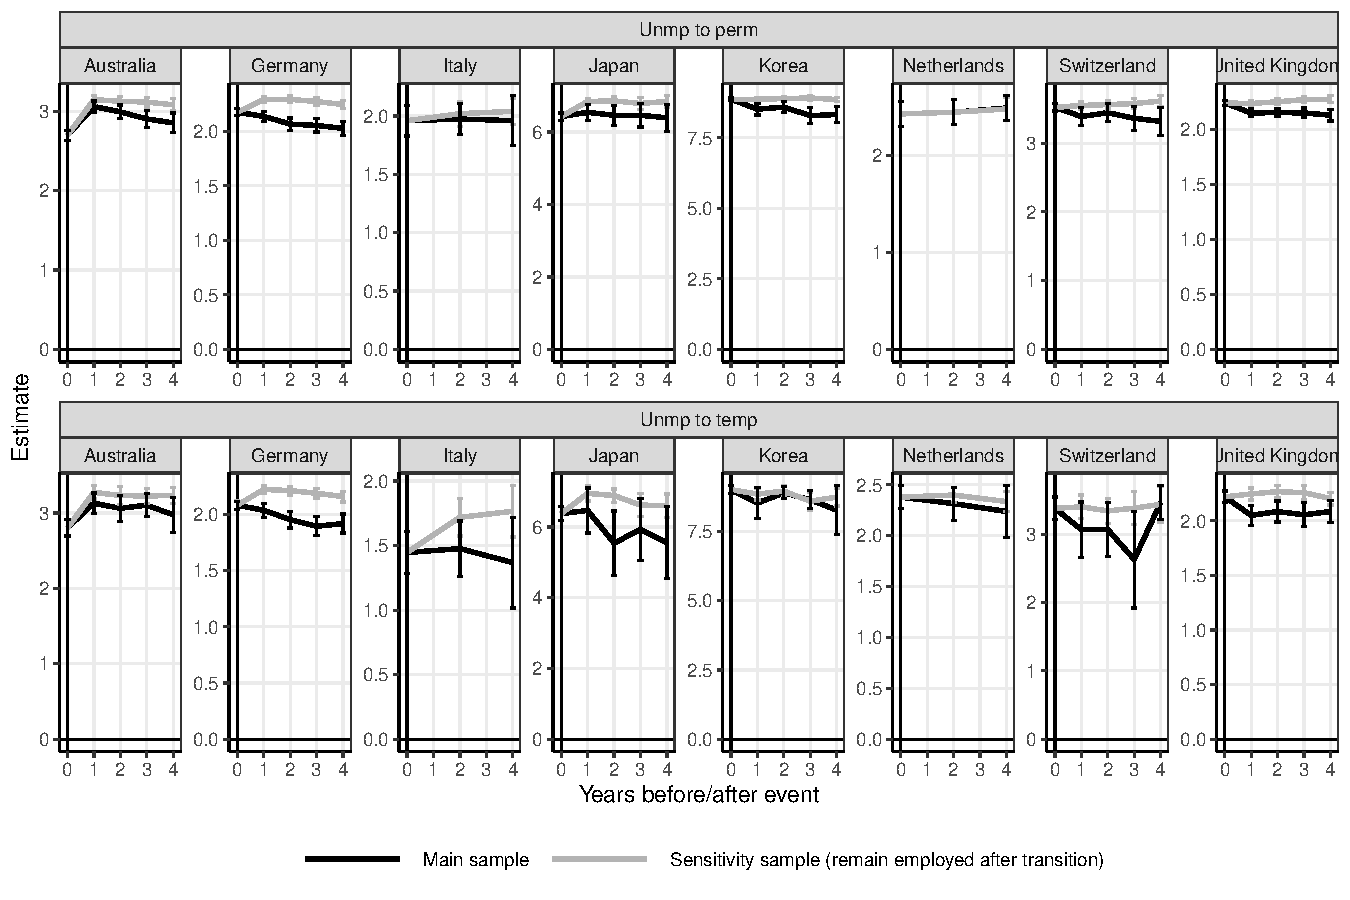
\includegraphics{../../../graphs/employed/graph_sensitivity_employed_post_2.pdf}}
    \label{graph_post_employed_2}
\end{sidewaysfigure}

\begin{sidewaysfigure}[!h]
    \caption{Graphical effect of transitions out of unemployment on wages over time with different samples (as compared to figure \ref{graph_unmp_post})}
    \resizebox{\textwidth}{!}{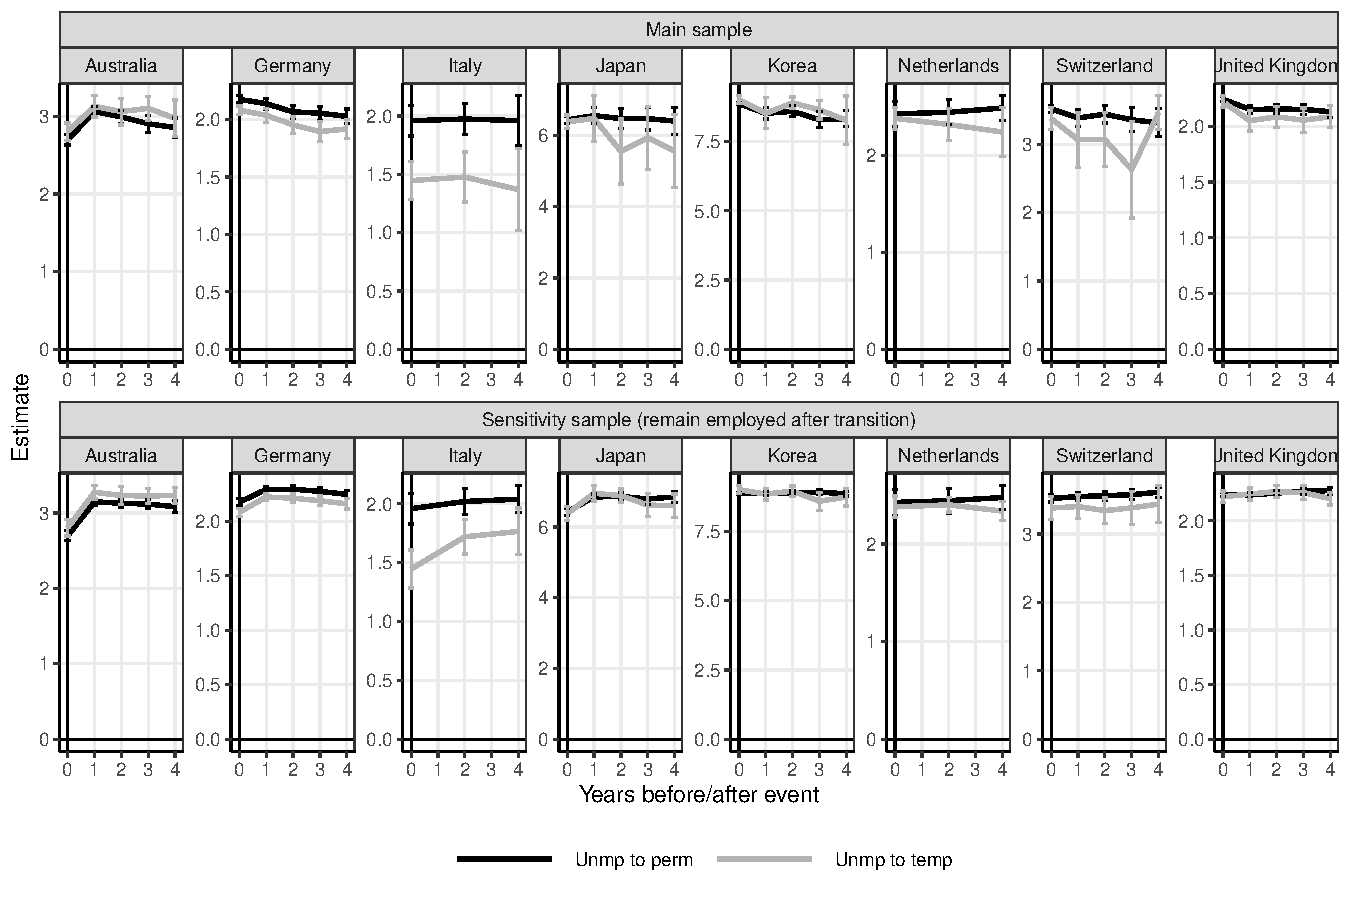
\includegraphics{../../../graphs/employed/graph_sensitivity_employed_post_1.pdf}}
    \label{graph_post_employed_1}
\end{sidewaysfigure}



%%%%%%%%%%%%%%%%%%%%%%%%%%%%%%%%%%%%%%%%%%
%%%%%%%%%%%%%%%%%%%%%%%%%%%%%%%%%%%%%%%%%%
%%%%%%%%%%%%%%%%%%%%%%%%%%%%%%%%%%%%%%%%%%
%%%%%%%%%%%%%%%%%%%%%%%%%%%%%%%%%%%%%%%%%%
\clearpage
\section{Appendix: Sensitivity to model specification}\label{appendix:sensitivity_model}
\setcounter{table}{0}
\setcounter{figure}{0}
\renewcommand*\thetable{\Alph{section}.\arabic{table}}
\renewcommand*\thefigure{\Alph{section}.\arabic{figure}}
\renewcommand{\theHfigure}{\Alph{section}.\arabic{table}}
\renewcommand{\theHtable}{\Alph{section}.\arabic{figure}}

In this section, we test the sensitivity of our model specification.  

First, we estimate both models \ref{eq:model_afe_temp} and \ref{eq:model_afe_unmp}.  We refer to these models as asymmetric fixed effect with dummy impact functions (AFE + DIF).  According to Rüttenauer and Ludwig \citeyearpar{ruttenauer_fixed_2020} the FE estimation may overestimate the treatment effect as it does not model confounding by heterogeneous trends, whereas FEIS may underestimate the treatment effect as it may not properly distinguish the treatment effect from heterogeneous trends. For these reasons, we ran sensitivity check by estimating models \ref{eq:model_afe_temp} and \ref{eq:model_afe_unmp} with FEIS + DIF.  These are shown in figures \ref{graph_compare_model_feis}.  Results are qualitatively similar.

Second, we compare results using a sample with multiple events (as in the main paper) to a sample with only the first event.  These are shown in figures \ref{graph_sensitivity_single_multiple_events}.  Results are qualitatively similar.

Third, we compare results in the main sample specification to a sensitivity sample where we drop or censor pre-treatment observations before the reference period and post-treatment variables greater than 4 periods after the event.  In annual data, pre-treatment observations are less than 1 period before the event and 2 periods before the event in biannual data.  Therefore, in the sensitivity sample, 0 refers only to for all observations that did not experience a given event.  In the main sample, 0 refers both to individuals who either did not experience a given event or experienced the event at least 3 periods before.  This is shown in figure \ref{graph_sensitivity_post_censoring}.  Results are qualitatively similar.

\begin{sidewaysfigure}
    \caption{Methods: FE + DIF (as in the paper) vs. FEIS + DIF}
    \resizebox{\textwidth}{!}{\includegraphics{../../../graphs/sensitivity/graph_compare_model_feis_paper.pdf}}
    \label{graph_compare_model_feis}
\end{sidewaysfigure}

\begin{sidewaysfigure}[!h]
    \caption{Compare multiple events (as in the paper) vs. first, single event}
    \resizebox{\textwidth}{!}{\includegraphics{../../../graphs/sensitivity/graph_sensitivity_single_multiple_events_paper.pdf}}
    \label{graph_sensitivity_single_multiple_events}
\end{sidewaysfigure}{}

% \begin{sidewaysfigure}[h!]
%     \caption{Effect of transitions between contract type on wages at point in time (as compared to figure \ref{graph_contyp})}
%     \resizebox{\textwidth}{!}{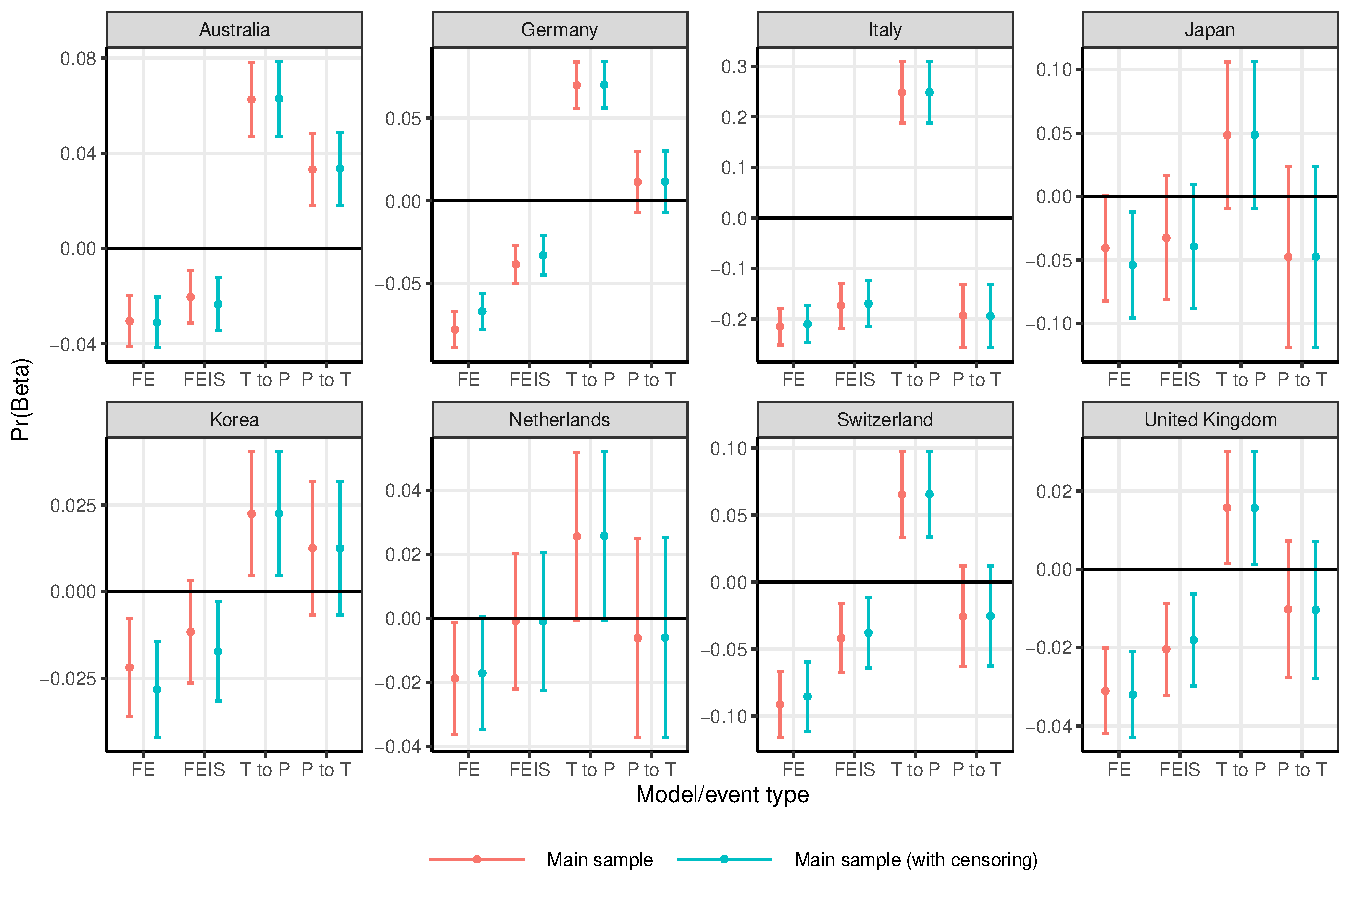
\includegraphics{../../../graphs/censoring/graph_sensitivity_compare_contyp_censoring.pdf}}
%     \label{graph_sensitivity_contyp_censoring}
% \end{sidewaysfigure}

% \begin{sidewaysfigure}
%     \caption{Effect of transitions out of unemployment by contract type on wages at point in time (as compared to figure \ref{graph_unmp})}
%     \resizebox{\textwidth}{!}{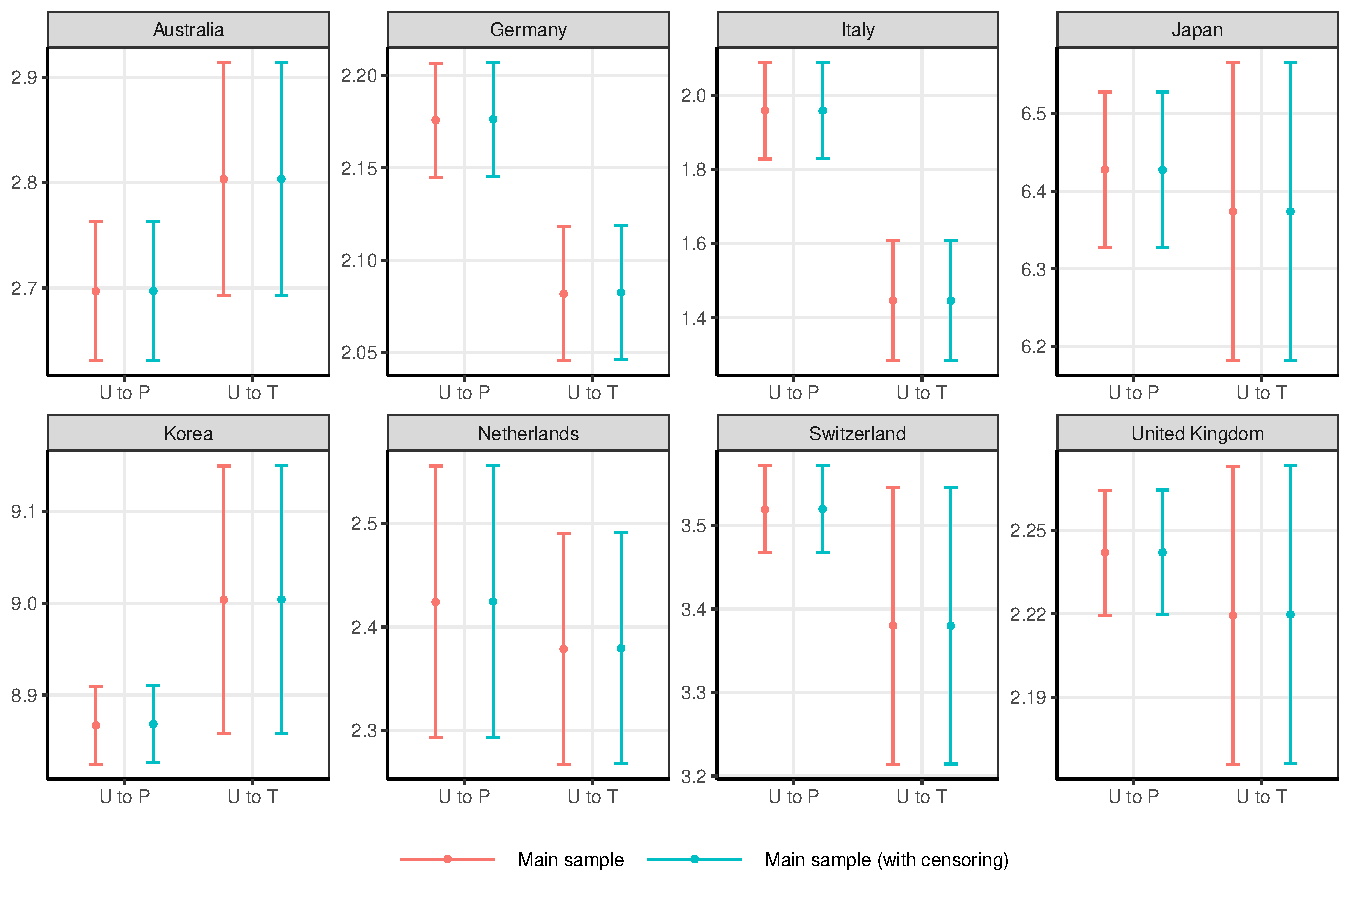
\includegraphics{../../../graphs/censoring/graph_sensitivity_compare_unmp_censoring.pdf}}
%     \label{graph_sensitivity_unmp_censoring}
% \end{sidewaysfigure}

\begin{sidewaysfigure}
    \caption{Graphical effect of transition on wages over time (as compared to figures \ref{graph_contyp_post} and  \ref{graph_unmp_post})}
    \resizebox{\textwidth}{!}{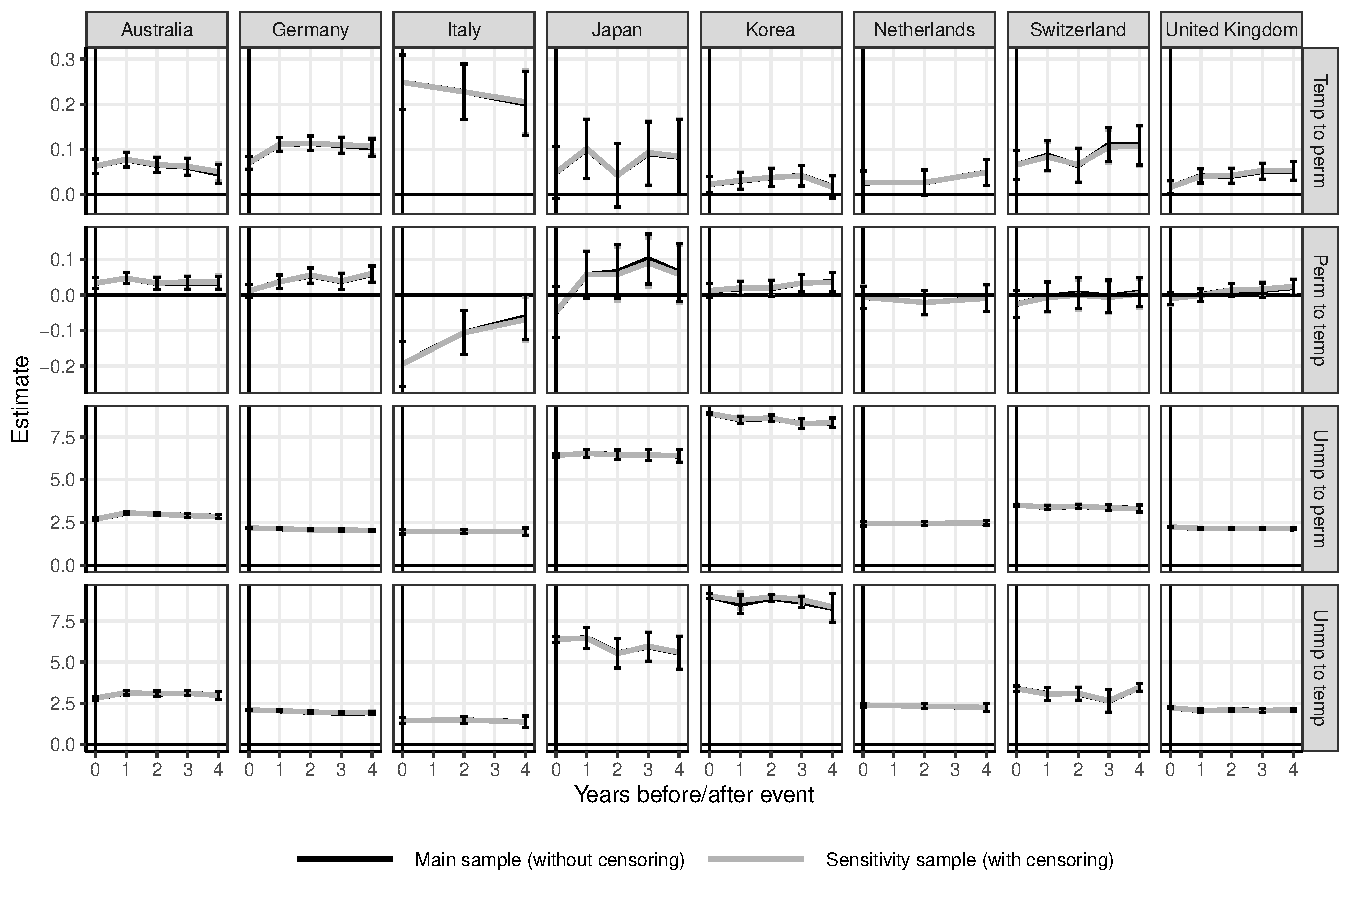
\includegraphics{../../../graphs/censoring/graph_sensitivity_censoring_post.pdf}}
    \label{graph_sensitivity_post_censoring}
\end{sidewaysfigure}


%%%%%%%%%%%%%%%%%%%%%%%%%%%%%%%%%%%%%%%%%%
%%%%%%%%%%%%%%%%%%%%%%%%%%%%%%%%%%%%%%%%%%
%%%%%%%%%%%%%%%%%%%%%%%%%%%%%%%%%%%%%%%%%%
%%%%%%%%%%%%%%%%%%%%%%%%%%%%%%%%%%%%%%%%%%
\clearpage
\section{Appendix: Results sensitivity}\label{appendix:sensitivity_variable}
\setcounter{table}{0}
\setcounter{figure}{0}
\renewcommand*\thetable{\Alph{section}.\arabic{table}}
\renewcommand*\thefigure{\Alph{section}.\arabic{figure}}
\renewcommand{\theHfigure}{\Alph{section}.\arabic{table}}
\renewcommand{\theHtable}{\Alph{section}.\arabic{figure}}

In this appendix, we examine the robustness of the results to distinct model specifications or definitions of event.  In Australia and in the United Kingdom, we compare different definitions of temporary employment (Figure \ref{graph_sensitivity_AU} and \ref{graph_sensitivity_AU}, respectively).  Further, in the Netherlands, we also compare results from the LSP to the LISS (Figure \ref{graph_sensitivity_NE}).  



\begin{sidewaysfigure}[!h]
    \caption{Australia: All temporary (incl. casual) vs. FTC only (as in the paper)}
    \resizebox{\textwidth}{!}{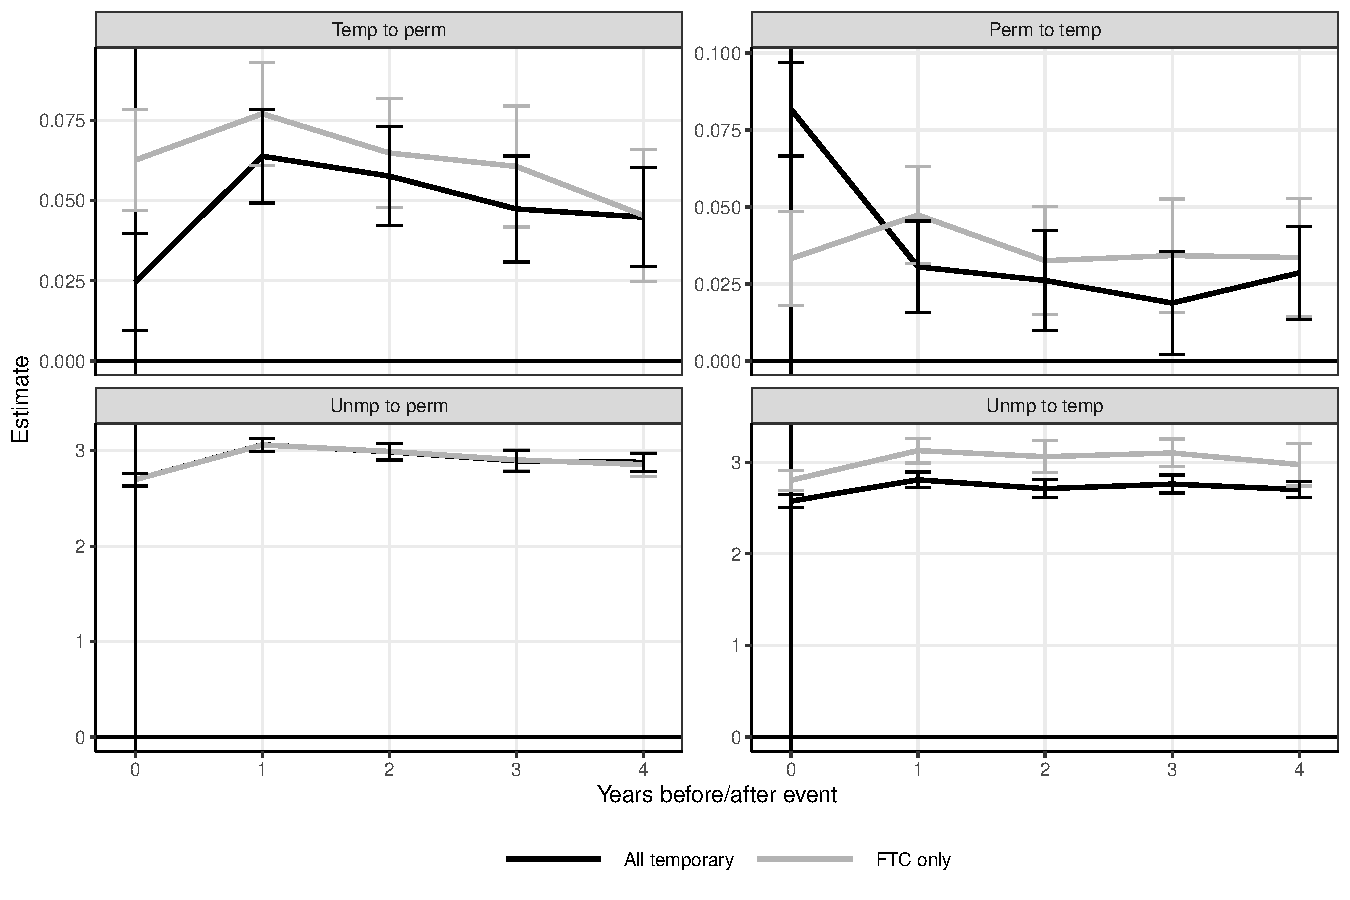
\includegraphics{../../../graphs/sensitivity/graph_sensitivity_AU_paper.pdf}}
    \label{graph_sensitivity_AU}
\end{sidewaysfigure}


\begin{sidewaysfigure}
    \caption{United Kingdom: All temporary (as in the paper) vs. FTC only}
    \resizebox{\textwidth}{!}{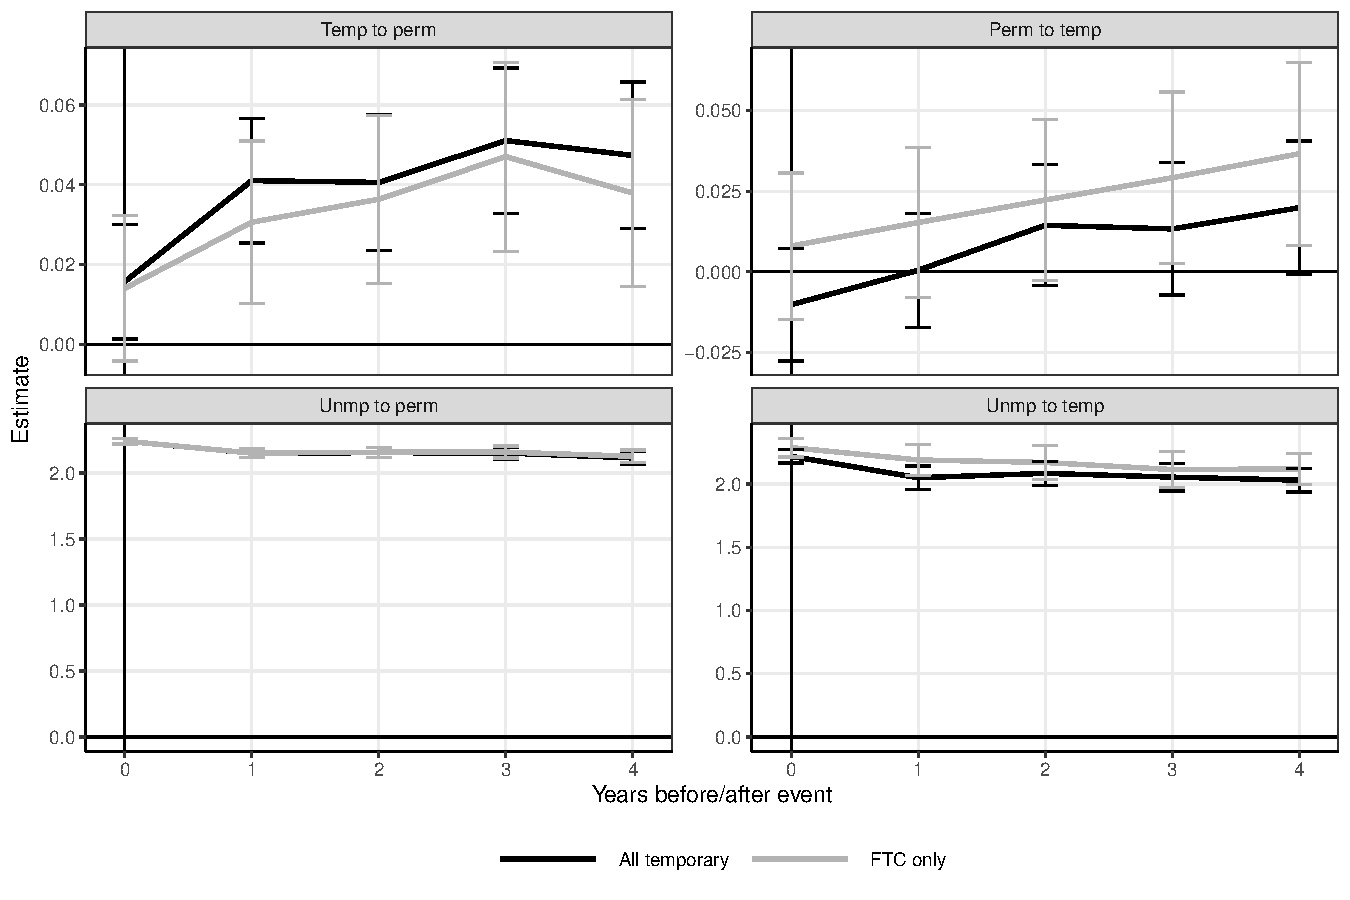
\includegraphics{../../../graphs/sensitivity/graph_sensitivity_UK_paper.pdf}}
    \label{graph_sensitivity_UK}
\end{sidewaysfigure}

\begin{sidewaysfigure}
    \caption{Netherlands: LSP (as in the paper) vs. LISS}
    \resizebox{\textwidth}{!}{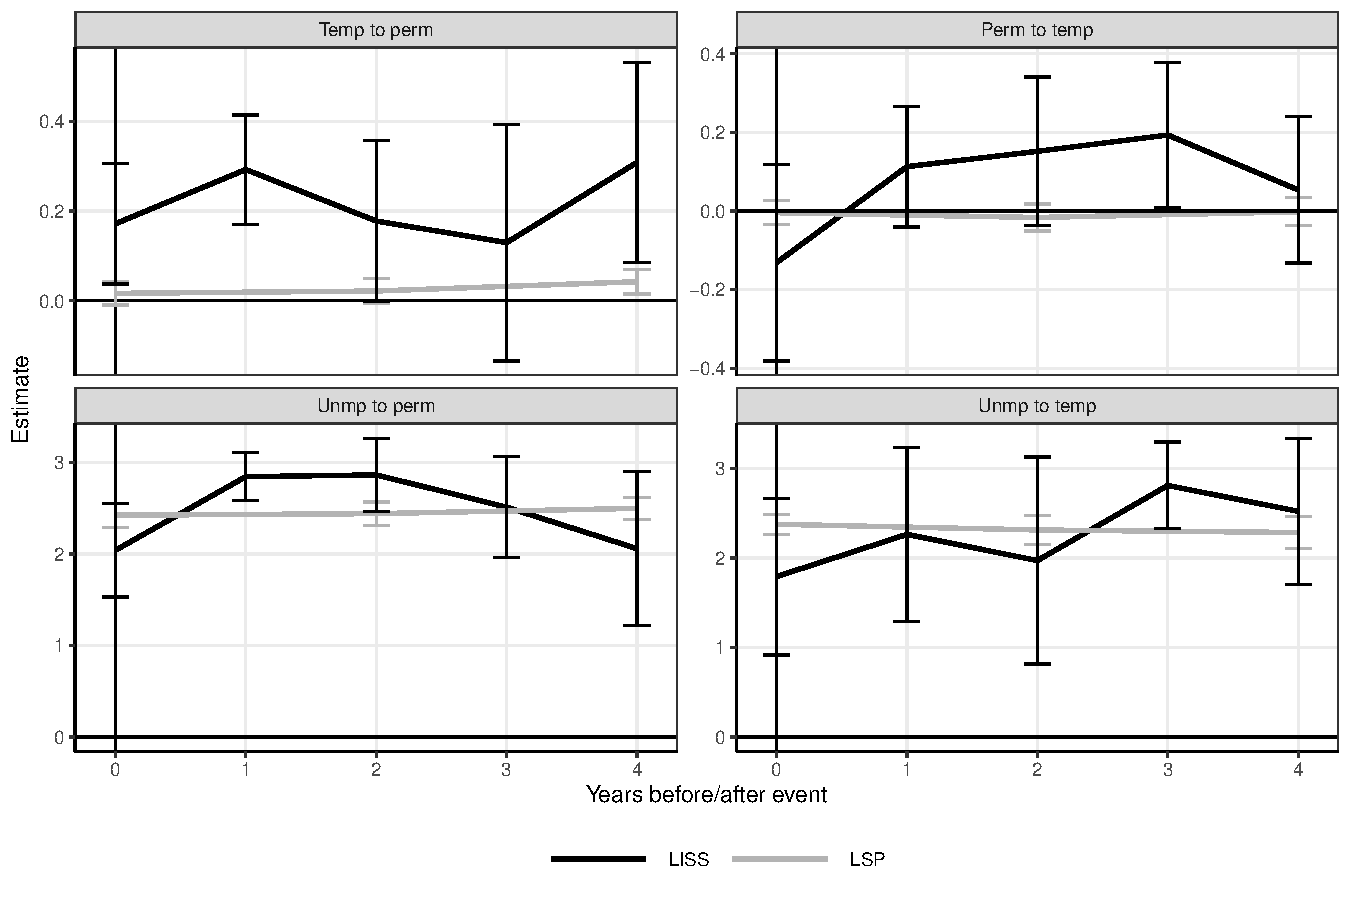
\includegraphics{../../../graphs/sensitivity/graph_sensitivity_NE_paper.pdf}}
    \label{graph_sensitivity_NE}
\end{sidewaysfigure}



%%%%%%%%%%%%%%%%%%%%%%%%%%%%%%%%%%%%%%%%%%
%%%%%%%%%%%%%%%%%%%%%%%%%%%%%%%%%%%%%%%%%%
%%%%%%%%%%%%%%%%%%%%%%%%%%%%%%%%%%%%%%%%%%
%%%%%%%%%%%%%%%%%%%%%%%%%%%%%%%%%%%%%%%%%%
\clearpage
\setcounter{table}{0}
\setcounter{figure}{0}
\renewcommand*\thetable{\Alph{section}.\arabic{table}}
\renewcommand*\thefigure{\Alph{section}.\arabic{figure}}
\renewcommand{\theHfigure}{\Alph{section}.\arabic{table}}
\renewcommand{\theHtable}{\Alph{section}.\arabic{figure}}

\section{Appendix: Results heterogeneity}\label{appendix:sensitivity_heterogeneity}

We conducted a series of robustness checks, which we broadly split into two categories.  In appendix \ref{appendix:sensitivity_variable}, we examine the robustness of the results to distinct model specifications or definitions of event.  In this appendix, we examine the robustness of the results to distinct heterogeneous groups, as shown in Appendix \ref{appendix:sensitivity_heterogeneity}.  Figure \ref{graph_post_event_age_cat} compares age groups (25-34, 35-44, and 45-54), figure \ref{graph_post_event_edu_cat} compares education groups (less than secondary, secondary, and more than secondary education), and figure \ref{graph_post_event_gender} compares results for men and women.  All results are qualitatively similar.

\begin{sidewaysfigure}[!h]
    \caption{Figures \ref{graph_contyp_post} and \ref{graph_unmp_post}, by age category}
    \resizebox{\textwidth}{!}{\includegraphics{../../../graphs/heterogeneity/graph_post_event_age_cat.pdf}}
    \label{graph_post_event_age_cat}
\end{sidewaysfigure}

\begin{sidewaysfigure}[!h]
    \caption{Figures \ref{graph_contyp_post} and \ref{graph_unmp_post}, by education category}
    \resizebox{\textwidth}{!}{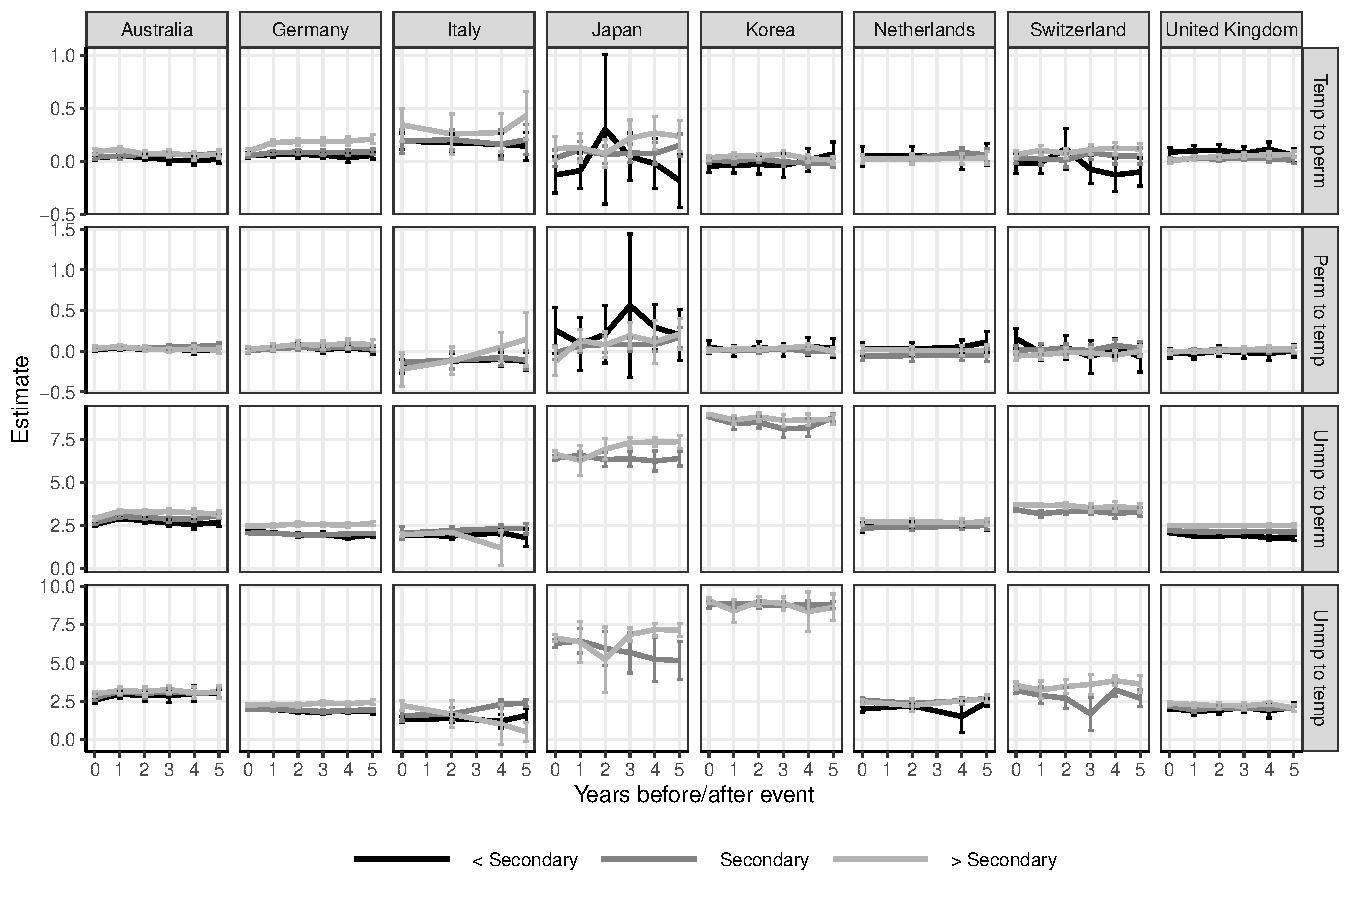
\includegraphics{../../../graphs/heterogeneity/graph_post_event_edu_cat.pdf}}
    \label{graph_post_event_edu_cat}
\end{sidewaysfigure}

\begin{sidewaysfigure}[!h]
    \caption{Figures \ref{graph_contyp_post} and \ref{graph_unmp_post}, by gender}
    \resizebox{\textwidth}{!}{\includegraphics{../../../graphs/heterogeneity/graph_post_event_gender.pdf}}
    \label{graph_post_event_gender}
\end{sidewaysfigure}




%%%%%%%%%%%%%%%%%%%%%%%%%%%%%%%%%%%%%%%%%%
%%%%%%%%%%%%%%%%%%%%%%%%%%%%%%%%%%%%%%%%%%
%%%%%%%%%%%%%%%%%%%%%%%%%%%%%%%%%%%%%%%%%%
%%%%%%%%%%%%%%%%%%%%%%%%%%%%%%%%%%%%%%%%%%
\end{document}

